%%%%%%%%%%%%%%%%%%%%%%%%%%%%%%%%%%%%%%%%%%%%%%%%%%%%%%%%%%%%%%%%%%%%%%%%%%%%%
%%%
%%% File: thesis.tex, version 1.9, May 2016
%%%
%%% =============================================
%%% This file contains a template that can be used with the package
%%% cs.sty and LaTeX2e to produce a thesis that meets the requirements
%%% of the Computer Science Department from the Technical University of Cluj-Napoca
%%%%%%%%%%%%%%%%%%%%%%%%%%%%%%%%%%%%%%%%%%%%%%%%%%%%%%%%%%%%%%%%%%%%%%%%%%%%%

\documentclass[12pt,a4paper,twoside]{report}         
\usepackage{cs}
\usepackage{subfig}
\usepackage{wrapfig}
\usepackage{svg}
\usepackage{float}
\usepackage{fancyvrb}
\usepackage{listings}
\usepackage{rotating}
\usepackage{amsmath}
\usepackage{times}
\usepackage{graphicx}
\usepackage{latexsym}
\usepackage{amsmath,amsbsy}
\usepackage{amssymb}
\usepackage[matrix,arrow]{xy}
\usepackage[T1]{fontenc}
\usepackage{ae,aecompl}
\usepackage{romanian} %definitii pentru diacritice; 
\usepackage{amstext}
\usepackage{graphics}
\usepackage[T1]{fontenc}
\usepackage{ae,aecompl}
% \usepackage{algorithm}
%\usepackage{algorithmic}
% \usepackage{color}
\usepackage{color}
\usepackage{algorithm}
\usepackage{algorithmic}
% \mastersthesis
\diplomathesis
% \leftchapter
\centerchapter
% \rightchapter
\singlespace
% \oneandhalfspace
% \doublespace

\renewcommand{\thesisauthor}{Andrei MORARU}    %% Your name.
\renewcommand{\thesismonth}{Iulie}     %% Your month of graduation.
\renewcommand{\thesisyear}{2022}      %% Your year of graduation.
\renewcommand{\thesistitle}{URM'ARIREA UNUI OBIECT PRIN FUZIUNE SENZORIAL'A} % Title
\renewcommand{\thesissupervisor}{Prof. dr. ing. Eva H. DULF}
\newcommand{\department}{FACULTATEA DE AUTOMATIC'A 'SI CALCULATOARE\\
DEPARTAMENTUL AUTOMATIC'A}
\newcommand{\thesis}{LUCRARE DE LICEN'T'A}
\newcommand{\uline}[1]{\rule[0pt]{#1}{0.4pt}}
%\renewcommand{\thesisdedication}{P'arin'tilor mei}
\newcommand{\utcnlogo}{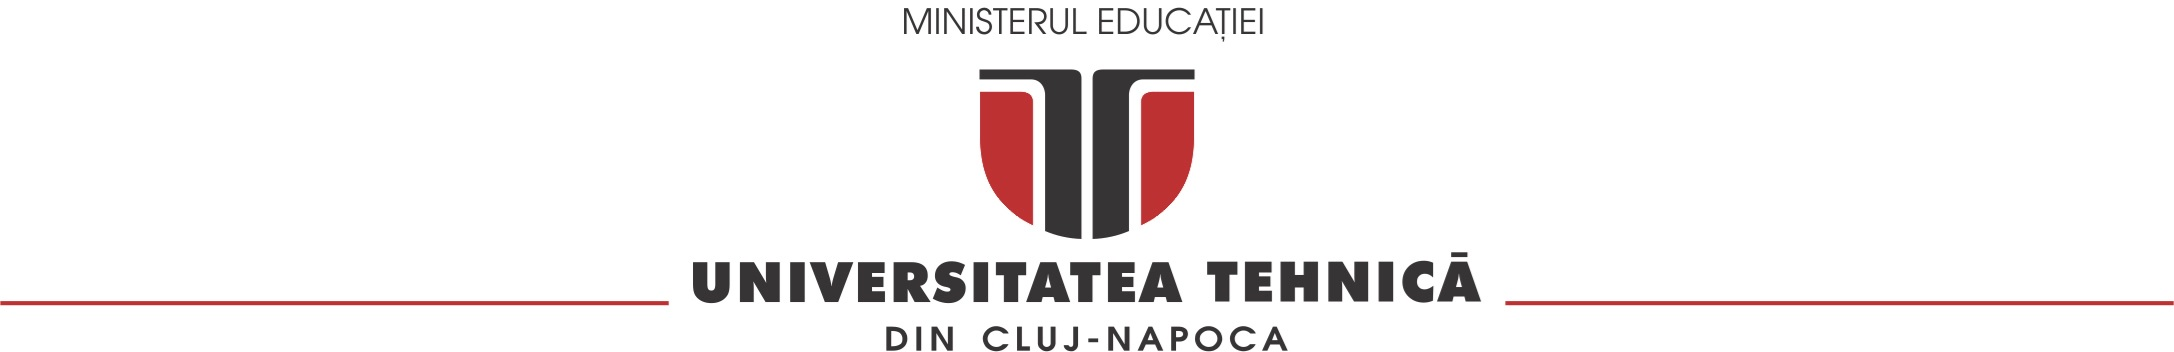
\includegraphics[width=15cm]{img/utcn.jpg}}

\begin{document}
%\frontmatter
%\pagestyle{headings}

\newenvironment{definition}[1][Defini'tie.]{\begin{trivlist}
\item[\hskip \labelsep {\bfseries #1}]}{\end{trivlist}}



%\thesistitle                    %% Generate the title page.
%\authordeclarationpage                %% Generate the declaration page.


\begin{center}
%\includegraphics[width=15cm]{img/tucn.jpg}  
\utcnlogo

{\bf \department}

\vspace{4cm}

{\bf \thesistitle} %LICENSE THESIS TITLE}

\vspace{1.5cm}

\thesis

\vspace{6cm}

Absolvent: {\bf \thesisauthor} 

Conduc'ator 'stiin'tific: {\bf \thesissupervisor}

\vspace{3cm}
{\bf \thesisyear}
\end{center}

\thispagestyle{empty}
\newpage

\begin{center}
\utcnlogo

{\bf \department}
\end{center}
\vspace{0.5cm}

%\begin{small}
\begin{tabular}{p{7cm}p{8cm}}
 %\hspace{-1cm}& VIZAT,\\
 \hspace{-1cm}DECAN, & DIRECTOR DEPARTAMENT,\\
\hspace{-1cm}{\bf Prof. dr. ing. Liviu MICLEA} & {\bf Prof. dr. ing. Honoriu V'ALEAN}\\  
\end{tabular}
 
\vspace{2cm}

\begin{center}
Absolvent: {\bf \thesisauthor}

\vspace{1cm}

{\bf \thesistitle}
\end{center}

\vspace{1cm}

\begin{enumerate}
 \item {\bf Enun'tul temei:} {\it Diverse metode de estimare a traiectoriei prin fuziune senzorial'a 'in vederea realiz'arii unei urm'ariri autonome a unui obicect 'in planul bidimensional}
\item {\bf Con'tinutul lucr'arii:} {\it Cuv\ia nt-'inainte, Obiective, Studiu Bibliografic, Analiz'a 'si Fundamentare Teoretic'a, Proiectare de Detaliu 'si Implementare, Testare 'si Validare, Manual de Instalare 'si Utilizare, Concluzii, Anexele A,B,C}
\item {\bf Locul document'arii:} {\it Universitatea Tehnic'a din Cluj-Napoca, Departamentul Automatic'a}
\item {\bf Consultan'ti: Prof. dr. ing. Zsófia LENDEK}
\item {\bf Data emiterii temei:} 1 Octombrie 2021
\item {\bf Data pred'arii:} 1 iulie 2022 
 \end{enumerate}
\vspace{1.2cm}

\hspace{5cm} Absolvent: \uline{3cm}

\vspace{0.5cm}
\hspace{5cm} Coordonator 'stiin'tific: \uline{3cm}
%\end{small}

\thispagestyle{empty}

\newpage

\begin{center}
\utcnlogo

{\bf \department}
\end{center}

\vspace{0.5cm}

\begin{center}
{\bf
Declara'tie pe proprie r'aspundere privind\\ 
autenticitatea lucr'arii de licen't'a}
\end{center}
\vspace{1cm}



Subsemnatul \textit{Moraru Andrei}, 
legitimat cu \textit{cartea de identitate} seria \textit{MH} nr. \textit{550346}
CNP \textit{1990920055053}, autorul lucr'arii \textit{URM'ARIREA UNUI OBIECT PRIN FUZIUNE SENZORIAL'A}
elaborat'a 'in vederea sus'tinerii examenului de finalizare a studiilor de licen't'a la Facultatea de Automatic'a 'si Calculatoare, Specializarea \textit{Ingineria Sistemelor Automate} din cadrul Universit'a'tii Tehnice din Cluj-Napoca, sesiunea \textit{iulie} a anului universitar \textit{2022}, declar pe proprie r'aspundere, c'a aceast'a lucrare este rezultatul propriei activit'a'ti intelectuale, pe baza cercet'arilor mele 'si pe baza informa'tiilor ob'tinute din surse care au fost citate, 'in textul lucr'arii 'si 'in bibliografie.

Declar, c'a aceast'a lucrare nu con'tine por'tiuni plagiate, iar sursele bibliografice au fost folosite cu respectarea legisla'tiei rom\ia ne 'si a conven'tiilor interna'tionale privind drepturile de autor.

Declar, de asemenea, c'a aceast'a lucrare nu a mai fost prezentat'a 'in fa'ta unei alte comisii de examen de licen't'a.

'In cazul constat'arii ulterioare a unor declara'tii false, voi suporta sanc'tiunile administrative, respectiv, \emph{anularea examenului de licen't'a}.

\vspace{1.5cm}

Data \hspace{8cm} Nume, Prenume

\vspace{0.5cm}

\textit{01.07.2022} \hspace{6.9cm} \textit{Moraru Andrei}

\vspace{1cm}
\hspace{9.4cm}Semn'atura

\thispagestyle{empty}


\newpage

\begin{center}
\utcnlogo

{\bf \department}
\end{center}

\vspace{0.5cm}

\begin{center}
{\bf
SINTEZA \\
proiectului cu titlul:} \\
{\bf \thesistitle}
\end{center}
\vspace{1cm}

\begin{enumerate}
 \item {\bf Cerin'tele temei:} {\it Proiectarea unei aplica'tii care s'a simuleze o curs'a interactiv'a cu scopul de a pune 'in practic'a diver'si algoritmi de estimare, reprezent'ari ale orient'arii 'in spa'tiu 'si legi de control}
\item {\bf Solu'tii alese:} {\it Filtre Kalman - liniar, extins 'si unscented, cuaternioni, control liniar}
\item {\bf Rezultate ob'tinute:} {\it Convengen'ta garantat'a pentru sisteme liniare, solu'tii func'tionale pentru modele neliniare, 'imbun'at'a'tirea timpului de r'aspuns comparativ cu implement'ari alternative}
\item {\bf Test'ari 'si verific'ari}: {\it Compara'tia cu solu'tii deja existente, valid'ari grafice, valid'ari numerice prin minimizarea erorilor}
\item {\bf Contribu'tii personale:}  {\it Implementarea unei aplica'tii complexe bazat'a pe programare orientat'a pe obiecte ce se prezint'a ca o abordare diferit'a a fundamentului teoretic, realizarea unei solu'tii alternative de estimare a orient'arii pentru o fun'ctionalitate deja existent'a, dezvoltarea interac'tiunilor 'si anima'tiilor din joc, conceperea interfe'tei grafice, realizarea conexiunii cu o plac'a de dezvoltare Arduino Nano 'intr-o configura'tie personal'a de tip joystick}
\item {\bf Surse de documentare}: {\it Publica'tii 'stiin'tifice, articole 'si site-uri de specialitate, surse video, consulta'tii 'in timpul 'si 'in afara orelor de curs cu profesorii} 
 \end{enumerate}
\vspace{1.2cm}

\thispagestyle{empty}

\newpage

%\clearpage 
%\newpage

%\begin{comment}
% {\color{red}{\bf De citit 'inainte} (aceast'a pagin'a se va elimina din versiunea final'a)}:
\begin{enumerate}
 \item Cele trei pagini anterioare (foaie de cap'at, foaie sumar, declara'tie) se vor lista pe foi separate (nu fa't'a-verso), fiind incluse 'in lucrarea listat'a. 
 Foaia de sumar (a doua) necesit'a semn'atura absolventului, respectiv a coordonatorului.
 Pe declara'tie se trece data c\ia nd se pred'a lucrarea la secretarii de comisie.
 \item Pe foaia de cap'at, se va trece corect titulatura cadrului didactic 'indrum'ator, 'in englez'a (consulta'ti pagina de unde a'ti desc'arcat acest document pentru lista cadrelor didactice cu titulaturile lor).
 \item Documentul curent {\bf nu} a fost creat 'in MS Office. E posibil sa fie mici diferen'te de formatare. 
\item Cuprinsul 'incepe pe pagina nou'a, impar'a (dac'a se face listare fa't'a-verso), prima pagin'a din capitolul Introducere tot a'sa, fiind numerotat'a cu 1. % Pentru actualizarea cuprinsului, click dreapta pe cuprins (zona cuprinsului va apare cu gri), Update field-$>$Update entire table.
\item Vizualiza'ti (recomandabil 'si 'in timpul edit'arii) acest document % după ce activaţi vizualizarea simbolurilor ascunse de formatare (apăsaţi simbolul  din Home/Paragraph).
\item Fiecare capitol 'incepe pe pagin'a nou'a. % datorită simbolului ascuns Section Break (Next Page) care este deja introdus la capitolul precedent. Dacă ştergeţi din greşeală simbolul, se reintroduce (Page Layout -> Breaks).
\item Folosi'ti stilurile predefinite (Headings, Figure, Table, Normal, etc.)
\item Marginile la pagini nu se modific'a.
\item Respecta'ti restul instruc'tiunilor din fiecare capitol.
\end{enumerate}
\thispagestyle{empty} 
%\end{comment}

\pagenumbering{roman}
\setcounter{page}{1}

\newpage

\tableofcontents

\newpage

%\listoftables
%\listoffigures

\pagenumbering{arabic}
\setcounter{page}{1}

\chapter{Cuv\ia nt-'inainte}

\section{Despre 'stiin't'a 'si zgomot}

\textit{"Atunci c\ia nd nu 'stii ce faci, toate calculele tale sunt zgomot"} este dictonul propriu enun'tat de Rudolf Emil Kalman 'intr-un colocviu sus'tinut la Institutul de tehnologie din Massachusetts 'in 1991 \footnote{https://www.youtube.com/watch?v=i5kTdHT3yBg}, ca o concluzie personal'a cu privire la aleatoritatea reg'asit'a 'in fenomenele lumii reale. 

\vspace{5px}

Privit'a 'in contextul teoriei sistemelor, maxima 'isi redob\ia nde'ste terenul cedat 'in favoarea senten'tiozit'a'tii, pentru c'a spusele autorului 'i'si reg'asesc efectul 'in lucr'ari istorice care se bucur'a 'si ast'azi de o general'a aplicabilitate, lucr'ari care stau 'si la baza prezentei teze de diplom'a. 

\vspace{5px}

De'si nu singurul canevas de suport teoretic pentru actuala lucrare, stocasticitatea sistemelor reale este cu siguran't'a una din lentilele prin care poate fi analizat acest studiu, dar 'in acela'si timp 'si un instrument utlil pentru a trage concluzii pertinente cu privire la rezultatele ob'tinute; 'si tocmai de aceea am ales s'a 'ii ofer 'insemn'atatea cuvenit'a 'in contextul problematicei fuziunii senzoriale pentru sistemele neliniare.

\vspace{5px}

Doresc, pe aceast'a cale, s'a introduc subiectul lucr'arii mele de licen't'a printr-o sintez'a a contextului actual ce a iscat interesul personal pentru algoritmii reg'asi'ti pe ramura statistic-probabilistic'a a teorei sistemelor, teorie ce reprezint'a fundamentul modelelor matematice din spatele func'tion'arii senzorilor iner'tiali.   

\vspace{5px}

Am ales s'a dezvolt acest proiect 'in jurul unei aplica'tii de urm'arire 'in timp real a unui obiect, deoarece consider c'a acesta este unul dintre scenarile prin care se poate observa cel mai clar necesitatea 'imbin'arii tututror resurselor senzoriale posibile 'in vederea ob'tinerii unui peisaj c\ia t mai clar despre cadrul imediat 'inconjur'ator 'in care se desf'a'soar'a mi'scarea. Din acest motiv am decis s'a proiectez 'si o aplica'tie interactiv'a prin intermediul c'areia punerea 'in practic'a a no'tiunilor teoretice se realizeaz'a print-un cadru aparent ingenuu, dar cu implicare direct'a 'si consolidat de o analiz'a minu'tioas'a 'in spate.


\section{Senzorii iner'tiali}

Motivul central al acestei lucr'ari este, f'ar'a 'indoial'a, dup'a cum este evocat 'si 'in titlu, reprezentat de senzori, 'in deosebi de cei iner'tiali. Ace'stia pot fi privi'ti cu interes din mai multe puncte de vedere, 'in special pentru importan'ta din prezent acordat'a 'inglob'arii lor 'in c\ia t mai multe dispozitive, dar 'si pentru evolu'tia lor electronic'a din ultimele decenii. 'In lucrarea propus'a 'ins'a, abordarea pe care doresc s'a o aprofundez se refer'a la modelele matematice din spatele informa'tiei ob'tinute de la senzori, mai mult dec\ia t la senzori 'in sine, de'si avantajele 'si limit'arile lor vor fi de asemenea amintite. 

\vspace{5px}

Senzorii iner'tiali sunt o parte vital'a a procesului de realizare a sistemelor autonome 'si fac parte din ciclul de proceduri SPPA (Sense, Percieve, Plan, Act) ' in procesele de control ce adreseaz'a sectorul roboticii sau al vehiculelor inteligente. Tocmai de aceea am decis s'a conturez contextul acestui proiect ca unul specific industriei automobilistice, particularizat pentru procedurile de fuziune senzorial'a. Dedic astfel urm'atoarele capitole unei analize riguroase a prezentelor tehnici 'si metodologii folosite actual 'in domeniu 'si ofer 'si o implementare bazat'a pe cunos'tiin'tele acumulate menite s'a serveasc'a ca schelet pentru ulterioarele proiecte ce vor urma.


\section{Aprecieri}

Prezenta lucrare nu ar fi fost complet'a f'ar'a 'indumarea oferit'a de prof. dr. ing Eva Henrieta Dulf, conduc'atoarea 'stiin'tific'a a tezei mele de diplom'a 'si de aceea doresc 'in acest capitol introductiv s'a ii mul'tumesc pentru 'indemnurile oferite 'si constantele 'incuraj'ari.

\vspace{5px}

Tot 'intr-at\ia t de recunosc'ator ii sunt 'si doamnei profesoare dr.ing. Zsófia Lendek pentru ajutorul constant 'si implicarea direct'a acordate 'in timpul ultimul semestru pentru implementarea algoritmilor de estimare folosi'ti 'in aplica'tia final'a, cel mai avansat reg'asindu-se 'intr-una din anexele acestui document.  

\vspace{5px}

Sunt recunosc'ator de asemenea 'si pentru 'indrumarea oferit'a de MSc. ing. Daniel D. Timi's 'in cadrul unui proiect care a devenit stadiul incipient al acestei lucr'ari de licen't'a 'in urm'a cu un an universitar. 

% Lumea senzorilor

\pagestyle{headings}

% Titlul capitolului se bazeaz'a pe Heading 1 style, numerotat cu o cifra (x. Nume capitol), font Times New Roman de 14, Bold.

% Ce se scrie aici:

% \begin{itemize}
%  \item Contextul
% \item Conturarea domeniului exact al temei
% \item Reprezint'a cca. 5\% din lucrare
% \end{itemize}


% Fontul folosit implicit 'in acest document este Times New Roman, dimensiune de 12, conform Normal style, cu spa'tiere la 1 r\ia nd (Paragraph, Line spacing de 1.0) 'si Justify. 
% Pentru prima linie din fiecare paragraf se folose'ste indentare (implicit 'in Normal Style), iar 'intre paragrafe succesive nu se las'a distan't'a suplimentar'a\footnote{Sunt rezolvate automat de Latex}.

% \subsection{Subsection}
% Fiecare tabel introdus 'in lucrare este numerotat astfel: Tabel x.y, unde x reprezint'a num'arul capitolului iar y num'arul tabelului din capitol. 
% Se las'a un r\ia nd liber 'intre tabel 'si paragraful anterior, respectiv posterior (table~\ref{table:nonlin}).

% \begin{table}[ht]
% \caption{Rezultate}
% \centering                          % tabel centrat 
% \begin{tabular}{|c|c|c|c|}          % 4 coloane centrate 
% \hline\hline                        % linie orizontala dubla
% Case & Method\#1 & Method\#2 & Method\#3 \\ [0.5ex]   % inserare tabel
% %heading
% \hline                              % linie orizontal simpla
% 1 & 50 & 837 & 970 \\               % corpul tabelului 
% 2 & 47 & 877 & 230 \\
% 3 & 31 & 25 & 415 \\[1ex]           % [1ex] adds vertical space
% \hline                              
% \end{tabular}
%   % titlul tabelului
% \label{table:nonlin}                % \label{table:nonlin} introduce eticheta folosita pentru referirea tabelului in text; referirea in text se va face cu \ref{table:nonlin}
% \end{table}

% Fiecare figur'a introdus'a 'in text este citat'a (de ex: 'in figura x.y este prezentat'a ...) 'si numerotat'a. 
% Numerotarea se face astfel Figura x.y unde x reprezint'a num'arul capitolului iar y num'arul figurii 'in acel capitol. 
% E.g.: figure~\ref{fig:imag}.

% \begin{figure}[ht]
%     \centering
% 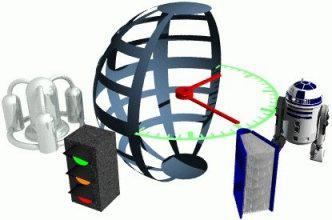
\includegraphics[]{img/test.jpg}
%     \caption{Numele figurii}
%     \label{fig:imag}
% \end{figure}

% Fiecare capitol 'incepe pe pagin'a nou'a.

\chapter{Obiectivele Proiectului}

% 'In acest capitol se prezint'a tema propriu-zis'a (sub forma unei teme de proiectare sau cercetare, formulat'a exact, cu obiective clare - 2-3 pagini 'si eventuale figuri explicative).

% Reprezint'a cca. 10\% din lucrare.
% \section{Titlu}
% \section{Alt titlu}

Definit'a ca schimbarea poziției în raport cu timpul, mișcarea poate fi modelat'a cu un set de dou'a ecua'tii diferen'tiale. Indiferent de tipul și complexitatea traiectoriei pe care o definește corpul în mișcare, și fară a 'tine seama de masa ori de volumul corpului imaginat, locul geometric definit de proiecția poziției obiectului animat pe axele unui plan sau ale unui spatiu se supune dinamicii definit'a întotdeauna de acelea'si dou'a ecuații specifice. Aceste legi bine definite inițial de Galileo Galilei, și concretizate mai apoi de Isaac Newton, fac posibila descrierea mișcării în univers în general, și a corpurilor de pe pământ în particular. Comportamentul ce se împotrivește inerției poate fi, cu ajutorul soluțiilor ecuațiilor diferențiale, modelat ca un sistem dinamic al c'arei component'a cinematic'a este dat'a întocmai de acțiunea mișcării. Un astfel de sistem poate fi mai departe supus algoritmilor de estimare și legilor de control formulate de teoria sistemelor 'in func'tie de problematica domeniului pentru care este modelat. 

Am dezvoltat acest proiect cu scopul de a testa și valida diferiți algoritmi de estimare a traiectoriei unui obiect urmărit și legi de control care definesc acțiunile unui obiect urmăritor. O atenție deosebit'a a fost acordat'a metodelor de fuziune a măsurătorilor senzorilor și de exprimare a mișcărilor rotative în spa'tiul tridimensional. În acest sens, simularea urmăririi unei traiectorii este supleat'a de conectarea unui microcontroller Arduino care, prin intermediul unui modul extern de senzori inerțiali, permite utilizatorului să simuleze mișcarea obiectului urmărit, întocmai ca într-un joc ce se desfășoară în planul bidimensional al monitorului. 

Proiectul se împarte așadar în dou'a parti principale cu importan't'a de sine stătătoare, urmărirea traiectoriei simulate pentru obiectul în mișcare și fuziunea datelor de la senzor pentru generarea mișcării. Atât algoritmii de urmărire, cât și cei de fuziune, cu impact individual demn de menționat, sunt înrudiți prin teoria ce st'a la baza lor, și  formează împreună, în esență, o reprezentație mai fidela a realității care poate fi explorat'a mai departe în domenii precum conducerea autonom'a, realitatea virtual'a ori augmentat'a, precum și viitoarele lor posibile ramificații.

\section{Estimarea traiectoriei}


Pentru a realiza detecția poziției unui corp și pentru a iniția urmărirea acestuia, toți algoritmii folosiți până în prezent au că fundament în alcătuiră lor statistica descriptiv'a. Fenomenul mișcării, precum și cel al detecției acesteia prin folosirea senzorilor inerțiali, sunt măsurabile în timp pentru un grup de eșantioane de date, ceea ce face posibile concluzile legate de tendința centrala 'si dispersia grupului de m'asur'atori folosite, ce duc mai departe la rezultate validate prin acuratețe sau precizie, concepte ce pot fi concret definite prin termeni statistici. Pentru a studia dac'a modelul propus menit s'a descrie fenomenul este unul general, ce se dovede'ste fezabil și pentru aplicații de dimensiuni mai mari, statistica inferential'a este de aceast'a dat'a ramura relevant'a a științei probabilistice.

\vspace{5px}

Procedeele care se bazează pe noțiuni statistice au evoluat până în prezent pentru a fi folosite în combinație cu o mare gam'a de științe precum teoria controlului, informatica aplicat'a, dar și bilogia, psihologia ori științele umane, cu scopul de a găsi răspunsuri la întrebările din spatele unor fenomene naturale. Statistica aplicat'a culminează cu apariția metodelor de învățare automata, numita și inteligenta artificial'a, un obiect de studiu cu orizonturi nenumărate. 

\vspace{5px}

Algoritmii clasici de estimare, elocvenți teoriei sistemelor, au, fa't'a de relativ noile metode de învățare automata, avantajul că funcționarea lor este garantata din prima executare, fară a necesita o perioad'a de timp de antrenare, și fară a face greșeli, cu condiția ferm'a de a avea un model al procesului bine definit pentru sistemul dinamic aferent. Parametrii sistemului configurați pot fi estimați în timpul rulării, ceea ce face aceste proceduri fiabile întocmai pentru aplicații de timp real. Ca urmare, desi robuști prin informația codificat'a în implementarea lor, dezavantajul lor este că o convergen't'a general'a nu poate fi asigurat'a pentru orice scenariu. După cum se va observa în capitolul \ref{ch:implementation}, estimarea traiectoriilor complexe poate s'a nu fie exacta, și procedura ar putea fi îmbunătățită de metode avansate bazate pe învățare și antrenare în timp.

\vspace{5px}

Sistemul simplificat ce descrie mișcarea unui corp va avea la baza mereu acel'asi set de ecuații diferențiale, indiferent daca mișcarea este a unei drone, a unui vehicul autonom sau a unui obiect dintr-o simulare, ceea ce face posibila extragerea unor concluzii statistice despre traiectoria mișcării și implicit și aplicarea unor algoritmi clasici.

\vspace{5px}

Dat fiind contextul, lucrarea explorează și compar'a în detaliu trei principali algoritmi statistici pentru estimarea parametrilor sistemului dinamic (soluțiile ecuațiilor diferențiale), folosiți în industria navigației cu acest scop încă de la introducerea lor de către autorul al cărui nume îl și poart'a:

\begin{itemize}
  \item Filtrul Kalman liniar
  \item Filtrul Kalman extins
  \item Filtrul Kalman unscented
\end{itemize}

Folosiți pentru mult timp ca standard în urmărirea traiectoriilor, fie în industrii precum cea defensiv'a, ori debutanta industrie a condusului ori zborului autonom, variațiile algoritmului inițial dezvoltat de Rudolf E. Kalman se prezint'a ca o mixtura de teorie a controlului, procesare de semnal și statistic'a descriptiv'a. Mai concret, plecând de la setul de ecuații de mișcare ce a fost definit, numit model matematic, și procesând măsurători din exterior cu un anumit grad de încredere calculat tot în interiorul procedurii, comportarea algoritmului se desfășoară ca o estimare optim'a de timp real a parametrilor modelului, și ea poate fi adaptata pentru orice tip de senzor, nu neapărat inerțial.


\section{Fuziunea senzorial'a}

Pe lângă modelul procesului intern al algoritmilor de urmărire, aceștia primesc și informații despre obiect sub forma măsurătorilor de la senzori. Senzorii folosiți pentru a intercepta mișcarea unui corp se numesc senzori inerțiali sau IMU (Inertial Measurement Unit). Măsurătorile senzorilor în sine sunt un pas important pentru corectarea erorilor, dar convergen'ta algoritmilor este mai departe 'intre'tinut'a de procesul de fuziune al datelor lor. 

\vspace{5px}

Un singur senzor, ce descrie un anumit tip de mișcare, prezint'a în genere zgomot alb, după cum urmează a fi demonstrat în capitolul \ref{ch:analysis}, și o serie de avantaje și dezavantaje de funcționare în anumite scenarii, comparativ cu al'ti senzori ce pot descrie aceeași mișcare. Adăugarea unui senzor identic poate îmbunătăți performan'tele, dar problema principal'a nu este solu'tionat'a. Erorile celor de acum doi sau mai mulți senzori identici vor fi corelate, și dezavantajele vor apărea concomitent în aceleași situații. Soluția de v'arf pentru imbunatatinea acurateței măsurătorilor este folosirea diferitor senzori pentru a descrie aceeași mișcare. În acest fel, erorile vor fi prezente în ambele serii de măsurători, dar în situatile în care un senzor nu vă descrie bine mișcarea, algoritmul se poate baza pe alt senzor. Acest concept se numește fuziune senzoriala și, fiind vorba despre un procedeu statistic de acordare a încrederii, o versiune de filtru Kalman a fost programat'a și pentru a oferi o soluție în acest sens.

\vspace{5px}

'Impreun'a cu o plac'a de dezvoltare Arduino Nano, a fost folosit un senzor MPU-6050 care conține un accelerometru și un giroscop triaxiale, ce însumează împreună 'șase grade de libertate (6 DoF - Degrees of Freedom), iar avantajele 'și dezavantajele fiecărui senzor în parte, precum și îmbunătățirea considerabil'a provenit'a din fuzionarea măsurătorilor vor fi descrise pe larg în capitolele \ref{ch:analysis} 'si \ref{ch:implementation} .

\vspace{5px}

În urmărirea propriu-zis'a, valorile ce descriu poziția obiectului detectat în fiecare moment de timp sunt modelate ca o serie de măsurători cu zgomot puternic, dar Gaussian, asemenea măsurătorilor de GPS (Global Positioning System). După cum va fi demonstrat, adăugarea în simulare a unor măsurători ale unui senzor de tip sonar ce transmit informații despre coordonatele polare ale obiectului urmărit, îmbunătățesc performan'ta urmăririi atunci când sunt fuzionate cu cele de tip GPS. Aceasta' îmbunatățire semnificativ'a este 'si fundamentul, dar și motivația procedurii de fuziune a senzorilor.

\vspace{5px}

Dac'a implementarea măsurătorilor de tip GPS și sonar sunt simulate, pentru accelerometrul și girocopul prezente pe un hardware extern îmbunătățirea devine și mai clara, iar rezultatele validează ipoteza necesit'ații unei astfel de proceduri.

% \begin{section}
\section{Dezvoltarea jocului}

În sprijinul validării vizuale și concretizării noțiunilor teoretice ce stau la baza primelor doua subcapitole menționate anterior, o aplicație grafic'a în dou'a dimensiuni (2D) de tip joc a fost dezvoltat'a în mediul de programare MATLAB, cu limbajul s'au propriu.

\vspace{5px}

Contextul urmăririi capătă acum un aspect ludic: corpul urmărit, cel care poate fi controlat de jucător, este o piniped'a din cateogia Phocidaelor, iar urmăritorul este un rechin, animal din ordinul Selachimorpha. Scopul rechinului este de a prinde mamiferul acvatic folosindu-se de diverși algoritmi de estimare și legi de control în funcție de traseul parcurs, și, de fiecare dat'a când se apropie suficient de mult (în alte cuvinte, atunci când stările estimate converg la cele reale și eroarea este minimizat'a) acesta își ataca prada, scazandu-i din punctele finite de viață. 

\vspace{5px}

Scopul focii, și implicit cel al jucătorului este de a genera traiectorii cât mai complexe, pentru a rămâne cât mai mult timp în viață. Scenariul acvatic se diversific'a atunci când în peisaj apare o pas'are acvatica, reprezentat'a de un pescăruș răpitor, care, oferindu-i ajutor rechinului, îl ghidează prin măsurători mai precise ale coordonatelor focii de la fiecare moment de timp. Pescărușul este astfel modelat ca un senzor de tip sonar, care are în vedere unghiul și raza sub care se mișcă victima, denumite și coordonate polare. Modelul urmăritorului beneficiază de aceste noi măsurători și printr-un proces de corecție își îmbunătățește abilitatea de a luat decizii.  

\vspace{5px}

Atunci când aplica'tia nu este rulat'a în modul de joc, ci sub form'a de simulare, utilizatorul poate să aleagă din inferfa'ta grafica dezvoltat'a combinații de trasee și algoritmi de estimare, iar animația devine în esență un mediu de testare și validare al estimatoarelor, ce poate fi folosit mai departe ca suport pentru dezvoltarea unor proiecte sau aplica'tii mai avansate.

\vspace{5px}

Diferen'ta dintre rularea aplica'tiei 'in modul joc sau simulare este la latitudinea utilizatorului. Dac'a sunt disponibile un senzor de tip MPU-6050 'si placa de dezvoltare Arduino, din interfa'ta grafic'a se va putea configura op'tiunea dorit'a. Ansamblul electronic e programat 'in a'sa fel 'inc\ia t s'a func'tioneze ca o consol'a de tip joystick, un periferic asociat 'in general jocurilor video. Scopul folosirii senzorului const'a 'in ob'tinerea informa'tiei sub form'a de orientare 'in spa'tiu, ceea ce permite o generare de traiectorii intuitive dependente de mi'scarea m\^{a}inii utilizatorului. Algoritmii de ob'tinere a orient'arii, precum 'si algebra din spatele no'tiunii vor fi prezentate pe larg 'in capitolele \ref{ch:analysis} 'si \ref{ch:implementation}.

% \end{section}


\chapter{Studiu Bibliografic}

'Intruc'at reprezint'a un punct cheie 'in aplica'tiile domeniului naviga'tiei autonome, studiul detec'tiei 'si urm'aririi corpurilor se bucur'a de o literatur'a vast'a. Aceast'a considerabil'a varietate devine 'si motivul existen'tei diverselor 'scoli de g'andire 'in privin'ta tipurilor de senzori folosi'ti sau algoritmilor de fuziune. Studiul bibliografic elaborat 'in acest capitol are ca scop expunerea sumar'a a fundamentului teoretic din spatele diferitelor lucr'ari care fac leg'atura cu subiectul expus 'in capitolul precedent, urm\ia and ca 'in capitolul ulterior doar o parte dintre ele s'a fie expuse pe larg 'si considerate pentru implementare. Am vizat astfel s'a sintetizez esen'tialul unui domeniu larg sub forma unei incursiuni istorice care cuprinde at\ia t familiarizarea cu algoritmii clasici ce au revolu'tionat tehnica din vremea lor, dar 'si metodele de ultim'a or'a cercetate si dezvoltate 'in timpul scrierii acestei lucr'ari.

\vspace{5px}

Introdus pentru prima dat'a 'in reputata lucrare \cite{10.1115/1.3662552}, filtrul eponim propus de Rudolf E. Kalman pentru a oferi o 'solutie de filtrare liniar'a discret'a, de'si supus ini'tial unui scepticism general, a devenit cur'and o contribu'tie notabil'a 'in proiecte ce au l'asat o amprent'a major'a 'in evolu'tia s'tiin'tei p'an'a 'in acel punct. Algoritmul a fost folosit in programul spa'tial Apollo \cite{5466132} pentru estimarea traiectoriei rachetelor c'atre lun'a, 'si a devenit de atunci un nou standard 'in industria respectiv'a precum 'si izvorul de inspira'tie pentru solu'tiile viitoarelor industrii ce aveau s'a revolu'tioneze statu-quo al tehnologiei din acel moment.

\vspace{5px}

'In contextul sistemelor de control liniare 'si invariante 'in timp, Kalman a definit o descompunere a reprezentat'arii matriciale generale (spa'tiul st'arilor) care facilitateaz'a explorarea observabilit'a'tii structurilor de reglare. 'Impreun'a cu aceast'a nou'a no'tiune, algoritmul, ini'tial dezvoltat pentru analiza seriilor temporale 'in cadrul proces'arii semnalelor, ofer'a un model realist simplificat pentru estimarea st'arilor actuale ale procesului 'in cauz'a 'si aplicabilitatea sa a fost reg'asit'a 'in deosebi 'in aplica'tii precum planificarea mi'sc'arii robo'tilor, avioanelor 'si vehiculelor, dar 'si 'in studii precum econometria ori neuro'stiin'ta, care vizeaz'a contextul model'arii dinamicii sistemului nervos central uman.

\vspace{5px}

In articolul \cite{5164334}, autorii propun folosirea unui filtru de particule pentru fuzionarea datelor de la un senzor de tip LiDAR (Light Detection and Ranging). Ace'stii senzori func'tioneaza prin emiterea unor pulsuri de lumin'a c'atre mediul exterior \cite{9127855}. Aceste unde se 'intorc la senzor si distan'ta parcurs'a este calculat'a in func'tie de timpul de emisie-receptie. Repet'and acest proces de milioane de ori pe secund'a o hart'a tridimensional'a a mediului 'incojur'ator este creat'a. Pentru filtrul de particule au fost necesare mai multe simul'ari de tip Monte Carlo (variabile aleatorii), ceea ce a dus implicit si la cresterea timpului de execu'tie. Autorii men'tioneaz'a op'tiunea folosirii unui filtru Kalman extins cu precizarea c'a liniariz'arile in fiecare punct pot duce la erori mari de estimare. Modelarea misc'arii unui corp este mai departe descris'a simplificat av'and 'in minte no'tiuni de baz'a ale mecanicii pentru misc'arile de viraj si func'tionarea senzorului descris anterior. 

\vspace{5px}

Autorii lucr'arii \cite{LEE2019130} propun rezolvarea aceleia'si probleme printr-un algoritm de fuziune a m'asur'atorilor de la un senzor de tip RaDAR (Radio Detection and Ranging) si unul de tip LiDAR ce are la baz'a un filtru Kalman extins. Ei mentioneaza imbunat'a'tirea computa'tional'a rezultat'a din evitarea unei implement'ari a unui algoritm de felul filtrului de particule. Se poate constata, a'sadar, inc'a dintr-o scurt'a incursiune in literatur'a cum un obiect de stiudiu ce genreaz'a interes va genera mereu 'si o scindare a opiniilor cercetatorilor. Lucrarea teoretizeaz'a 'si valideaz'a trei profile diferite de vitez'a 'in scopul imbun'at'a'tirii viitoarelor echipamente de ADAS (Adaptive Driver Assistance Systems) 'si ramifica'tii ale no'tiunii de condus automon precum LKA (Lane Keeping Assistance) ori ACC (Adaptive Cruise Control).Func'tionarea senzorilor ale'si, precum 'si st'arile sistemului observat in cadrul algoritmului de fuziune sunt descrise mai apoi pe larg 'in restul lucr'arii.

\vspace{5px}

M'asur'atorile senzorilor de tip RaDAR fuzionate cu filtre Kalman sunt un topic relevant si pentru industria aerospa'tial'a, dup'a cum observ'a cercet'atorii care au condus studiul \cite{designs5030054}. Un scenariu 'in care misc'arile neliniare prevaleaz'a poate fi modelat cu un filtru Kalman extins, indiferent dac'a mi'scarea este pe teren sau 'in aer. O 'imbun'at'a'tire a algoritmului clasic ce const'a 'in normalizarea matricei de covarian't'a este introdus'a de autori ca o necesitate pentru a rezolva limit'arile filtrului extins 'in ceea ce prive'ste convergen'ta negarantat'a (spre deosebire de cea a unui filtru liniar, care 'ins'a nu este un bun estimator pentru un sistem neliniar) 'si liniariz'arile ce pot fi inadecvate. Aceste limit'ari urmeaz'a s'a fie expuse 'si studiate in aceast'a lucrare, impreun'a cu posibile solu'tii.

\vspace{5px}

De'si 'tintele urm'arite 'in ap'a sunt mai afectate de interferen'te dec'at cele din scenariile prezentate anterior, filtrul Kalman se dovede'ste o metod'a bun'a de estimare 'si 'in spa'tiul subacvatic, dac'a senzorii folosi'ti sunt adecva'ti. 'In lucrarea \cite{app12105233}, o combina'tie 'intre algoritmul clasic anterior men'tionat 'si o re'tea neuronal'a de tip LSTM (Long Short Term Memory) este prezentat'a ca o solu'tie pentru urm'arirea corpurilor acvatice cu ajutorul senzorilor de tip SoNAR (Sound Navigation and Ranging). Autorii concluzioneaz'a cu ideea c'a filtrul clasic poate fi imbunat'a'tit prin folosirea unui model de re'tea neuronal'a convolu'tionala, intruc\ia at noul sistem nu necesit'a informa'tii valide a priori, iar robuste'tea pentru scenariile neliniare se imbun'at'a'te'ste considerabil. 

\vspace{5px}


Urm'arirea obiectelor folosind senzori LiDAR este studiat'a si in articolul \cite{doi:10.1177/0278364914562237}, 'in care estimarea pozi'tiei se realizeaz'a prin extinderea vectorului de st'ari astfel 'inc\ia t algoritmul s'a urm'areasca at'at un spa'tiu static local, c\ia t 'si dinamica obiectelor 'in mi'scare din apropierea unei ma'sini. Algoritmul folosit pentru asocierea a unui set mare de m'asuratori este unul de tip Branch And Bound, iar urm'arirea este realizat'a cu un filtru Bayesian recursiv, Kalman extins.

\vspace{5px}

Introdus pentru prima dat'a de Jeffrey Uhlmann 'si Simon Julier \cite{1271397} pentru a rezolva problema divergen'telor prezente 'in estim'arile filtrului Kalman extins, filtrul Kalman unscented a devenit un nou standard pentru aplica'tiile ce adreseaz'a sisteme neliniare. Algoritmul introduce o nou'a metod'a de calculare 'si propagare a st'ariilor si a matricei de covarian't'a in timp, pe baza unui set finit de e'santioane de m'asuratori , mediate ponderat pentru a aproxima func'tia neliniar'a pan'a la echivalentul unei serii Taylor de ordin III \cite{882463}, spre deosebire de filtrul Kalman extins ce liniarizeaz'a sistemul neglij\^{a}nd termenii de ordin superior, fiind bazat pe o expansiune a seriei Taylor de ordin I. Filtrele extinse de ordin II, precum cel propus 'in lucrarea \cite{7952985} necesit'a resurse de calcul 'in plus pentru matricile de tip Hessian, pe c'and un mare avantaj al filtrului unscented este ca nu introduce 'intr-at\ia t de mult'a complexitate computa'tionala 'in plus, 'si nici nu exist'a nevoia calcul'arii a priori a unor derivate.

\vspace{5px}

Pentru a 'intelege pe deplin avantajele oferite de modificarea introdus'a de filtrul unscented, transformata neliniar'a trebuie privit'a 'in contextul statistic al distribu'tiilor func'tiilor de densitate probabilistic'a. Aceast'a caracteristic'a este cea prezentat'a 'si de lucrarea \cite{882463}, 'si va fi explicat'a 'in detaliu 'in capitolul ~\ref{ch:analysis}.

\vspace{5px}

In lucrarea \cite{RAVIKUMAR2021165813}, algoritmul anterior men'tionat este folosit 'in combina'tie cu o tehnic'a de intregrare pentru estimarea pozi'tiei subacvatice folosind m'asuratorile unui SoNAR, in timp ce \cite{rs13204167} folose'ste procedura ca o metod'a de corec'tie. Prima publica'tie exploreaz'a imbunata'tirile aduse performan'telor unui model hibrid 'in domeniul defensiv, unde detec'tia 'si localizarea torpilelor este un element vital 'in dezarmarea trupelor oponente. Autorul jurnalului trece 'in revist'a posibilele solu'tii pentru rezolvarea problemei. Un ini'tial filtu Kalman liniarizat, distinct fa'ta de filtrul liniar sau extins, este evaluat ca o posibil'a solu'tie. Acesta difer'a de metodele anterior men'tionate prin faptul c'a procesul este liniarizat 'inainte de a trece prin algoritm, ceea ce face procedura 'in esent'a o combina'tie 'intre cele dou'a proceduri standard, care 'in final prezint'a limit'ari 'in scenariul dat. Filtrul Kalman extins este apreciat ca o solu'tie mai bun'a, dar problema divergen'tei datorat'a neliniarit'a'tilor severe nu este rezolvat'a pe deplin. Transformata unscented a filtrului este apreciat'a pentru 'imbun'at'a'tirea semnificativ'a pe care o aduce convergen'tei func'tiei de densitate probabilistic'a ce modeleaz'a covarian'ta procesului. Filtrul de particule este notat ca o "implementare pe scal'a mare a filtrului unscented", cu precizarea c'a procedura introduce un strat de complexitate problematic pentru aplica'tiile de timp real. 'In final, cercet'atorul propune propriul algoritm hirid fundamentat pe modelul unui filtru unscented.

\vspace{5px}

Neliniarit'a'tile m'asuratorilor senzorilor de tip RaDAR sunt luate 'in considerare 'in lucrarea \cite{s22041302}, ai c'arei autori introduc o modificare 'in calcularea recursiv'a a covarian'tei masur'atorilor pentru a renormaliza distribu'tia zgomotului dup'a fiecare faz'a de corec'tie. Algoritmul original, precum si predecesorii lui mizeaz'a pe prezen'ta zgomotelor albe pentru a putea produce estim'ari convergente, a'sa cum va fi demonstrat 'in urm'atorul capitol, iar consisten'ta acestei aproxim'ari nu este garantat'a de metode 'in sine. Lucrarea descrie 'in introducere metodele clasice de urm'arire, printre care se num'ar'a intocmai cele men'tionate mai sus 'si c\^{a}nt'are'ste avantajele 'si dezavantajele lor 'in acord cu cele relevate 'in acest studiu.

\vspace{5px}

Odat'a cu apari'tia no'tiunii de "Internet al Lucurilor" (Internet of Things - IoT), dup'a cum observ'a autorii meta-analizei \cite{s21062140} , senzorii au inceput sa fie categoriza'ti 'in func'tie de capacitatea lor de a condi'tiona sau nu comenzi 'si ac'tiuni far'a interven'tia uman'a. Aceast'a sciziune a dus la apari'tia conceptului de de senzori \textit{de'step'ti} 'si senzori care nu sunt \textit{de'step'ti}, numi'ti senzori \textit{de baz'a}. Autorii descriu senzorii de'step'ti ca acei senzori care dispun de resursele computa'tionale necesare unei lu'ari de decizii ulterioare 'in design-ul lor interior. Cu alte cuvinte, dispozitivele precum cele anterior men'tionate, LiDAR, RaDAR, SoNAR pot fi considerate inteligente pentru c'a produc la ie'sire o informa'tie care poate fi folosit'a de sine st'at'ator pentru amplificarea percep'tiei exterioare. M'asuratorile acestori senzori pot fi deci folosite 'si pe cont propriu pentru a lua decizii 'in aplica'tii precum condusul autonom, iar fuziunea datelor provenite de la ei este 'in esen't'a o metoda de 'imbunat'a'tire a cadrului de decizie, respectiv o preven'tie a erorilor generate de neajunsurile lor. 

\vspace{5px}

'In aceast'a categorie inteligent'a de dispozitive pot fi 'incadra'ti 'si senzorii de tip accelerometru 'si giroscop. Evolu'tia lor recent'a sub form'a de sisteme microelectromecanice (MEM Systems) a permis integrarea lor 'in telefoane mobile, tablete, ochelari VR (Virtual Reality) 'si oricare alte aparate care necesit'a informa'tie de la mediul exterior \cite{7979175}. Av'and partea electronic'a integrat'a, ace'sti senzori permit implementarea unui protocol de comunica'tie si a blocurilor logice ce pot fi folosite mai departe de un procesor ce ia parte la luarea unei decizii, dup'a cum evaluaez'a 'si cercet'atorul care a realizat lucrarea \cite{5739775}. Esen'ta numeroaselor avantaje provenite din integrarea sistemelor inteligente 'in senzori poate fi sumarizat'a prin afirma'tia oferit'a de autor conform c'areia doar un nivel ridicat de programare ('insemn'and c'a aspectul obiectiv mai dificil al program'arii de nivel jos a fost rezolvat) mai este necesar pentru procesarea datelor ob'tinute.  Algoritmii de fuziune a datelor de la senzori fac parte tocmai din acest nivel 'inalt de programare ce vizeaz'a a ob'tine 'inc'a 'si mai mult de la dispozitivele 'in cauz'a. Tocmai de aceea, de'si evolu'tia electronicii care a adus la apari'tia tehnologiilor MEMS p\ia n'a 'in acest punct ar putea constitui un subiect de tez'a 'in sine, lucrarea pe care o propun se va axa pe aspectele fine de nivel 'inalt ale model'arii 'si program'arii unor senzori ce deja pot fi considera'ti inteligen'ti.

\vspace{5px}

Unit'a'tile de m'asur'a iner'tiale sau IMU (Inertial Measurement Unit) este denumirea pe care o poart'a categoria din care fac parte accelerometrele 'si giroscoapele. Majoritatea dispozitivelor electronice ce culeg informa'tii despre orientarea 'in spa'tiu de obicei con'tin aceast'a pereche de senzori, c'ateodat'a 'intr-un triplet ce include 'si un magnetometru. Motivul diviziunii resurselor pentru a oferi o diversitate tipului de unitate de m'asur'a este evident justificat de conceptul de fuziune al senzorilor anterior descris. At\ia t accelerometrul, c\ia t 'si giroscopul 'si magnetometrul sunt senzori care ofer'a informa'tii despre orientarea unui corp 'in spa'tiu. Mecanismele lor diferite de func'tionare cauzeaz'a inevitabil at\ia  t avantaje c\ia t 'si dezavantaje comparabile pentru detec'tia acelora'si tipuri de misc'ari.

\vspace{5px}

Aceste dezavantaje urmeaz'a s'a fie expuse 'in restul studiului bibliografic pentru a motiva necesitatea fuziunii datelor. Capitolul ~\ref{ch:analysis} va oferi o perspectiv'a minu'tioas'a a teoriei din spatele metodelor, um\ia nd ca 'in capitolele  ~\ref{ch:implementation} 'si ~\ref{ch:testing} utilitatea 'si imbun'at'a'tirea considerabil'a adus'a prin fuziune s'a fie demonstr'ate 'intr-un scenariu implicat activ ce cuprinde o testare 'si validare pe date reale. 

\vspace{5px}

Provenit din limba greac'a, cuv\ia ntul giroscop a descris incipient un "cerc de obsevare". Ini'tial de factur'a mecanic'a, senzorul a evoluat p\ia n'a 'in stadiul actual pentru a capta informa'tii referitoare la viteza unghiular'a a corpului de care este ata'sat. Func'tionarea senzorului este explicat'a de efectul Coriolis, a'sa cum explic'a autorii 'in lucrarea \cite{s17102284}. Viteza sau velocitatea rotativ'a poate fi exprimat'a fizic ca derivata pozi'tiei unghiulare 'in raport cu timpul. Integr'and aceast'a m'arime se poate recupera pozi'tia unghiular'a de la un moment dat, dar nu unghiul complet parcurs, un aspect ce se va dovedi esen'tial 'in analiza dezavantajelor senzorului. Func'tia matematic'a ce define'ste aria de sub curba unui grafic de m'asuratori aplicat'a datelor ob'tiunte de la un giroscop poate returna deci doar \textit{schimbarea} 'in unghi ce a avut loc intr-o perioad'a de timp, sau unghiurile relative, 'in contrast cu unghiurile absolute, iar acest aspect face ca informa'tia unei referin'te ini'tiale s'a nu poata fi oferit'a de un giroscop de unul singur. Mai mult, dup'a cum va fi demonstrat 'in capitolele ce urmeaza', integrarea numeric'a produce un efect de deplasare a masur'atorilor statice, numit 'in literatur'a \textit{drift}. Acest efect este 'in deosebi responsabil pentru amplificarea erorilor care apar 'in zgomotele de frecven'ta redus'a care afecteaz'a m'asur'atorile senzorului. O prim'a 'incercare de rezolvare a acestei probleme a fost introducerea unui filtru trece-sus pentru a permite doar semnalelor de scurt'a durat'a s'a fie 'inregistrate, adic'a exact a schimb'arilor 'in unghi de interes, dar nu 'si a efectului de drift \cite{7334442}. 

\vspace{5px}

Accelerometrele, dup'a cum sugereaz'a 'si numele, sunt dispozitive ce m'asoara accelera'tia. Acestea func'tioneaz'a pe baza vibra'tiilor \cite{article} 'si ofer'a date at\ia t despre mi'scare, m'asur'and accelera'tiile liniare, c\ia t 'si statice, accelera'tia datorat'a gravita'tiei.  Datorit'a componentei gravita'tionale, ace'sti senzori, spre deosebire de giroscoape, introduc no'tiunea unui sistem de referint'a. Indiferent de mi'scarea obiectului, vectorul gravita'tiei o s'a fie indreptat mereu 'in jos, spre centrul p'am\^{a}ntului. La fel ca 'in cazul giroscoapelor, 'si datele de la accelerometre pot fi procesate pentru a oferi informa'tii despre unghiul de mi'scare. De data asta nefiind vorba de derivata unei m'arimi, o simpl'a integrare nu poate fi aplicat'a masur'atorilor. Totu'si, acestea pot fi simplu prelucrate prin func'tii trigonometrice ce urmeaz'a s'a fie explicate 'in capitolele urm'atoare. Un accelerometru func'tioneaz'a prin masurarea tuturor for'telor care ac'tioneaz'a asupra lui. Acest aspect, de'si pozitiv 'in aparen'ta pentru acurate'tea cu care detecteaz'a mi'scarea, face ca senzorul s'a fie afectat de zgomot 'intr-o m'asur'a mai mare dec\ia t un giroscop. O rezolvare simpl'a dar ineficient'a comparativ cu metodele de ultim'a or'a a fost propus'a ini'tial prin introducerea unui filtru trece-jos (FTJ) care este capabil s'a elimine zgomotele de frecven'te 'inalte cu dezavantajul c'a introduce o 'int\ia rziere \cite{7334442}.

\vspace{5px}

Dup'a o sumar'a analiz'a a celor doi senzori, se poate trage o concluzie bazat'a pe func'tionalitatea fiec'aruia relativ la cel'alalt. Astfel, daca' accelerometrele produc m'asuratori absolute, prin vectorul informativ al accelera'tiei gravita'tionale ce 'isi p'astreaz'a valoarea de referint'a, giroscopul poate oferi doar m'asuratori relative, 'in func'tie de propria lui mi'scare. 'In contextul iner'tiei senzoriale, se poate spune c'a accelerometrul se raporteaz'a la un sistem numit cadru mondial, pe c\^{a}nd mi'scarea giroscopului cap'at'a sens atucni c\ia nd este privit'a 'in cadrul s'au propriu. Aceste dou'a no'tiuni vor avea o importan't'a semnificativ'a 'in exprimarea orient'arii 'in spa'tiu, ce urmeaz'a s'a fie descris'a 'in continuarea studiului bibliografic 'si elaborat'a am'anun'tit 'in capitolul ce vizeaz'a teoria de la baza tezei. De asemenea, faptul c'a accelerometrul este afectat de zgomote de frecven'te 'inalte 'il face nefiabil pentru folosin'ta de termen scurt, dar relevant pentru perioade mai lungi. La polul opus, giroscopul produce pe termen lung efectul de drift, dar este fiabil pe termen scurt pentru a oferi informa'tii despre schimbarea 'in rota'tie a obiectului.

\vspace{5px}

Aceste avantaje 'si dezavantaje se completeaz'a reciproc fascinant 'si este motivul pentru care cei doi senzori de obicei sunt folosi'ti 'impreuna'. 'In loc de a folosi 'insa o metod'a simpl'a de control print-un releu bipozi'tional care ar putea decide c'and un senzor este mai favorabil dec\ia t cel'alat, algoritmii de fuziune a datelor au evoluat p\ia na 'in momentul de fa't'a sub form'a de metode inteligente capabile s'a determine singure gradul de 'incredere ce trebuie acordat fiecarei m'asur'atori prezente 'in sistem. 

\vspace{5px}

Folosirea cuplului de senzori precum 'si rezolv'arile contrastate complemntar prin cele dou'a filtre polar opuse ca func'tionare a dus la o prim'a tehnica de fuziune elementar'a care st'a la baza unui algoritm arhicunoscut numit sugestiv \texit{filtrul complementar}, descris tot 'in lucrarea \cite{7334442}. Aceast'a simpl'a solu'tie are marele avantaj de a fi u'sor de implementat 'in aproape toate limbajele de programare de nivel 'inalt, 'si poate fi suficient'a pentru aplica'tii electronice de scal'a mic'a. 'Inmul'tirea unghiului extras din m'asuratorile accelerometrului cu o constanta 'si adunarea produsului cu o 'inmultirea dintr'e rezultatul integr'arii vitezelor unghiulare citite de la giroscop cu o constant'a complementar'a fa't'a de unitate cu cea a accelerometrului devine o simpl'a linie de cod, ceea ce face ca problema complexit'a'tii computa'tionale s'a nu fac'a parte din discu'tie. 

\vspace{5px}

Prin intermediul unui prim banal dar eficient algoritm de fuziune senzorial'a 'incep s'a apar'a noi orizonturi de 'imbunat'a'tire a performan'telor unei astfel de metode. Avantajul ei devine incontestabil pentru aplica'tiile senzorilor iner'tiali 'si subiectul dezbaterii 'stiin'tifice se 'indreapt'a mai cur\^{a}nd spre exploatarea beneficiilor unei astfel de solu'tii dec\ia t 'inspre chestionarea necesit'a'tii ei.

\vspace{5px}

Mai avansa'ti, dar 'si mai exhaustivi din punct de vedere computa'tional sunt algoritmii de fuziune pe baza teoriei probabilit'a'tii 'si statisticii. Posibile varia'tii ale algoritmului Kalman au fost explorate la 'inceputul acestui studiu bibliografic 'si algoritmul se dovede'ste a fi o solu'tie bun'a pentru aproape orice fel de problem'a senzorial'a. 'In contrast cu filtrul complementar descris anterior, 'in implementarea c'aruia programatorul trebuie s'a decid'a singur gradul de 'incredere acordat fiec'arui senzor 'in parte (constanta de filtrare), filtrul Kalman decide statistic ponderea optim'a care trebuie atribuit'a la fiecare moment de citire al unei m'asuratori, prin ini'tializarea anumitor parametri de acordare. Toate aceste idei, precum 'si cele de mai sus, 'isi g'asesc confirmarea 'in lucrarea \cite{7334442}. Acordarea respectivilor parametri, precum 'si implementarea algoritmulilor 'in sine vor fi redijate 'in capitolele urm'atoare.

\vspace{5px}

'In completarea perechii de senzori, multe aplica'tii sunt perfec'tionate prin ad'augarea unui magnetometru. Acest nou senzor a existat sub o form'a sau alta timp de milenii, dup'a cum remarc'a autorii lucr'arii \cite{5507301}. Propriet'a'tiile magnetice ale celor doi poli geografici de care dispune planeta au fost probabil primul motiv pentru care dezvoltarea sistemelor de naviga'tie a putut fi realizat'a. Dup'a cum este redactat 'in publica'tia citat'a, o roc'a de foc magnetizata pus'a 'intr-un bol cu ap'a a fost primul proiect de succes ob'tinut de poporul chinez 'in detec'tia polului sud magnetic, din apropiera polului nord geografic.  

\vspace{5px}

Magnetometrele sunt, 'in fond, busole avansate care, tot datorit'a evolu'tiei MEMS pot fi prezente 'in dispozitive de uz zilnic, cu un rol de mare interes 'in naviga'tia pedestr'a. Dispun\ia nd acum de informa'tia referitoare la componenta magnetic'a a Terrei, azimutul poate fi calculat trigonometric \cite{5507301}, asemenea unui unghi de 'inclina'tie al accelerometrului. Mai mult, un magnetometru 'impreun'a cu un accelerometru devin suficiente pentru a oferi o percep'tie complet'a a cadrului de referin'ta 'in care se afl'a sistemul studiat. Singura accelera'tie care ac'tioneaz'a asupra unui obiect sta'tionar este cea gravitat'ional'a 'si astfel vectorul de accelera'tie va fi 'indreptat 'in sus, opus ca sens fa't'a de cel gravita'tional. Magnetometrul arat'a 'inspre nord 'si astfel sunt ob'tinute dou'a axe ale sistemului de referint'a. A treia ax'a a spa'tiului tridimensional 'in care se afl'a corpul-obiect poate fi ob'tinut'a simplu ca vectorul rezultant din produsul vectorial pe spa'tiul definit de cei doi vectori anterior determina'ti 'si atfel se ob'tine o referin't'a complet'a numit'a 'in literatur'a NED (North-East-Down).


\vspace{5px}

Se define'ste astfel, 'tin\^{a}nd cont de no'tiunile introduse 'in paragraful precedent orientarea unui obiect ca rota'tia corpului 'in cauz'a fa't'a de sistemul de referin't'a NED. Av\^{a}nd sistemul de referin'ta definit de cei doi senzori, cea mai convenabil'a form'a de reprezentare a orient'arii este matricea de rota'tie de $3\times3$ bazat'a pe cei trei vectori N-E-D. 

\vspace{5px}

De'si proiectul propus nu presupune utilizarea unui magnetometru, am considerat includerea unei sumare descriei necesar'a, intruc\ia t aceasta ofer'a o 'intelegere mai profund'a a sistemelor de orientare, numite 'in literatura AHRS (Attitude and Heading Reference Systems). F'ar'a folosirea unui magnetometru, componenta ce descrie direc'tia de 'indreptare 'in planul longitudinal, numit'a gira'tie \cite{article2},  nu mai este evaluat'a, iar noul sistem este limitat la func'tionarea de tip ARS (Attitude Reference System). Acesta este 'si sistemul pe care l-am modelat 'in scopul ob'tinerii unui comportament de tip joystick pentru microcontroller, 'si incursiunea 'in func'tionalitatea 'si importan'ta unui senzorului-busol'a a fost util'a 'in a justifica nevoia unuia 'in general, dar 'si futilitatea lui 'in particular pentru contextul lucr'arii propuse. Cu alte cuvinte, pentru prezenta tez'a, ob'tinerea orient'arii sistemului folosit nu a solicitat un comportament de busol'a, dar principiul descris va putea reprezenta un punct de plecare pentru o viitoare extensie a actualei lucr'ari.

\vspace{5px}

Introducerea no'tiunii de sistem de referin't'a deschide calea c'atre un concept de mare important'a 'in utilitatea dispozitivelor IMU, 'si 'in consecin't'a vital 'si pentru proiectul propus, vag men'tionat anterior, orientarea unui corp.

\vspace{5px}

Orientarea, adesea numit'a 'si atitudine, define'ste felul 'in care un corp este pozi'tionat relativ la un sistem de referin't'a. Ea poate fi exprima'ta matematic 'in mai multe forme cu scopul de dinamica pozi'tion'arii unui obiect sau unui corp observat 'intr-un plan sau spa'tiu tridimensional. Principalele trei tipuri de reprezentare a orient'arii sunt unghiurile Euler, introduse ce celebrul matematician al c'arui nume 'il poart'a, matricile de rota'tie 'si cuaternionii. Grupul de construc'tii matematice este analizat exhaustiv de autorul lucr'arii \cite{article3}, din care se pot trage concluzii clare despre avantajele 'si dezavantajele fiec'arei reprezent'ari.

\vspace{5px}

Construc'tia lui Euler, tripletul format din cele trei unghiuri ce reprezint'a rota'tiile corespunz'atoare din jurul celor trei axe ale spa'tiului de referin't'a, reprezint'a, dup'a cum observ'a 'si Diebel James, cea mai comun'a alegere pentru reprezentarea orient'arii, pentru c'a 'intelegerea lor este facil'a. Unghiurile sunt adesea numite ruliu, tangaj 'si gira'tie (roll, pitch, and yaw) 'in aplica'tiile ce 'tin de naviga'tie terestr'a, spa'tial'a sau acvatic'a. Probabil cel mai important neajuns al simplei reprezent'ari este vulnerabilitatea la singularit'a'tile provenite din blocarea unei axe, fenomen studiat 'si cunoscum sub denumirea de Gimbal-Lock \cite{article3}. Concret, atunci c'and dou'a dintre cele trei axe disponibile ajung 'intr-o configura'tie paralel'a (cum este cazul perpendicularit'a'tilor), un grad de libertate se pierde deoarece cele dou'a axe ofer'a aceea'si informa'tie. 

\vspace{5px}

Acest dezavantaj este suficient pentru a descalifica folosirea de sine statatoare a reprezent'arii 'in aplica'tii ce necesit'a mi'sc'ari perpendiculare. Un proiect fiabil pentru folosirea celor trei coordonate ar putea fi o camer'a de filmat programat'a inteligent, care nu ar trebui niciodat'a s'a inregistreze imagini la $90^\circ$, respectiv $-90^\circ$ de grade (tavan 'si podea) pentru o referin'ta orizontal'a. Un caz asem'an'ator, un avion care ar atinge una dintre cele dou'a extreme pentru unghiul de tangaj (eleva'tie) ar fi 'in predispozi'tie de c'adere, deci evitarea gimbal lock-ului nici nu ar avea sens. Aplica'tiile ce nu pot fi constr\^{a}nse la un interval de valori 'si deci necesit'a o orientare complet'a 'in spa'tiu, cum este exemplul jocurilor video, sau al realitat'a'tii virtuale ori augmentate, nu pot fi concepute printr-o implementare indiferent'a la astfel de singularit'a'ti, 'si impun construc'tii mai avansate. Cu toate acestea, tripletul de unghiuri reprezint'a baza teoretic'a pentru urm'atoarele dou'a categorii de reprezentare.  

\vspace{5px}

O matrice de rota'tie, adesea numit'a 'in literatur'a DCM (Direction Cosine Matrix) este o matrice de $3\times3$ care, 'inmul'tit'a cu un vector dintr-un cadru de referint'a, transpune acel vector 'intr-un alt cadru de referin'ta, p'astr\^{a}ndu-i magnitudinea \cite{article3}. Pentru fiecare dintre cele trei axe ale sistemului global se poate defini o transformare liniar'a ce cuprinde informa'tii despre fiecare ax'a din sistemul de referin't'a, ob'tin\^{a}ndu-se astfel un sistem de trei ecua'tii cu 9 variabile noi introduse. Aceste nou'a variabile sunt exact elementele unei matrici de rota'tie. Interpretarea valorilor este dat'a geometric de func'tia cosinus a unghiului dintre axele respective de pe fiecare coloan'a 'si de pe fieca're r\^{a}nd al matricii, ceea ce confer'a 'si explica'tia pentru denumirea lor (Cosine Matrices). Nota'tii diferite pentru semnele func'tiilor trigonometrice din interiorul matricilor pot fi reg'asite 'in literatu'r'a deoarece acestea pot fi reprezentate sub forma a dou'a conven'tii, transformarea liniar'a din cadrul mondial 'in cadrul obiect, 'si invers.

\vspace{5px}

Construc'tia avansat'a derivat'a din cele trei unghiuri ini'tiale prezint'a 'si dezavantaje. Matricea definit'a trebuie s'a fie mereu normalizat'a la dererminant pentru a exprima o rota'tie corect'a \cite{article3}. De asemenea, reprezentarea sub forma a nou'a elemente 'in loc de trei va necesita folosirea mai multor resurse de calcul, de'si acest aspect nu reprezint'a o problem'a de actualitate la momentul scrierii lucr'arii, c\ia nd majoritatea limbajelor de programare pot rezolva algoritmi baza'ti pe algebr'a liniar'a la fel de rapid ca opera'tiile cu scalari sau vectoriale, iar puterea computa'tional'a oferit'a de procesoare nu este un impediment. De fapt, nu exist'a niciun dezavantaj evident pentru care s-ar evita folosirea matricilor de rota'tie. Singurul motiv pentru care acestea nu sunt mereu 'incorporate 'in aplica'tii este pentru c'a exist'a o reprezentare care este, privind obiectiv din mai multe puncte de vedere, superioar'a.

\vspace{5px}

Cuaternionii, dup'a cum noteaz'a autorul luc'arii \cite{Jia2015QuaternionsAR} sunt o descoperire a secolului 19 atribuit'a lui William Rowan Hamilton, care a descoperit cum poate teoretiza o a patra dimensiune pentru a explica rota'tii 'in spa'tiul tridimensional. Algebra din spatele cuaternionilor este un subiect vast c'aruia 'ii va fi dedicat o 'intreag'a sec'tiune teoretic'a 'in aceast'a lucrare, dar principalul interes pentru teza propus'a este folosirea cuaternionilor pentru a defini rota'tii, iar aceasta se exprim'a prin cuaternioni unitate (cu norma egal'a cu unitatea) \cite{Jia2015QuaternionsAR}. Vectorul cvadridimensional descoperit de Hamiltion este nici mai mult, nici mai pu'tin dec'at o extensie a sistemului complex de numere \cite{quat} definit de Carl Friedrich Gauss, 'si se supune regulilor numerelor imaginare.

\vspace{5px}

'In esen't'a, prima component'a real'a dintre cele patru reprezint'a unghiul de rota'tie al corpului, iar celelalte trei componente imaginare reprezint'a cele trei axe de rota'tie ale cadrului de referin't'a \cite{yetagainquats}. Astfel se poate imagina un cadrul tridimensional 'in care se desf'a'soar'a o rota'tie, pentru c'a o concep'tie despre un spa'tiu cvadridimensional nu este posibil'a pentru mintea uman'a. Acest nivel ridicat de abstractizare este probabil 'si unul dintre pu'tinele dezavantaje ale acestei reprezent'ari. Extragerea unui 'inteles semnificativ pentru cele patru numere nu este intuitiv'a, iar necesitatea normaliz'arii poate fi un impediment atuncti c\ia nd se dore'ste optimizarea algoritmului deja instan'tiat. Totu'si, programa'ti pe un calculator, cuaternionii se dovedesc superiori celorlalte dou'a reprezent'ari, 'in principal prin capacitatea lor de a fi interpola'ti sferic prin SLERP (Spherical Linear Interpolation) \cite{Jia2015QuaternionsAR}, metod'a ce permite interpolarea relativ la suprafa'ta unei sfere unitate 'in contrast cu interpolarea clasic'a printr-o linie. Aceast'a tehnic'a, de'si abstract'a, s-a dovedit 'in timp extrem de util'a pentru schimbarea lin'a a cadrelor 'in aplica'tii virtuale, 'si astfel cuaternionii au devenit inevitabil reprezentarea de ultim'a or'a 'in domenii precum viziunea artificial'a sau realitatea augmentat'a.

\vspace{5px}

Scopul 'in care lucrarea propus'a va folosi vectorii cuaternioni r'am\^{a}ne 'insa fidel obiectivului 'initial de a realiza o aplica'tie de urm'arire, iar orientarea rota'tiilor este punctul cheie 'in func'tionarea jocului. Cuaternionii sunt un standard 'si pentru proiectele de fuziune senzorial'a, cum este cel prezentat 'in lucrarea \cite{QuatKF}, ce profit'a de avantajul cinematicii liniare a reprezent'arii 4D pentru a justifica folosirea unui filtru liniar. Lucrarea \cite{1257247} ofer'a o metod'a de implementarea filtrului Kalman unscented pentru fuziunea datelor unui IMU 'in vederea reconstruc'tiei unui traseu simulat, folosind cuaternionii ca form'a de orientare.


\vspace{5px}

Av'and astfel definit obiectivul proiectului, precum 'si no'tiunile teoretice necesare 'in implementare, propun aceast'a tez'a cu scopul de a oferi o imagine de ansamblu a tehnicilor de fuziune senzorial'a 'intr-o aplica'tie cu caracter ludic, dar cu nuan'te importante 'in industria emergent'a a vehiculelor autonome. Un model de ob'tinere al orient'arii similar cu cel descris 'in articolul \cite{10.1007/978-3-319-06773-5_41} va fi implementat pentru accelerometru, 'in vreme ce procesul modelului ce va descrie atitudinea ob'tinut'a de la giroscop se va baza pe cuaternioni. Folosirea senzorilor reali va presupune, 'in constrast cu cei simula'ti, o metod'a de calibrare. 'Intruc'at calibrarea senzorilor constituie un subiect de tez'a 'in sine, dup'a cum este descris 'intregul proces 'in lucrarea de diserta'tie \cite{RoyoSerrano1537570}, aspectele de mic'a importan't'a nu vor fi tratate cu aceea'si minu'tiozitate cerut'a 'in industrie. Acestea fiind spuse, aplica'tia dezvoltat'a este complet func'tional'a 'si poate servi ca model pentru arhitectura de la baza unui proiect de scal'a larg'a bazat pe urm'arire 'in timp real 'si fuziune senzorial'a, ce mai apoi va putea fi extins pentru a acoperi mai multe aspecte.

% Documentarea bibliografic'a are ca obiectiv prezentarea stadiului actual al domeniului sau sub-domeniului 'in care se situeaz'a tema. 
% 'In redactarea acestui capitol ('in general a 'intregului document) se va 'tine cont de cuno'stin'tele acumulate la disciplinele dedicate din semestrul 2, anul 4 
% (Metodologia 'Intocmirii Proiectelor, etc.), precum 'si la celelalte discipline relevante temei abordate.

% Acest capitol reprezint'a cca. 15\% din lucrare.

% Referin'tele se scriu 'in sec'tiunea Bibliografie. 
% Formatul referin'telor trebuie s'a fie de tipul IEEE sau asem'an'ator. 
% Introducerea 'si formatarea referin'telor 'in bibliografie, respectiv citarea 'in text, se pot face manual sau folosind instrumentele de lucru men'tionate 'in ultimele paragrafe din acest capitol.




% In chapter~\ref{ch:analysis} of~\cite{strunk}, which discusses the value of the honeypots, Spitzner presents the advantages and disadvantages of such systems. 


% 'In sec'tiunea {\it Bibliografie} sunt exemple de referin'te pentru articol la conferin'te sau seminarii~\cite{BellucciLZ04}, articol 'in jurnal~\cite{AntoniouSBDB07}, 
% sau c'ar'ti~\cite{russell1995artificial}. 


% Referin'tele spre aplica'tii sau resurse online (pagini de internet) trebuie sa includ'a cel pu'tin o denumire sugestiv'a pe l\ia ng'a link-ul propriu-zis~\cite{webpage}, 
% plus alte informa'tii dac'a sunt disponibile (autori, an, etc.). 
% Referin'tele care prezint'a doar link spre resursa online se vor plasa 'in subsolul paginii unde sunt referite.
% Citarea referin'telor 'in text este obligatorie, vezi exemplul de mai jos ('in func'tie de tema proiectului se poate varia modul de prezentare a metodei/aplica'tiei).

% %'In articolul~\cite{AntoniouSBDB07} autorii prezint'a un sistem pentru ...
% 'In~\cite{AntoniouSBDB07} autorii prezint'a un sistem pentru detec'tia obstacolelor 'in mi'scare folosind stereoviziune 'si estimarea mi'sc'arii proprii. 
% Metoda se bazeaz'a pe ...{\it trecere 'in revist'a a algoritmilor, structurilor de date, func'tionalitate, aspecte specifice temei proiectului etc}. Discu'tie {\it avantaje - dezavantaje}.


% 'In capitolul~\ref{ch:analysis} al~\cite{russell1995artificial} se prezint'a ...  


% \section{Titlu}
% \section{Alt titlu}


\chapter{Analiz'a 'si Fundamentare Teoretic'a}
\label{ch:analysis}

% 'Impreun'a cu capitolul urm'ator trebuie s'a reprezinte aproximativ 60\% din total.

% Scopul acestui capitol este de a explica principiile func'tionale ale aplica'tiei implementate. 
% Aici se va descrie solu'tia propus'a dintr-un punct de vedere teoretic - explica'ti 'si demonstra'ti propriet'a'tile 'si valoarea teoretic'a:
% \begin{itemize}
%  \item algoritm utilizat sau propus
% \item protocoale utilizate
% \item modele abstracte
% \item explica'tii/argument'ari logice ale solu'tiei alese
% \item structura logic'a 'si func'tional'a a aplica'tiei.
% \end{itemize}

% {\color{red}
% NU SE FAC referiri la implementarea propriu-zis'a. 

% NU SE PUN descrieri de tehnologii preluate cu copy-paste din alte surse sau lucruri care nu 'tin strict de proiectul propriu-zis (materiale de umplutur'a).
% }

Propun acest capitol sub forma unei analize minu'tioase a conceptelor men'tionate anterior 'in studiul bibliografic 'in scopul oferirii unei perspective complete asupra ariei de interes 'inainte de elaborarea modului de dezvoltare a aplica'tiei, rezervat'a pentru capitolul urm'ator. Doresc pe aceast'a cale s'a creez un cadru tehnic familiar pentru cititor 'si s'a fixez astfel no'tiunile necesare 'intelegerii algoritmilor avansa'ti, pornind de la mecanica clasic'a, cu o trecere spre modelarea matematic'a sub form'a de spa'tiu al st'arilor 'si fundamentele statistice ce stau la baza proceduriilor de nivel 'inalt. 

\vspace{5px}

Tangen'tele cu obiectul unor altor studii nu se doresc a fi exhaustive 'si explica'tiile necesare vor fi limitate la aplicabilitatea oferit'a domeniului de interes pentru care aceast'a lucrare a fost redactat'a. 'In acest sens, capitolul prezent poate constitui un schelet teoretic pentru viitoare implement'ari ale unor proiecte mai avansate.


\section{Ecua'tiile mi'sc'arii}

'In \textit{Dialog despre cele dou'a mari sisteme ale lumii} (1632), Galileo Galilei sfideaz'a pentru prima dat'a ipoteza aristotelic'a conform c'areia o for't'a ar imprima unui obiect o vitez'a. De'si 'intr-adev'ar obiectele 'in mi'scare nu r'am\^{a}n 'in acest stadiu f'ar'a interven'tia unei for'te, principiul inter'tiei formulat de matematicianul florentin demonstreaz'a c'a for'ta imprim'a unui corp accelera'tie, nu velocitate. Cu alte cuvinte, 'in legea c'aderii libere, Galileo a observat ca viteza unui corp va continua s'a creasc'a la infinit, dar mi'scarea ei va fi accelerat'a constant, acea accelera'tie fiind chiar accelera'tia gravita'tional'a. Mai mult, el a observat c'a traiectoria unui proiectil accelerat este o parabol'a. Astfel, a fost definit'a ecua'tia c'aderii libere:

\begin{equation}
 p = \frac{1}{2}gt^2
\end{equation}

Unde $p$ este poz'i'tia corpului 'in c'adere, $g$ reprezin'a componenta gravita'tional'a a accelera'tiei, iar $t$ este componenta temporal'a, o noutate introdus'a de fizician 'in perspectiva asupra cinematicii de la acea vreme. Pentru generalizare, o pozi'tie ini'tial'a $p_0$ a corpului 'in c'adere, precum 'si viteza $v$ care cre'ste nelimitat sunt introduse astfel:

\begin{equation}
 p = p_0 + v + \frac{1}{2}gt^2
\end{equation}

Galileo a observat nu numai c'a viteza unui corp cu o accelera'tie constant'a cre'ste la infinit, dar 'si cum aceasta cre'ste liniar 'in func'tie de timp. A fost definit'a astfel func'tia de schimbare a vitezei 'in timp generaliza'ta pentru a 'ingloba 'si o vitez'a ini'tial'a $v_0$:

\begin{equation}
 v = v_0 + gt
\end{equation}

Aceste dou'a simple, dar revolu'tionare schimb'ari de paradigm'a din istoria formul'arii dinamicii obiectelor au fost generealizate de Isaac Newton 'si pentru accelera'tii f'ar'a component'a gravita'tional'a 'in 'incercarea de a descrie dinamica sistemului solar folosind-se de analiza matematic'a. 'In contextul orbit'arii planetelor 'in jurul unei stele, cunoa'sterea pozi'tiei  unui corp ceresc la un moment dat este un factor cheie 'in a prezice urm'atoare pozi'tie de la un urm'ator moment de timp, dup'a cum a descoperit fizicianul englez.  

Cum Galileo a definit vag no'tiunile de vitez'a 'si accelera'tie ca ni'ste func'tii de raport 'in timp, introducere calculului derivativ a propulsat descoperirea 'intr-o nou'a form'a, Newton definind viteza ca schimbarea 'in timp a accelera'tiei, iar pozi'tia ca schimbare 'in timp a vitezei.

\begin{gather}
 v = \frac{dp}{dt}, \hspace{10px} v = \dot p \\
 c, \hspace{10px} a = \dot v = \ddot p 
\end{gather}

Se poate rescrie astfel prima ecua'tie sub forma generalizat'a:

\begin{equation}
  v = v_0 + \frac{dv}{dt} \Delta t  \\
\end{equation}

Viteza medie $\bar v$ a unui corp poate fi scris'a 'in func'tie de viteza ini'tial'a $v_0$ 'si viteza final'a $v$ conform formulei:

\begin{gather}
 \bar v = \frac{v_0 + v}{2} \\
 v = v_0 + at
\end{gather}

'Si astfel:

\begin{equation}
    \bar v = v_0 + \frac{1}{2}at
\end{equation}

Ceea ce duce la rescrierea celei de-a doua ecua'tii sub forma:

\begin{gather}
  p = p_0 + \bar v t \\
  p = p_0 + v_0t + \frac{1}{2}\frac{d^2p}{dt^2} \Delta t^2
\end{gather}

Pot fi deci simulate solu'tiile ecua'tiilor diferen'tiale prin integrare numeric'a 'in timp f'ar'a alte cuno'stin'te despre propriet'a'ti ale obiectului 'in mi'scare, 'si ipoteza lui Galileo conform c'areia traiectoria unui obiect reprezint'a o parabol'a a unei ecua'tii de gradul II este validat'a grafic 'in figura 4.1.


\begin{figure}[h]
  \centering
  \includesvg{img/motion.svg}
  \caption{Dinamica mișcării pentru o accelerație constantă}
\end{figure}

Teoretic, starea precedent'a (notat'a ca stare ini'tial'a 'in formule) 'si dinamica descris'a ar trebui s'a fie suficiente pentru a extrapola pozi'tia unui obiect de la un moment de timp $t + \Delta t$ urm'ator. 'In practic'a, starea m'asurat'a este afectat'a de zgomot de m'asur'a de la senzori, notat de acum $\nu$, iar dinamica este afectat'a de zgomot de proces, din cauza turbulen'telor prezente 'in mediul de observare, notat $w$. Astfel, celee doua cua'tii devin:

\begin{gather}
  v = (v_0 + \nu_v) + \frac{dv}{dt} \Delta t + \omega_v  \\
  p = (p_0 + \nu_p) + v_0t + \frac{1}{2}\frac{d^2p}{dt^2} \Delta t^2 + \omega_p
\end{gather}

\section{Dinamica sistemului}

 Ecua'tille diferen'tiale tratate ca un 'intreg 'si evaluate pentru schimbarea valorilor dependente 'in timp formeaz'a reprezentarea cunoscut'a sub numele de spa'tiul st'arilor:

\subsection{Timp continuu}

Pornind de la ecua'tiile (4.4) 'si (4.5) se poate compne modelul sistemului sub form'a matricial'a astfel:

\begin{equation}
     \begin{bmatrix} \dot{v} \\ \dot{p} \end{bmatrix} =  \begin{bmatrix} 0 & 0 \\ 1 & 0 \end{bmatrix} \cdot \begin{bmatrix} v \\ p \end{bmatrix} +  \begin{bmatrix} 1 \\ 0 \end{bmatrix} \cdot a 
\end{equation}

Variabilele derivate devin st'arile sistemului 'si ie'sirea $y$ care m'asoar'a pozi'tia unui obiect poate fi definit'a pentru sistem 'in felul urm'ator:


\begin{equation}
    y = \begin{bmatrix} 0 & 1 \end{bmatrix} \cdot \begin{bmatrix} v \\ p \end{bmatrix}
\end{equation}

Pentru un obiect care 'isi schimb'a pozi'tia 'intr-un plan bidimensional se poate defini spa'tiul st'arilor relativ la axele $x$ 'si $y$ prin extensia modelului unidimensional anterior definit astfel:

\begin{equation}
    \begin{bmatrix} \dot{v_x} \\ \dot{v_y} \\ \dot{p_x} \\ \dot{p_y} \end{bmatrix} =  \begin{bmatrix} 0 & 0 & 0 & 0 \\ 0 & 0 & 0 & 0\\ 1 & 0 & 0 & 0 \\ 0 & 1 & 0 & 0\end{bmatrix} \cdot \begin{bmatrix} v_x \\ v_y \\ p_x \\ p_y \end{bmatrix} +  \begin{bmatrix} 1 & 0  \\0 & 1 \\ 0 & 0  \\0 & 0 \end{bmatrix} \cdot \begin{bmatrix}
    a_x \\ a_y \end{bmatrix}
\end{equation}

Iar pozi'tiile vor fi m'asurate la ie'sire astfel:


\begin{equation}
    y = \begin{bmatrix} 0 & 0 & 1 & 0 \\ 0 & 0 & 0 & 1 \end{bmatrix} \cdot \begin{bmatrix} v_x \\ v_y \\ p_x \\ p_y \end {bmatrix}
\end{equation}

Forma general'a a sistemului pentru vectorul de 4 st'ari $x$ rezult'a astfel 'si accelera'tia ca intrare $u$ pentru sistem:

\begin{gather}
    \dot x = Ax + Bu \\
    y = Cx
\end{gather}

Cu $A$, $B$, $C$ definite ca matricile de tranzi'tie, control, respectiv observare.

% \begin{gather}
%      A = \begin{bmatrix} 0 & 0 & 0 & 0 \\ 0 & 0 & 0 & 0\\ 1 & 0 & 0 & 0 \\ 0 & 1 & 0 & 0\end{bmatrix}, B =  \begin{bmatrix} 1 \\ 1 \\ 0 \\ 0 \end{bmatrix},
%  C = \begin{bmatrix} 0 & 0 & 1 & 0 \\ 0 & 0 & 0 & 1 \end{bmatrix} 
% \end{gather}

\subsection{Observabilitatea sistemului}

Pentru ca urm'arirea traiectoriei obiectului 'in mi'scare s'a fie posibil'a, sistemul corpului trebuie s'a fie observabil. R.E. Kalman a definit astfel matricea de observabilitate 'si condi'tia pentru care sistemul cu $n = 4$ st'ari s'a fie complet observabil \cite{obs}:

\begin{equation}
    \gamma_{A,C} = \begin{bmatrix}
    C \\
    CA \\
    CA^2 \\
    CA^3 \\
    \end{bmatrix},
     \hspace{10px} rang (\gamma_{A,C}) = n
\end{equation}

% Pentru ca sistemul cu $n = 4$ st'ari s'a fie complet observabil (toate st'arile critice s'a fie cunoscute) se impune condi'tia \cite{Khalil:1173048}: 

% \begin{equation}
%     rang (\gamma_{A,C}) = n
% \end{equation}

Un estimator liniar \cite{obsdesign} valideaz'a observabilitatea sistemului: 

\begin{gather}
    \hat{\dot x} = A \hat x + Bu + L \epsilon \\
    \hat y = C \hat x \\
    \epsilon = y - \hat y
\end{gather}

unde $\epsilon$ reprezint'a eroarea de estimare 'si pentru care vectorul $L$ poate fi calculat prin alocare de poli astfel 'inc\^{a}t rezultatul $A-LC$ s'a fie Hurwitz \cite{PolePlacemet}, adic'a :

\begin{equation}
    det[\lambda I_4 - (A - LC)] = 0
\end{equation}

Se poate valida printr-o simulare grafic'a convergen'ta st'arilor estimate la cele m'asurate prin minimizarea erorilor vectorului $\epsilon$ atunci c\^{a}nd $y - \hat y \to 0$ (figura 4.2).


\begin{figure}[h]
  \centering
  \includesvg{img/EroriStari.svg}
  \caption{Dinamica erorilor}
\end{figure}

Demonstra'tia observabilit'a'tii sistemului (figura 4.3) propus este punctul de plecare pentru urm'arirea traiectoriei 'in timp real pentru o dinamic'a agnostic'a 'in raport cu st'arile ini'tiale.

\begin{figure}[h]
  \hspace*{-3.5cm}
  \includesvg{img/FirstObs.svg}
  \caption{Estimarea convergent'a a st'arilor sistemului}
\end{figure}

\subsection{Estimarea perturba'tiilor}

'Intr-un scenariu real, dinamica sistemului simulat va fi afectat'a de perturba'tii precum b'ataia v\^{a}ntului, valuri de maree sau instabilitatea solului 'in func'tie de contextul 'in care se desf'a'soar'a urm'arirea.

\vspace{5px}

Modelul ob'tinut se poate extinde pentru a 'ingloba dinamica perturba'tiei \cite{Estimation}:


\begin{gather}
    \hat{\dot x} = A \hat x + Bu +  E d \\
    \hat y = C \hat x \\
\end{gather}

Acesta poate fi augmentat pentru a observa perturba'tia astfel 'incat condi'tia de observabilitate, rang $(\gamma_{A_e,C_e}) = n+1$ s'a fie 'indeplinit'a \cite{Estimation}:

\begin{gather}
    \hat{\dot {x_e}} = A_e \hat x_e + B_e u + L \epsilon \\
    \hat y = C_e \hat x_e \\
    \epsilon = y - \hat y
\end{gather}

unde \cite{Estimation}:

\begin{gather}
    A_e = \begin{bmatrix} A & E \\ 0 & 0 \end{bmatrix}, \hspace{5px}
    B_e = \begin{bmatrix} B\\ 0 \end{bmatrix} , \hspace{5px}
    C_e = \begin{bmatrix} C & 0 \end{bmatrix}
\end{gather}


Plasarea polilor estimatorului astfel 'inc\^{a}t matricea $(A_e - L C_e)$ s'a fie Hurwitz se realizeaz'a cu func'tia \textit{place} \cite{pyplace} din modulul \textit{control} extern de Python pentru polii $\lambda_1,\lambda_2,\lambda_3,\lambda_4,\lambda_5$ cu partea real'a negativ'a ale'si astfel:

\begin{equation}
    L = place({A_e}^T, {C_e}^T, [\lambda_1,\lambda_2,\lambda_3,\lambda_4,\lambda_5])
\end{equation}

Simularea sistemului pentru un set de condi'tii ini'tiale demonstreaz'a conform figurii 4.4 c'a modelul extins este capabil s'a estimeze perturba'tii constante sau deterministe.

\begin{figure}[h]
  \hspace*{-4cm}
  \includesvg{img/DistObs.svg}
  \caption{Estimarea st'arilor sistemului}
\end{figure}

Limitarea pe care extensia modelului liniar o prezint'a este incapabilitatea observatorului de a aproxima perturba'tii stohastice. De cele mai multe ori, zgomotul prezent 'in modelul procesului, dar 'si 'in modelul m'asur'atorilor este de natur'a probabilistic'a, ceea ce deschide calea pentru studierea unor estimatoare mai avansate.

\vspace{5px}

Perturba'tiile liniare sau liniare pe p'ar'ti pot fi privite ca o intrare extern'a a sistemuli 'si de aceea estimarea lor nu necesit'a algoritmi probabilistici. Sinusoidele, de'si neliniare, au un comportament detrminist 'in timp 'in func'tie de perioada de oscila'tie 'si amplitudine, care r'am\^{a}n componente constante pentru func'tie. Dezechilibrele prezente 'in scenariile de urm'arire a obiectelor sunt, dup'a cum se va vedea, sporadice, 'si comportamentul lor trebuie 'incadrat statistic 'intr-o distribu'tie de valori posibile, dup'a cum urmeaz'a s'a fie demonstrat. 

% \vspace{5px}

\begin{figure}[h]
  \hspace*{-3.5cm}
  \includesvg{img/EroriStariPerturbatie.svg}
  \caption{Dinamica erorilor 'si estimarea perturba'tiilor}
\end{figure}

\subsection{Estimatorul Luenberger}

O posibil'a metod'a de rejectare a destabiliz'arilor este decuplarea lor cu totul de la intrarea sistemului. De asemenenea, ele nu vor mai fi integrate 'in vectorul de stare, 'si prin urmare nu vor fi nici estimate. 
\vspace{5px}

'In 1966, David Luenberger propune o nou'a form'a canonic'a \cite{luen}, ca un compromis dintr-un estimator liniar 'si invariant 'in timp, cu o dinamic'a a polilor mai rapid'a dec'at a sistemului obsevat 'si un sistem aproximativ al ie'sirilor m'asurate pentru o rejectare rapid'a, dar degradat'a de zgomotul aditiv din m'asur'atori. 

\vspace{5px}

O perspectiv'a asupra motiva'tiei autorului poate fi desprins'a 'si din figura 4.5, 'in care se observ'a c'a erorile care converg rapid au 'in dinamica lor 'si un suprareglaj semnificativ, din cauza agresivit'a'tii cu care observatorul liniar aloc'a poli negativi cu valoare absolut'a mare. Acest lucru este fiabil pentru simul'ari, dar nu 'si pentru majoritate aplica'tiilor reale. 

Luenberger a propus atfel pentru modelul liniar, invariant 'in timp: 

\begin{gather}
            \dot x(t) = Ax(t) + Bu(t) \\
            y(t) = Cx(t)
\end{gather}

sistemul de observare guvernat de \cite{luen2}:

\begin{equation}
    \dot z(t) = Fz(t) + Gx(t) + TBu
\end{equation}

pentru perechea $(A,C)$ complet observabil'a.

Pentru acest sistem, s-a definit controlul intr'arii \cite{luen2}:

\begin{equation}
    u(t) = Kx(t) = (K1 + K2) x(t)
\end{equation}

Concret, pentru vectorul de stare estimat \cite{Decuplare}:

\begin{equation}
    \hat x = z + Hy
\end{equation}

pentru care $H$ poate fi rescris 'in func'tie de pseudo-inversa matricei $(CE)$, notat'a $(CE)*$ \cite{Decuplare}, sub  forma:

\begin{equation}
    H = E (CE)*
\end{equation}

se poate ob'tine setul de ecua'tii \cite{Decuplare}:

\begin{gather}
        K1 = place({TA}^T, {C}^T, [\lambda_1,\lambda_2,\lambda_3,\lambda_4]) \\
        T = I_4 - HC \\
        F = TA - K1^T C \\
        K2 = FH\\
\end{gather}

Figura 4.6 arat'a cum pentru o perturba'tie stocastic'a de tip zgomot alb estimarea st'arilor nu diverge. Un dezavantaj al estimatorului Luenberger este necesitatea 'indeplinirii condi'tiei $rank(E) = rank(CE)$ \cite{Decuplare} care limiteaz'a posibilit'a'tiile model'arii dezechilibrelor.

\begin{figure}[h]
  \hspace*{-4cm}
  \includesvg{img/LuenObs.svg}
  \caption{Estimarea st'arilor folosind forma Luenberger}
\end{figure}

Figura 4.7 capteaz'a dinamica erorilor de estimare.

\begin{figure}[h]
\centering
  \includesvg{img/LuenErrors.svg}
  \caption{Convergen'ta erorilor estimatorului Luenberger}
\end{figure}


\section{Filtrul Kalman}

Am considerat analizarea observabilit'a'tii sistemului necesar'a oferirii unui context pentru problema estim'arii unei traiectorii. Cu toate acestea, algoritmii propu'si nu pot fi considera'ti solu'tii de ultim'a or'a. Decuplarea perturba'tiilor func'tioneaz'a 'in cazul 'in care perturba'tia 'in sine nu este o intrare pentru model. 'in cazul procesului definit, dac'a este prezent zgomot de m'asur'a pentru accelera'tie, aceasta nu poate fi eliminat'a cu totul, pentru c'a variabilele de stare sunt dependente de ea. 

\vspace{5px}

Din acest motiv doresc s'a introduc 'in acest subcapitol motivarea, precum 'si analiza filtrelor Kalman care au ajuns 'si 'in implementarea final'a descris'a 'in capitolul urm'ator. Pentru aceasta voi realiza o trecere prin fundalul teoretic necesar ancor'arii unui astfel de algoritm.

\subsection{Discretizarea procesului}

Mi'scarea unui obiect este de cele mai multe ori un proces continuu, cum este 'si cazul care a motivat elaborarea acestei teze. Cu toate acestea, pentru sistemele automate, m'asur'atorile care vin de la senzori precum 'si semnalele de comand'a ini'tiate de actuatoare sunt e'santionate pe momente de timp, 'si au comportament discret, ceea ce 'inseamn'a ca modelul spa'tiului st'arilor anterior definit se modific'a.

\vspace{5px}

Modelul liniar matricial pe care l-am dezvoltat pornind de la ecua'tiile (4.4) 'si (4.5) poate fi integrat 'in timp folosind metode numerice precum Euler sau Runge Kutta \cite{RK4} pentru aproximarea ecua'tiilor diferen'tiale. Avantajul reprezent'arii propuse de Galileo-Newton este c'a sistemul definit de ecua'tiile (4.12) 'si (4.13) este deja discretizat, sub o form'a pe care Leonard Euler a redescoperit-o ulterior.

\vspace{5px}

Astfel, se recuperez'a sistemul discret: 

\begin{gather}
    v_1 = v_0 + a \Delta t \\
    p_1 = p_0 + v_0 \Delta t + \frac{1}{2} a \Delta t^2
\end{gather}

pentru care perioada de observare 'in timp cap'at'a noul sens de perioad'a de e'santionare.

Spa'tiul st'arilor se rescrie pentru un moment de timp $t=k+1$ sub forma:

\begin{equation}
     \begin{bmatrix} p \\ v \end{bmatrix}_{k+1} =  \begin{bmatrix} 1 & \Delta t \\ 0 & 1 \end{bmatrix} \cdot \begin{bmatrix} p \\ v \end{bmatrix}_k +  \begin{bmatrix} \frac{1}{2} \Delta t^2 \\ \Delta t \end{bmatrix} \cdot a 
\end{equation}

Care este extins pentru a acapara mi'scarea 'in raport cu cele dou'a axe ale planului traiectoriei \cite{MultiDimKF}:

\begin{equation}
    \begin{bmatrix} p_x \\ p_y \\ v_x \\ v_y \end{bmatrix}_{k+1}  =  \begin{bmatrix} 1 & 0 & \Delta t & 0 \\ 0 & 1 & 0 & \Delta t\\ 0 & 0 & 1 & 0 \\ 0 & 0 & 0 & 1\end{bmatrix} \cdot \begin{bmatrix} p_x \\ p_y \\ v_x \\ v_y \end{bmatrix}_{k} +  \begin{bmatrix} \frac{1}{2} \Delta t^2 & 0  \\0 & \frac{1}{2} \Delta t^2 \\ \Delta t & 0  \\0 &  \Delta t \end{bmatrix} \cdot \begin{bmatrix}
    a_x \\ a_y \end{bmatrix}_k
\end{equation}

Am definit astfel modelul procesului pentru care, 'in lipsa unui accelerometru, accelera'tia poate fi modelat'a ca zgomot, unde $F$ devine matricea de tranzi'tie, iar $L$ denot'a matricea de propagare a zgomotului pe st'arile din proces:


\begin{equation}
    x_{k+1} = F x_k + L a_k
\end{equation}


Urm'arirea traiectoriei unui obiect presupune 'in summum estimarea pozi'tiei corpului relativ la axele de mi'scare. Din modelul procesului se poate vedea c'a o informa'tie despre accelera'tii ar fi suficient'a pentru a realiza obiectivul. Integrat'a o dat'a, m'asuratoarea accelera'tiei devine o estimare pentru velocitate, care prin integrare reprezint'a o ipotetic'a pozi'tie.

\vspace{5px}

De'si integrarea reduce zgomotul, un dezavantaj mare al procedurilor numerice 'il reprezint'a erorile de aproximare \cite{RK4}. Cum nu se poate implementa analitic, o aproximare numeric'a de sine st'at'atoare va introduce dezechilibru, iar o dubl'a integrare va spori efectul.  Acest fapt impune 'inglobarea comportamentului stocastic al nesiguran'telor din proces sub o form'a predictibil'a 'si este punctul de plecare pentru analiza statistic'a ce urmeaz'a.

\subsection{Probabilistica variabilelor aleatorii}

Se define'ste probabilitatea unui eveniment $x$ sub condi'tia \cite{probability} :

\begin{equation}
    0 \leq P(x) \leq 1
\end{equation}

astfel 'inc\ia t $P(x) = 0$ 'inseamn'a c'a evenimentul nu va avea loc niciodat'a, iar pentru $P(x) = 1$ evenimentul va avea loc cu certitudine absolut'a. 

\vspace{5px}

Probabilitatea lui $x$ poate fi calculat'a exact pentru o mul'time de evenimente $n$ ce cuprinde totalitatea rezultatelor posibile \cite{probability}:

\begin{equation}
    P(x) = \frac{100 \times n_x}{\sum n} [\%] 
\end{equation}

Pentru un set de evenimente $X$ se define'ste probabilitatea ob'tinerii elementului $x$ ca o func'tie cu restric'tiile aferente \cite{probability}:


\begin{gather}
    f(x) = P(X == x) \\
    P(X == x) \geq 0 \\
    \sum P(X == x) = 1
\end{gather}

Aceast'a fun'ctie poart'a numele de \textit{probabilitate de mas'a} 'si se aplic'a seturilor de evenimente discrete.

\vspace{5px}

Cum 'insumarea unei mu'timi de evenimente discrete infinitezimale ca m'arime 'si efect este rezultatul unei integrale, se define'ste pentru evenimente continue conceptul de \textit{densitate probabilistic'a} ca o func'tie $f(X)$ se supune pentru un interval de observare dat $[a,b]$ urm'atoarei egalit'a'ti:


\begin{gather}
    P(a \leq X \leq b) = \int_{a}^{b} f(X) dx \\ 
    P(X == x) = 0 
\end{gather}

Func'tia definit'a reprezint'a distribu'tia evenimentelor aleatorii din setul total de posibilit'a'ti, iar intergrala ei aproximeaz'a aria de sub grafic.

\vspace{5px}

'In contextul model'arii incertitudinii unei m'arimi, m'asur'atorile senzorilui de la fiecare moment de timp $k$ din num'arul total $N$ de experimente pot fi aproximate naiv prin mediere astfel: 

\begin{equation}
     \mu={\frac {1}{N}}\sum _{k=1}^{N}x_{k}
    %  ={\frac {x_{1}+x_{2}+\cdots +x_{n}}{n}}
\end{equation}

\vspace{5px}

Legea numerelor mari \cite{LLN} observ'a pentru un num'ar de experimente $N \to \infty$ tendin'ta mediei e'santioanelor de a converge la media adev'arat'a a popula'tiei. Figura 4.8 prezin'ta rezultatul unei simul'ari de m'asur'atori aleatorii cuprinse 'intr-o distribu'tie uniform'a. De'si media popula'tiei (media teoretic'a) nu e neap'arat o reprezentare bun'a pentru fiecare medie de e'santion, ea este cea mai bun'a reprezentare pentru media tutoror mediilor e'santioanelor.

\begin{figure}[h]
\hspace*{-4cm}
  \includesvg{img/LawofLarge.svg}
  \caption{Legea numerelor mari}
\end{figure}

Chiar mai relevant'a pentru topicul subiectului este implica'tia care se desprinde din ideea enun'tat'a anterior. Teorema limitei centrale \cite{CLT} implic'a pentru acela'si num'ar de experiente $N \to \infty$ o distribu'tie normal'a a mediilor e'santionelor. 

% \vspace{5px}

\begin{figure}[h]
\hspace*{-4cm}
  \includesvg{img/CLT.svg}
  \caption{Teorema limitei centrale}
\end{figure}

Histogramele experimentului m'asur'atorilor zgomotoase din Figura 4.9 demonstrez'a ca pentru orice tip de distribu'tie, distribu'tia mediilor evenimentelor va fi mereu normal'a.


\vspace{5px}

Aceast'a arie 'in form'a de clopot a fost una dintre contribu'tiile matematicianului Carl Friedrich Gauss 'si st'a la baza majorit'a'tii algorimilor statistici, 'si constituie implicit 'si un detaliu teoretic necesar implement'arii lucr'arii propuse.

\vspace{5px}

Omniprezen'ta distribu'tiei Gaussiene 'in estimarea statistic'a se remarc'a prin propriet'a'ti ale func'tiei de densitate probabilistic'a ce devin parametri utili 'in descrierea fenomenelor normal-aleatorii. 

\subsection{Dispersia 'si tendin'ta central'a}

Gauss a definit astfel func'tia de densitate probabilistic'a \cite{density} pentru abaterea standard $\sigma$ 'si media $\mu$ sub forma \cite{10.1115/1.3662552}:

\begin{equation}
    f(x, \mu, \sigma) = \frac{1}{\sigma \sqrt{2 \pi}} e^{-\frac{1}{2} (\frac{x - \mu}{\sigma})^2}
\end{equation}

\vspace{5px}

Se define'ste astfel \textit{valoarea a'steptat'a} ca o m'asuratoare a tendi'tei centrale 'si se calculeaz'a 'in func'tie de probabilitatea unui eviniment \cite{10.1115/1.3662552}:

\begin{equation}
    E[X] = \sum _{k=1}^{N}x_{k} P(x_k)
\end{equation}

Pentru evenimente la fel de probabile (improbabile), cu proprietatea $P(x)_{\forall x \in N} = \frac{1}{N}$ se observ'a c'a:

\begin{equation}
    E[X] = \mu
\end{equation}

unde media $\mu$ cap'at'a conota'tia de prim moment statistic al distribu'tiei anterior definite.

\vspace{5px}

O alt'a prprietate important'a a unei distribu'tii este c\ia t de mult variaz'a distribu'tia relativ la valoarea a'steptat'a. Astfel, s-a definit \textit{varian'ta} ca al doilea moment statistic \cite{VarCoVar}:

\begin{equation}
    {\sigma^2}_X = E[(X - \mu)^2] = \frac{1}{N} \sum_{k=1}^{N}(x_k - \mu)^2
\end{equation}

Tot ca o m'asur'atoare a dispersiei se define'ste abaterea standard ca r'ad'acina p'atrat'a a varian'tei:

\begin{equation}
    \sigma_x = \sqrt{{\sigma^2}_X }
\end{equation}

Se define'ste \textit{covarian'ta} pentru dou'a seturi de variabile ca produs al dispersiilor \cite{VarCoVar}:

\begin{equation}
    Cov(X,Y) = E[X,Y] - \mu_x \mu_y
\end{equation}

unde pentru seturi de evenimente independente $X$ 'si $Y$ exist'a rela'tia \cite{VarCoVar}:

\begin{equation}
    Cov(X,Y) = 0
\end{equation}

No'tiunile statistice introduse concretizeaz'a acum un 'inceput pentru modalitatea de rezolvarea a obiectivului propus la 'inceputul lucr'a'rii. 

\vspace{5px}

'In contextul urm'aririi traiectoriei, stocasticitatea zgomotului prezent 'in m'asur'atorile senzorilor de mi'scare poate fi 'inglobat'a 'intr-o distribu'tie normal'a 'si se pot trage urm'atoarele concluzii empirice: 

\begin{gather}
    P(\mu - \sigma \leq X \leq \mu + \sigma) = 0.68 \\
    P(\mu - 2\sigma \leq X \leq \mu + 2\sigma) = 0.95 \\
    P(\mu - 3\sigma \leq X \leq \mu + 3\sigma) = 0.99
\end{gather}

Astfel, pentru orice m'asur'atoare zgomotoas'a de la un senzor se poate spune cu certidine aproape absolut'a c'a exist'a probabilitatea de $99 \%$ s'a fie 'incadrat'a 'in trei devia'tii standard de la media tuturor m'asur'atorilor precedente. 

\vspace{5px}

Aceast'a demonstra'tie statistic'a a fost demonstrat'a programatic pentru o func'tie de densitate probabilistic'a analitic'a dup'a cum se observ'a 'in figura 4.10. 'Inglobarea probabilistic'a a comportamentului evenimentelor stocastice este 'si motivul pentru care senzorii, de'si prezint'a m'asur'atori afectate de zgomot, produc un randament bun atunci c\ia nd algoritmii de fuziune sunt programa'ti corect.

\begin{figure}[h]
\centering
  \includesvg{img/Gaussian.svg}
  \caption{Propriet'a'tiile distribu'tiei Gaussiene}
\end{figure}

\subsection{Predic'tie}

\vspace{5px}

\subsubsection{Transformarea liniar'a a func'tiilor de densitate probabilistic'a}

\vspace{5px}

\textbf{Demonstra'tie}

Se consider'a setul de date distribuit normal:

\begin{equation}
    x \sim \mathcal{N}(\mu = \bar x, \sigma^2 = {\sigma_x}^2)
\end{equation}

'si transformarea liniar'a:

\begin{gather}
    y(x) = ax + b \\
    y = z(x)
\end{gather}

aplicat'a mediei:

\begin{equation}
        y(\mu) = a \mu + b
\end{equation}

Se define'ste pentru setul X func'tia de densitate probabilistic'a rezultat'a din ecua'tia (4.57). Se recupereaz'a variabila x \cite{LinearProb} din ecua'tiile (4.68), (4.69):

\begin{gather}
    f(x) = f(x,\mu,\sigma_x) \\
    x = z(y)^{-1} = Z(y) = \frac{y-b}{a}
\end{gather}

Se transform'a liniar  \cite{LinearProb} prin $y$ func'tia de densitate probabilistic'a $f$  pentru a recupera probabilitatea conform ecua'tiei (4.54):

\begin{gather}
    f(y) = f[Z(y)] Z ^\prime(y) \\
    Z ^\prime(y) =  \frac{\partial Z}{\partial y} (\frac{y-b}{a}) = \frac{1}{a}
\end{gather}

Se recalculeaz'a func'tia de densitate probabilistic'a  \cite{LinearProb} 'tin\ia nd cont de (4.70) - (4.74):

\begin{equation}
 f(y, \mu, \sigma_y) = \frac{1}{a} \frac{1}{\sigma_x \sqrt{2 \pi}} e^{-\frac{1}{2} ( \frac{ ( \frac{y-b}{a} ) - a \mu - b}{\sigma_x} ) ^2}
\end{equation}

De unde se poate trage concluzia:

\begin{gather}
\sigma_y = a \sigma_x 
\end{gather}

A'sadar, se observ'a c'a transformarea liniar'a a unei distribu'tii normale:

\begin{equation}
    y \sim \mathcal{N}(\bar y = a \mu + b, \sigma_y = a^2 {\sigma_x}^2)
\end{equation}

este tot o distribu'tie normal'a cu media 'si varian'ta schimbate. 
\subsubsection{Propagarea Covarian'tei}

Conform (4.62) - (4.77), pentru un vector de st'ari $X$ \cite{10.1115/1.3662552}:

\begin{equation}
    Cov(X) = E[X,X^T] - \mu ^ 2 x ^ 2
\end{equation}

Astfel , rezult'a \cite{VarCoVar} \cite{Covariance}:

\begin{equation}
    Cov(X) = E[(X - \mu) (X - \mu)^T]
\end{equation}

unde se respect'a (4.48) pentru $X$:

\begin{equation}
    X = FX + La
\end{equation}

Astfel, 'tin\ia nd cont de transformarea liniar'a (4.70):

\begin{gather}
    Cov(X) = E[(FX + La - F\mu - La) (FX + La - F\mu + La)^T] \\
    Cov(X) = E[F(X - \mu) (X - \mu)^T F^T]
\end{gather}

Folosind rela'tia de transpunere a matricilor \cite{Covariance}, rezult'a:

\begin{equation}
    Cov(X) = F E[(X - \mu) (X - \mu)^T]F^T
\end{equation}

Se noteaz'a $Cov(X) = P$ 'si se desprinde concluzia pentru evolu'tia liniar'a a incertitudinii 'in timp \cite{Covariance}:

\begin{equation}
    P_{k+1} = F P_k F^T
\end{equation}

Aceast'a rela'tie denot'a cea de-a doua ecua'tie din algoritmul elaborat de Kalman 'si ea reprezint'a propagarea 'in timp a matricei de covarian'ta aferent'a vectorului de st'ari. Echivalentul unei transform'ari liniare (4.68) asupra unei variabile echivaleaz'a cu o 'inmul'tire matricial'a pentru un vector de variabile. 

\vspace{5px}

Pentru c'a procesul modelat nu este echivalent 'in deplin'atate cu realitatea, varian'ta zgomotului de proces generat de incertitudinea intr'arii (accelera'tiei) este aditiv'a pentru covarian'ta st'arilor 'si astfel se ob'tine ecua'tia complet'a \cite{10.1115/1.3662552}:

\begin{equation}
    P_{k+1} = F P_k F^T + L {\sigma_a}^2
\end{equation}


\subsection{Corec'tie}

\subsubsection{Modelul m'asuratorilor}

Se define'ste pentru modelul ales 'in (4.47) - (4.48) ie'sirea observat'a a procesului:

\begin{equation}
    y_{k+1} = \begin{bmatrix}
1 & 0 & 0 & 0 \\ 0 & 1 & 0 & 0 \end{bmatrix} \begin{bmatrix} p_x \\ p_y \\ v_x \\ v_y \end{bmatrix}_{k+1}
\end{equation}

astfel 'inc\ia t se respect'a obiectivul estim'arii pozi'tiei corpului relativ la axele planului.

Comprimat, modelul m'asur'atorii se noteaz'a:

\begin{equation}
    y_{k+1} = H x_{k+1}
\end{equation}

unde $H$ este invariant'a 'in timp 'si propag'a la ie'sire o transformare liniar'a prin selec'tia primelor dou'a st'ari.

Cum 'in realitate m'asur'atorile provin de la senzori cu zgomot prezent, se adaug'a termenul de \textit{bias} ce variaz'a 'in timp pentru fiecare m'asur'atoare:

\begin{equation}
    y_{k+1} = H x_{k+1} + \omega_{k+1}
\end{equation}

pentru ca propriet'a'tile probabilistice de predic'tie expuse anterior s'a fie aplicabile, se presupune c'a $\omega$ provine dintr-o distribu'tie normal'a cu media zero ($0$):

\begin{equation}
    \omega \sim  \mathcal{N}(\mu =0, \sigma^2)
\end{equation}

ce reprezint'a o clas'a particular'a de zgomote, numite zgomote albe Gaussiene.

\subsubsection{Regresie}

Se reconsider'a transformarea liniar'a introdus'a 'in (4.68), rescris'a vectorial: 

\begin{equation}
    y(x) = \begin{bmatrix}
a & b \end{bmatrix} \begin{bmatrix} x \\ 1 \end{bmatrix} 
\end{equation}

Se generalieaz'a pentru a include zgomotul de m'asur'a:

\begin{gather}
    y(x) = \begin{bmatrix}
    a & b & 1 \end{bmatrix} \begin{bmatrix} x \\ 1 \\ \omega \end{bmatrix} \\
    y(X) = \Theta X 
\end{gather}

unde $\Theta$ reprezint'a vectorul de propriet'a'ti al dreptei --- panta, interceptul  \cite{LinReg} 'si prezen'ta zgomotului, iar $X$ este vectorul de st'ari. Am atribuit zgomotul m'asur'atorilor, 'si nu ecua'tiei liniare 'in sine.

\vspace{5px}

\textbf{Justificarea zgomotului alb}

\vspace{5px}

Se ia 'in considerare cazul particular al unei constante ($a = 0$) astfel 'inc'at estim'arile sunt perturbate doar de zgomotul $\omega$:

\begin{equation}
    y(x)_k = x+ \omega_k 
\end{equation}


S-a demonstrat (Figura 4.8) c'a media m'asur'atorilor este probabilistic mai reprezentativ'a pentru proces dec\ia t oricare m'asur'atoare 'in parte. Astfel 'inc\ia t se evalueaz'a:

\begin{equation}
    \mu_y = \frac{1}{N} \sum_{k = 1}^{N} y(x) = \frac{1}{N} \sum_{k = 1}^{N} (x + \omega_k)
\end{equation}

Deoarece x este constant, se deduce:

\begin{gather}
    \mu_y = E[x] + E[\omega] \\ 
     E[X] = \mu_x = x
\end{gather}

Cum cea mai bun'a estimare pentru seria de m'asur'atori zgomotoase este chiar media $\mu_y$, reiese c'a trebuie s'a aib'a loc neap'arat egalitatea:

\begin{equation}
    E(\omega) = 0 
\end{equation}

Aceast'a asump'tie va fi f'acut'a de acum pentru restul lucr'arii.

\subsubsection{Minimizarea erorilor}

Pentru cazul general 'in care m'asur'atorile observ'a o schimbare 'in dinamic'a, panta dreptei estimate este nenul'a ($a \neq 0 $), 'si eroarea de estimare dat'a de zgomot este \cite{doi:https://doi.org/10.1002/0470013192.bsa199}: 

\begin{equation}
    \epsilon = y(X) - \Theta X
\end{equation}

Se define'ste func'tia de cost $C$ \cite{10.1115/1.3662552} ca sum'a a erorilor fiec'arei m'asur'atori \cite{LinReg}: 

\begin{gather}
    C = \sum_{k=1}^{N} {\epsilon^2}_k \\
    C = \mathcal{E} \mathcal{E}^T
\end{gather}

pentru care p'atratul erorilor este evaluat pentru a anula func'tia de semn.   

\vspace{5px}

Pentru cele mai bune estim'ari trebuie ca func'tia de cost s'a fie minimiza'ta \cite{LinReg}, iar minimul poate fi calculat ca punct extrem prin evaluarea derivatei fun'ctiei 'in $0$ \cite{LeastSquares}:


\begin{gather}
    \frac{\partial C}{\partial \hat X} = \frac{[\partial (y(X) - \Theta X) (y(X) - \Theta X)^T]}{\partial \hat X}
\end{gather}

'Si astfel se ob'tine cea mai bun'a estimare \cite{LeastSquares} \cite{LinReg} \cite{doi:https://doi.org/10.1002/0470013192.bsa199}:

\begin{equation}
    \hat X = (\Theta^T \Theta)^{-1} \Theta ^T y(X)
\end{equation}

\subsubsection{Ponderare}

De'si valoarea a'steptat'a a zgomotelor de m'asur'a este 0, variant'a lor nu este neap'arat invariant'a 'in timp. 'In acest sens, erorile vor fi calculate 'in raport de cu varian'ta \cite{weightls}, iar (4.99) devine:

\begin{gather}
    C = \sum_{k=1}^{N} \frac{{\epsilon^2}_k}{\sigma^2_k} \\
    C = \mathcal{E} \Sigma \mathcal{E}^T
\end{gather}

Ceea ce impune modificarea pentru (4.102) conform \cite{weightls}:

\begin{equation}
    \hat X = (\Theta^T \Sigma^{-1} \Theta)^{-1} \Theta^T \Sigma^{-1} y(X)
\end{equation}


\subsubsection{Recursivitate}

At\ia t pentru optimizarea performan'tei, c\ia t 'si pentru 'imbun'at'a'tirea acurate'tei, estimarea punctului urm'ator poate fi rescris'a pentru a p'astra at\ia t informa'tia estim'arii de la punctul curent, c'at 'si corec'tia erorii din prezent. Astfel, cea mai bun'a estimare se rescrie recursiv \cite{10.1115/1.3662552}:

\begin{equation}
    \hat X_{k+1} = \hat X_k + K_{k+1} ({y_k}(X_k) - \Theta \hat {X_k})
\end{equation}

unde $K$ reprezint'a un factor de corec'tie al erorrii (inova'tiei) \cite{Kalman1D}, cunoscut 'in literatur'a sub denumirea de \textit{c'a'stig Kalman}.

\vspace{5px}

C'a'stigul $K$ poate fi calculat conform \cite{Kalman1D} ca raportul dintre varian'ta actual'a a procesului 'si varian'ta modificat'a prin introducere zgomotului de m'asur'a. Astfel, pentru covarian'ta ob'tinut'a 'in (4.84), (4.85), c\ia 'stigul care  minimizeaz'a 'inova'tia devine:

\begin{gather}
    K_{k+1} = P^-_{k+1} \Theta (\Theta P^-_{k+1} \Theta^T + \Sigma)^{-1} \\
    S_{k+1} = \Theta P^-_{k+1} \Theta^T + \Sigma
\end{gather}

unde $S$ este nota'tia simplificat'a a varian'tei inova'tiei.

\vspace{5px}

Calculat'a recursiv conform \cite{CoVarUpd} \cite{10.1115/1.3662552}, eroarea de la punctul urm'ator se exprim'a ca:

\begin{gather}
    \mathcal{E}_{k+1} = X_{k+1} - \hat X_{k+1} \\
    \mathcal{E}_{k+1} = X_{k} - \hat X_{k} -  K_{k+1} ({y_k}(X_k) - \Theta \hat X_k) \\
    \mathcal{E}_{k+1} = \mathcal{E}_{k}  -  K_{k+1} (\Theta X_{k+1} - \Theta \hat X_k ) \\
   \mathcal{E}_{k+1} = (I - K_{k+1} \Theta) \mathcal{E}_{k}
\end{gather}

Am ob'tinut astfel noua matrice de propagare 'in timp a covarian'tei \cite{CoVarUpd}:

\begin{equation}
    P^+_{k+1} = (I - K_{k+1} \Theta) P^-_{k+1}
\end{equation}

'si astfel au fost recupera'ti to'ti pa'sii algoritmului propus de R. E. Kalman.

\vspace{5px}

Implementarea pe pa'si a fiec'arei ecua'tii va fi descris'a 'in capitolul urm'ator pentru estimarea traiectoriei liniare, iar rezultatelor vor fi validate 'in capitolul ~\ref{ch:testing}.

\section{Mi'scarea Neliniar'a}

Filtrul Kalman este din punct de vedere optim-algebric cel mai bun estimator pentru orice sistem liniar. Privind obiectivul realist 'ins'a, obiectele de interes nu se mi'sc'a 'intotdeauna liniar, a'sa cum nici majoritatea proceselor reale nu au un comportament liniar 'in afara teoriei. 

\vspace{5px}

Apare astfel nevoia model'arii neliniarit'a'tilor din proces 'si m'asur'atori. Traiectoria mi'sc'arii neliniare se schimb'a sub un unghi $B$ 'si modelul procesului se modific'a implicit. Acest subcapitol va prezenta modelarea neliniar'a a dinamicii sistemului 'si va motiva folosirea filtrelor Kalman extins 'si unscented, a c'aror fun'ctionalitate va fi demonstrat'a 'in urm'atoarele dou'a capitole. 

\subsection{Dinamica procesului extins}

Se consider'a dinamica discret'a a schimb'arii unghiului 'in plan ob'tinut'a prin integrare numeric'a Euler astfel \cite{7334442}:

\begin{equation}
  \beta_{k+1} = \beta_{k} + \dot \beta \Delta t
\end{equation}

unde $\dot \beta$ este viteza unghiular'a m'asurabil'a de un senzor de tip giroscop.

\vspace{5px}

care schimb'a vectorial vitezele relativ la axe \cite{lidar}:

\begin{gather}
    v_x = v  \times \cos{\beta} \\ 
    v_y = v  \times \sin{\beta}
\end{gather}

Astfel, noul proces devine \cite{5164334} \cite{lidar}:

\begin{equation}
    \begin{bmatrix} p_x \\ p_y \\ \beta \\ v \end{bmatrix}_{k+1}  = \begin{bmatrix} p_x \\ p_y \\ \beta\\ v \end{bmatrix}_{k} + \Delta t \cdot \begin{bmatrix} v \times \cos{\beta_k} \\ v \times \sin{\beta_k} \\ \dot \beta_k \\ a_k \end{bmatrix} 
\end{equation}

astfel 'inc\ia t acum se urm'ares'te 'si schimbarea unghiului 'in timp.

\vspace{5px}

Noul proces nu poate fi trecut sub form'a matricial'a liniar'a deoarece exist'a o interdepende't'a neliniar'a de produs dintre st'ari pentru cele dou'a func'tii trigonometrice. Acesta se poate rescrie simplificat \cite{5164334}: 

\begin{equation}
    x_{k+1} = f(x_k, a_k, \dot \beta_k, \nu_k)
\end{equation}

unde $f$ este o func'tie neliniar'a ce descrie modelul (4.117) care are 'in componen'ta vectorului de st'ari accelera'tia $a$ 'si viteza unghiulara $\dot \beta$, precum 'si zgomotul alb de proces $\nu \sim \mathcal{N}(0,\sigma^2) $ .

\vspace{5px}

Pentru ca filtrul Kalman s'a poat'a fi aplicat, a'sadar, este nevoie ca procesul s'a fie liniarizat. 


\subsection{Liniarizare}

Se reconsider'a ecua'tia unei drepte enun'tat'a 'in (4.68). Aceasta poate fi rescris'a 'tin\ia nd cont de proprietate derivatelor de a descrie panta unei drepte 'in punctul evaluat:

\begin{equation}
    y(x) = f^\prime (x) x + f(x)
\end{equation}

unde $f$ este o func'tie neliniar'a care evaluat'a 'in $x$ echivaleaz'a cu o valoare de $defazaj$ (intercept). 

\vspace{5px}

Datorit'a propriet'a'tiilor derivatei, este important de notat c'a aceast'a aproximare va fi valabil'a doar pentru anumite puncte de func'tionare $x_0$ astfel \cite{LinReg}:

\begin{equation}
    y(x) =  f^\prime (x_0) (x-x_0) + f(x_0)
\end{equation}

Aplicat'a func'tiei ob'tinut'a 'in (4.118) pentru un punct de echilibru $(x_0, a_0, \dot \beta_0, \nu_0)$, transformarea liniar'a devine:

\begin{gather}
     f(x_k, a_k, \dot \beta_k, \nu_k) = \nabla f(x_0, a_0, \dot \beta_0, \nu_0) [X_k - X_0] + f(x_0, a_0, \dot \beta_0, \nu_0) \\
     [X_k - X_0] = [(x_k, a_k, \dot \beta_k, \nu_k) - (x_0, a_0,\dot \beta_0, \nu_0)]
\end{gather}

Aceast'a expansiune este un caz particular al seriei Taylor \cite{LinReg}, folosit'a pentru a aproxima comportamentul neliniar al unei func'tii 'in timp 'tin\ia nd cont 'si de termenii de ordin superior (T.O.S)

\begin{equation}
     f(x) =  f^\prime (x_0) (x-x_0) + f(x_0) + T.O.S
\end{equation}

Se liniarizeaz'a 'in acest fel procesul descris 'in (4.117) 'si se ob'tin \cite{7952985}: 

\begin{gather}
p_x = \frac{\partial p_x}{\partial p_x} (x-x_0) +  \frac{\partial p_x}{\partial p_y} (x-x_0) +  \frac{\partial p_x}{\partial \beta} (x-x_0) +  \frac{\partial p_x}{\partial v} (x-x_0) + p_x (x_0) \\ 
p_y = \frac{\partial p_y}{\partial p_x} (x-x_0) +  \frac{\partial p_y}{\partial p_y} (x-x_0) +  \frac{\partial p_y}{\partial \beta} (x-x_0) +  \frac{\partial p_y}{\partial v} (x-x_0) + p_y (x_0) \\
\beta = \frac{\partial \beta}{\partial p_x} (x-x_0) +  \frac{\partial \beta}{\partial p_y} (x-x_0) +  \frac{\partial \beta}{\partial \beta} (x-x_0) +  \frac{\partial \beta}{\partial v} (x-x_0) + \beta(x_0) \\ 
v = \frac{\partial v}{\partial p_x} (x-x_0) +  \frac{\partial v}{\partial p_y} (x-x_0) +  \frac{\partial v}{\partial \beta} (x-x_0) +  \frac{\partial v}{\partial v} (x-x_0) + v (x_0)
\end{gather}

Astfel, matricea $F$ care propaga liniar procesul ini'tial introdus 'in (4.48) devine:

\begin{equation}
    \nabla f =  \begin{bmatrix} 1 & 0 & - \Delta t \times v \times \sin{\beta} & \Delta t \times \cos{\beta}  \\ 0 & 1 & \Delta t \times v \times \cos{\beta} & \Delta t \times \sin {\beta}\\ 0 & 0 & 1 & 0 \\ 0 & 0 & 0 & 1\end{bmatrix}
\end{equation}

pentru care se poate rescrie propagarea liniarizat'a a covarian'tei introdus'a 'in (4.85):

\begin{gather}
    P_{k+1} = \nabla f P_k {\nabla f}^T + \nabla N Q \nabla N \\
    Q = {(0,0, \sigma_{\dot \beta}, \sigma_a)}^2
\end{gather}

unde $ \nabla N = I_4 $, matricea identitate, pentru zgomotul considerat aditiv care este considerat prezent numai pentru accelera'tie 'si viteza unghiular'a. Noul sgomot de proces $Q$
este diferit de cel 'initia considerat $L$ (4.85), deoarece aceste acum 'inglobeaz'a 'si nesiguran'ta din estimarea gira'tiei, 'si nu numai varian'ta accelera'tiei.

\vspace{5px}

Modelul m'asur'atorilor primite pentru pozi'tii prin matricea de selec'tie $H$ enun'ta'ta 'in (4.86) , (4.87) poate fi considerat liniar pentru simplificare. Astfel, ca pentru un fel de senzor de GPS constr\ia ns la planul bidimensional, distan'ta dintre dou'a puncte (m'asur'atoarea curent'a 'si m'asur'atoarea anteriorar'a) va fi mereu o dreapt'a, deci corec'tia este implicit liniar'a. De notat este 'ins'a c'a 'in realitatea spa'tiului tridimensional, senzorii de tip GPS se modeleaz'a de obicei nelinar, tot sub un unghi \cite{Qi19982AD}.

\subsection{Sonar}

Expansiunea neliniar'a a filtrului permite 'si integrarea m'asur'atorilor unui senzor cu comportamnet neliniar. O nou'a faz'a de corec'tie 'in plus fa't'a de m'asur'atorile liniare ale pozi'tiei este adaugat'a pentru procesul extins. 

\vspace{5px}

Astfel, m'asurarea pozi'tiei se poate face 'si 'in coordonate polare \cite{SDhorizon}, 'in afara m'asur'atorilor carteziene procesate liniar. Corec'tia neliniar'a ad'augat'a va 'imbun'a't'a'tii considerabil rezultatele dup'a cum se va demonstra 'in urm'atoarele dou'a capitole.

\vspace{5px}

Modelul neliniar al m'asur'atorilor devine \cite{SDhorizon} \cite{RangeBear} \cite{Simulink}:

\begin{gather}
    \gamma = \arctan{\frac{O_y - \hat{p_y}}{{O_x} - \hat{p_x}}} - \hat \beta \\
    r = \sqrt{(O_y - \hat{p_y})^2 + (O_x - \hat{p_x})^2 }
\end{gather}

unde $O$ este un punct de observare static, definit de coordonatele specifice $x$ 'si $y$, iar $\gamma$ 'si $r$ sunt reprezentarea polar'a a pozi'tiei 'in plan, relative la unghiul de gira'tie $\beta$.

\begin{figure}[h]
\centering
  \includesvg[width=150mm,scale=0.5]{img/NonlinearMovement}
  \caption{Reprezentarea mi'sc'arii 'in plan sub observare}
\end{figure}

% \vspace{5px}

Figura 4.11 prezint'a geometric schema de urm'arire a coordonatelor polare oferite de sonar 'si a fost inspirat'a din \cite{lidar} 'si \cite{Simulink}. Pozi'tiile $Px$ 'si $Py$ pot fi estimate recursiv printr-o regresie liniar'a, iar pentru estimarea razei $r$ 'si unghiului $\gamma$ se concepe o nou'a etap'a de corec'tie extins'a. 

Se liniarizeaz'a ecua'tiile (4.130) 'si (4.31) 'in raport cu st'arile modelului ($px,py,v,\beta$) prin aproximarea Taylor de ordin I (4.123):

\begin{gather}
r = \frac{\partial r}{\partial p_x} (x-x_0) +  \frac{\partial r}{\partial p_y} (x-x_0) +  \frac{\partial r}{\partial \beta} (x-x_0) +  \frac{\partial r}{\partial v} (x-x_0) + r (x_0) \\ 
\gamma = \frac{\partial \gamma}{\partial p_x} (x-x_0) +  \frac{\partial \gamma}{\partial p_y} (x-x_0) +  \frac{\partial \gamma}{\partial \beta} (x-x_0) +  \frac{\partial \gamma}{\partial v} (x-x_0) + \gamma (x_0) \\
\end{gather}

de unde se ob'tine jacobianul matricei de selec'tie \cite{Simulink}:

\begin{equation}
\nabla h =   \begin{bmatrix}
    \frac{\hat{p_x} - O_x}{\sqrt{(O_y - \hat{p_y})^2 + (O_x - \hat{p_x})^2 }} &  \frac{\hat{p_y} - O_y}{\sqrt{(O_y - \hat{p_y})^2 + (O_x - \hat{p_x})^2 }} & 0 & 0 \\
    \frac{-\hat{p_y} - O_y}{{(O_x - \hat{p_x})^2 + (O_x - \hat{p_x})^2 }} &  \frac{\hat{p_x} - O_x}{{(O_y - \hat{p_y})^2 + (O_x - \hat{p_x})^2 }} & -1 &  0 
    \end{bmatrix}
\end{equation}

pentru care se pot rescrie ecua'tiile etapei de corec'tie (4.106) - (4.113) astfel 'inc\ia t se face modificarea $\Theta \to \nabla h$.

Pentru transformarea neliniar'a $h(X)$ (4.131) - (4.132), se recupereaz'a ecua'tiile:

\begin{gather}
S_{k} = \nabla h P_k {\nabla h}^T + \nabla M R \nabla M\\
K_{k+1} = P^-_{k+1} \nabla h {S_{k+1}}^{-1} \\
\hat X_{k+1} = \hat X_k + K_{k+1} (h(X_k) -  h(\hat X_k)) \\
P^+_{k+1} = (I - K_{k+1} \nabla h) P^-_{k+1} \\
\end{gather}

La fel ca 'in cazul predic'tiei, zgomotul de m'asur'a se consider'a aditiv, deci se poate simplifica calcularea covarian'tei inova'tiei prin considera'tia $\nabla M = I_2$.

\vspace{5px}

Diferen'ta demn'a de notat pentru aceea'si ecua'tie este c'a zgomotul $R$ al corec'tiei neliniare este diferit de zgomotul $\Sigma$ ini'tial considerat pentru procesul liniar ($ R \neq \Sigma $), deoarece senzorul de tip sonar este diferit de senzorul de tip GPS 'si este de a'steptat s'a aib'a varia'tiuni 'si performan'te diferite. 

\vspace{5px}

Modific'arile de liniarizare aduse celor dou'a etape ale algoritmului 'insumeaz'a ecua'tiile unui nou filtru, cunoscut drept filtrul Kalman $extins$. 'Intruc\ia t se bazeaz'a pe aproxim'ari infinitezimale, procedura extins'a nu poate garanta convergent'a pentru estimare, iar rezultatele pot fi divergente. Dezavantajul este suficient de prezent pentru a motiva explorarea unei noi implement'ari 'si mai avansate a filtrului neliniar. 

\subsection{Transformata unscented}

\subsubsection{Noul filtru sau de ce copacii se numesc copaci}

La finele mileniului trecut, Jeffrey Uhlman, unul dintre cei doi autori ai algoritmului neliniar modificat, se 'int\ia ne'ste la Oxford cu Hugh Durrant-Whyte, unul dintre notabilii pionieri ai algoritmilor de tip SLAM (Simultaneous Localization and Mapping) \cite{1638022} pentru a punele bazele a ceea ce urma s'a devin'a un punct cheie 'in localizarea corpurilor 'in conducerea autonom'a. 

\vspace{5px}

'In interviul \cite{interview} acordat site-ului Engineering and Technology History Wiki, Uhlman poveste'ste cum liniarizarea sistemului prin aproximare jacobian'a nu adreseaz'a r'ad'acina problemei pentru c'a, de fapt, ceea ce conteaz'a pentru un filtru Kalman sunt transform'arile celor dou'a momente ale distribu'tiei, media 'si (co)varian'ta. El propune astfel o mapare determinist'a a acestora, f'ara a impune calcularea prealabil'a a derivatelor ecua'tiilor sistemului.

\vspace{5px}

Explica'tia autorului pentru denumirea neobi'snuit'a a noului filtru este c'a \textit{termenii tehnici sunt accepta'ti de public pur 'si simplu ca atare, a'sa cum niciun om nu se 'intreb'a de ce copacii se numesc copaci 'si nu altfel} \cite{interview}.

\subsubsection{Premis'a}

'Incadrarea distribu'tiei unui set de m'asur'atori este, a'sa cum demonstreaz'a faza de predic'tie a filtrului Kalman (4.84) - (4.85), o transformare liniar'a. Pentru o distribu'tie neliniar'a, filtrul Kalman extins va 'incerca de fapt tot o aproximare liniar'a a distribu'tiei, ceea ce este, dup'a cum a remarcat Uhlman, adev'arat'a cauz'a a divergen'telor. Am generat figura 4.12 modific\ia nd codul pus la dispozi'tie de \cite{visiondummy} pentru a ar'ata diferen'ta dintre o 'incadrare Gaussian'a a unui set de date liniar 'in constrast cu unul neliniar.

\begin{figure}[h]
\centering
\includesvg[width=160mm,scale=1]{img/confidenceEl}
\caption{Compara'tie 'intre 'incadrarea datelor liniare 'si neliniare 'in elipse de covarian't'a}
\end{figure}

Se observ'a 'in a doua figur'a cum elipsa de 'incredere nu este o aproximare ideal'a pentru distribu'tia real'a, a'sa cum nici derivata (panta) unei func'tii nu este mereu o aproximare bun'a pentru acea func'tie.

\vspace{5px}

'In schimb, transformata unscented adreseaz'a cele dou'a momente ale distribu'tiei astfel \cite{1271397}:

\begin{gather}
\bar X = \frac{1}{N} \sum_{i=1}^{N} x_i \\
\Sigma_X = \frac{1}{N} \sum_{i=1}^{N} (x_i - \bar X)(x_i - \bar X)^T 
\end{gather}

unde $ \bar X $ reprezin'ta media datelor 'si $ \Sigma_X = P$ covarian'ta.

\vspace{5px}

O aproximare mai bun'a dec\ia t medierea naiv'a este aproximarea pe setul dublat ($N \to 2N$) definit'a prin \textit{puncte} $\sigma$ ce st'a la baza transformatei unscented \cite{1271397}:

\begin{gather}
    x = \bar x + x^{\sigma} \\
    x^{\sigma_i} = \sqrt{NP_i} \\ 
    x^{\sigma_{N+i}} = \sqrt{NP_i} \\
    W = \frac{N}{2}
\end{gather}

unde $W$ define'ste un set de ponderi.

\begin{figure}[h]
\centering
\includesvg[width=160mm,scale=2]{img/UT}
\caption{Forma de interes a distribu'tiei ob'tinut'a print-un set minim de 4 puncte}
\end{figure}

\subsubsection{Algoritm}

Figura 4.13 arat'a cum elipsa poate fi aproximat'a de dou'a puncte 'si de oglinditele lor. De aici apare 'si motiva'tia dubl'arii setului pentru ponderare. Transformata poate fi generalizat'a pentru a 'ingloba cuno'stin'te a priori despre distribu'tie \cite{882463}:

\begin{gather}
    x = \bar x + x^{\sigma} \\
    x^0 = 0 \\
    x^{\sigma_i} = \sqrt{(N+\kappa) P} \\ 
    x^{\sigma_{N+i}} = \sqrt{(N+\kappa) P}
\end{gather}

pentru care se definesc ponderile unui $\kappa$ ales de obicei empiric  $\kappa = 3 - N$\cite{882463}:

\begin{gather}
    W^0 = \frac{\kappa}{\kappa + N} \\
    W^i = \frac{1}{2(\kappa + N)}
\end{gather}


Astfel, se recupereaz'a faza de predic'tie \cite{882463} \cite{1271397}:

\begin{gather}
\hat X^-_{k} = \sum_{i=0}^{2N} W^i \hat X^i_{k} \\
P^-_{k} = \sum_{i=0}^{2N} W^i (\hat X^i_{k} - \hat X^-_{k} )(\hat X^i_{k} - \hat X^-_{k})^T 
\end{gather}

precum 'si faza de corect'ie pentru modelul m'asur'atorilor neliniar (4.141 - 4.132) \cite{882463}:

\begin{gather}
\hat z_{k} = \sum_{i=0}^{2N} W^i \hat z^i_{k} \\
S_{k} = \sum_{i=0}^{2N} W^i (\hat z^i_{k} - \hat z^-_{k} )^T(\hat z^i_{k} - \hat z^-_{k}) \\  
P^+_{x_k,z_k} = \sum_{i=0}^{2N} W^i (\hat X^i_{k} - \hat X^-_{k} )^T(\hat z^i_{k} - \hat z^-_{k})
\end{gather}


unde $P^+_{x_k,z_k}$ este \textit{cros-covarian'ta} trasnformat'a pentru st'ari - m'asur'atori, iar  $S_{k}$ este covarian'ta ponderat'a pentru modelul m'asur'atorilor $z_{k}$ \cite{1271397}.

'In continuare c\ia 'stigul Kalman se define'ste ca raport dintre varian'te \cite{882463}:

\begin{equation}
    K_k = P^+_{x_k,z_k} S_{k}^{-1}
\end{equation}

iar actualizarea st'arii 'si a covarian'tei devine \cite{882463}: 

\begin{gather}
\hat X^+_{k} = \hat X^-_{k} + K_k( h(X_k) - \hat z_{k}) \\
P^+_{k} = P^-_{k} - K_k S_k {K_k}^T
\end{gather}

'si astfel se va realiza implementarea ulterioar'a a filtrului Kalman unscented.

\section{Controlul urm'aritorului}

Pentru obiectul 'in mi'scare au fost implementa'ti cei trei algoritmi de urm'arire 'in func'tie de scenariul ales. Pentru o mi'scare liniar'a, filtrul Kalman simplu este de preferat 'intruc\ia t este garantat s'a convearg'a. O traiectorie neliniar'a creeaz'a o concuren't'a 'intre modelul extins 'si transformata unscented a filtrului 'si va fi elaborat'a 'in capitolul ~\ref{ch:implementation}, pentru ca mai apoi rezultatele s'a fie validate 'in capitolul ~\ref{ch:testing}.

\vspace{5px}

Dinamica obictului urm'aritor a fost considerat'a liniar'a pentru a putea aplica legi de control simplificate. Astfel, aproape identic'a cu modelul procesului filtrului liniar, s-a definit ecua'tia matricial'a a spa'tiului st'arilor:

\begin{equation}
    X^c_{k+1} = F X^c_k + G a_k
\end{equation}

unde matricea de tranzi'tie 'si matricea de control descriu:

\begin{equation}
   F  =  \begin{bmatrix} 1 & 0 & \Delta t & 0 \\ 0 & 1 & 0 & \Delta t\\ 0 & 0 & 1 & 0 \\ 0 & 0 & 0 & 1\end{bmatrix}, \hspace{10px}
   G = \begin{bmatrix} \frac{1}{2} \Delta t^2 & 0  \\0 & \frac{1}{2} \Delta t^2 \\ \Delta t & 0  \\0 &  \Delta t \end{bmatrix}
\end{equation}

Pentru a contura un scenariu realist, direc'tia de atat a obiectului urm'aritor se bazeaz'a pe estim'arile filtrului, fie liniar, extins sau unscented. Astfel, pentru estim'arile liniare se dfine'ste vectorul de eroare: 

\begin{equation}
    \mathcal{E}^c_{k+1} = X^c_{k+1} - \hat X_{k+1}
\end{equation}

unde $\hat X_{k+1}$ reprezint'a estim'arile filtrului Kalman liniar. 

\vspace{5px}

'In cazuk celor dou'a filtre neliniare, deoarece modelul procesului obiectului urm'arit (4.117) difer'a print vectorul de stare de urm'aritor, erorile trebuie recuperate explicit: 

\begin{gather}
    \epsilon^{p_x}_{k+1} = p^{x_c}_{k+1} - \hat p^x_{k+1} \\
    \epsilon^{p_y}_{k+1} = p^{y_c}_{k+1} - \hat p^y_{k+1} \\
    \epsilon^{v_x}_{k+1} = v^{x_c}_{k+1} - \hat v_{k+1} \times \cos{ \hat \beta_{k+1}} \\
    \epsilon^{v_y}_{k+1} = v^{x_c}_{k+1} - \hat v_{k+1} \times \sin{ \hat \beta_{k+1}}
\end{gather}

pentru care se recompune vectorul de erori:

\begin{equation}
    \mathcal{E}_{k+1} =  \begin{bmatrix}
      \epsilon^{p_x}_{k+1} \\  \epsilon^{p_y}_{k+1} \\ \epsilon^{v_x}_{k+1} \\  \epsilon^{v_y}_{k+1}
    \end{bmatrix}
\end{equation}

Astfel, au fost implementate dou'a c\ia 'stiguri pentru intrare, fie prin alocare de poli sau reglare liniar-p'atratic'a discret'a (LQR) cu ajutorul func'tiilor MATLAB $place$ \cite{place} 'si $dlqr$ \cite{dlqr}:

\begin{equation}
    \eta = place(F, G, [\lambda_1,\lambda_2,\lambda_3,\lambda_4])
\end{equation}

ori: 

\begin{equation}
    \eta = dlqr(F, G,\mathcal{Q}, \mathcal{R})
\end{equation}

pentru care $\mathcal{Q}$ reprezint'a matricea diagonal'a de $ 4\times 4$ de penalizare a erorilor pe st'ari, iar $\mathcal{R}$ matricea diagonal'a de $ 2\times 2$ de penalizare a efortului pentru intr'ari. 'intruc\ia t legea de control se bazeaz'a pe st'ari estimate, elementele matricei $\mathcal{Q}$ au fost alese empiric de $100$ de ori mai mari dec\ia t cele ale matricei  $\mathcal{R}$.

\vspace{5px}

Astfel, se define'ste legea de control: 

\begin{equation}
    u_{k+1} = - \eta   \mathcal{E}_{k+1}
\end{equation}

intrare ce se aplic'a direct pe accelera'tiile procesului (4.162):

\begin{equation}
    a_{k+1} = u_{k+1}
\end{equation}

Conform implement'arii, controlul realizat este propor'tional, 'si pare limitat. Totu'si, reamintind procesul modelului, accelera'tiile de pe intr'ari sunt integrate de dou'a ori numeric pentru a ob'tine pozi'tiile, deci sunt prezente 'si elementele integratoare. Mai mult, 'in vectorul de stare al urm'aritorului sunt prezente 'si pozit'iile pe cele dou'a axe, dar si derivatele lor, vitezele, ceea ce denot'a existen'ta unui element derivativ. Astfel, sistemul 'intreg se comport'a ca un regulator PID (Propor'tional, Integrator, Derivativ) 'si singura limitare este constr\ia ngerea ecua'tiilor la un proces liniar. 

\vspace{5px}

Astfel, scenariul urm'aririi se desf'a'soar'a conform figurii 4.14. Urm'aritorul i'si regleaz'a accelera'tia print-una din cele dou'a legi de control pentru a minimiza diferen'ta dintre pozi'tiile Px 'si Sx, respectiv Py 'si Sy. Acesta este ajutat de m'asur'atorile zgomotoase primite de la un senzor intrinsec de tip GPS 'si de coordonatele polare transmise de sonar. 

\vspace{5px}

Am constatat empiric c'a legea de alocare a polilor este mai fiabil'a pentru scenariul neliniar dec\ia t reglarea liniar-p'atratic'a. Totu'si, cum scenraiile simulate sunt de tip Monte - Carlo (cu variabile aleatorii pentru accelera'tie, gira'tie, traseu), o concluzie analitic'a nu poate fi ob'tinut'a, ci doar una statistic'a.

\vspace{5px}

Pentru implementarea regulatorului, polii aloca'ti sunt de un ordin redus de $100$ de ori fa't'a de echivalentul unei implement'ari reale, pentru a fi mai aproape de centrul cercului unitate. 

\vspace{5px}

De asemenea, pentru implementarea regulatorului liniar-p'atratic, penaliz'arile pe erorile st'arilor au fost considerate de $100 \to 1000$ de ori mai mari dec\ia t cele pe intr'ari. Este demn de men'tionat c'a niciuna dintr-e aceste legi nu ar fi fiabil'a pentru un control real, dar func'tioneaz'a pentru simulare. 

\vspace{5px}

Proiectarea efectiv'a bazat'a pe scenariul descris va fi analizat'a 'in capitolul urm'ator. 

\begin{figure}[h]
\centering
  \includesvg[width=150mm,scale=0.5]{img/ChaserAxes}
  \caption{Scenariul urm'aririi}
\end{figure}

\section{Estimarea orient'arii}

Odat'a cu implemntarea legii de control 'si a celor trei algoritmi de estimare a pozitiei, teoria din spatele scenariului simulat poate fi considerat'a 'incheiat'a. Spre sf\ia r'situl acestui capitol, propun o analiz'a a domeniului informa'tiei senzorilor iner'tiali, 'in vederea realiz'arii joystick-ului, a c'arui func'tionalitate va fi descris'a 'in particular 'in urm'atorul capitol. 

\vspace{5px}

A'sadar, doresc ca 'in continuare s'a dedic acest capitol fundamentului teoretic din spatele rezultatelor finale ce urmeaz'a s'a fie expuse, 'si am decis 'in acest sens s'a dedic urm'atoarele sec'tiuni analizei sistemelor dinamice din spatele atitudinii, informa'tia de interes ob'tinut'a de la senzori. 

\vspace{5px}

Aceast'a parte din proiect se bucur'a 'in mod particular de o aplicabilitate direct'a datorit'a implement'arii algoritmului propus pe un microcontroller Arduino Nano 'in leg'atur'a cu un bloc de senzori MPU-6050, spre deosebire de senzorii de tip GPS 'si sonar a c'aror comportament a fost simulat. Cu toate acestea, teza propus'a nu se dore'ste a fi un expozeu al sistemelor 'inglobate de acest tip. Subiectul de interes este 'si 'in acest caz dinamica datelor ob'tinute. Faptul c'a algoritmii de fuziune func'tioneaz'a 'si pe date reale de la senzori este doar o coroborare a eficacit'a'tii lor, 'si de altfel 'si motivul pentru care au fost g\ia ndi'ti 'in primul r\ia nd.  

\subsection{Atitudinea}

\textit{Atitudinea}, termen pe care 'il voi folosi inter'sanjabil cu no'tiunea de \textit{ orientare} pentru restul tezei, reprezint'a o m'arime m'asurabil'a care exprim'a pozi'tia unui corp sau a unei forme 'in spa'tiu sau 'in plan. Orice defini'tie dat'a orient'arii sugereaz'a c'a ea are sens doar ca m'arime relativ'a, nu absolut'a, 'si de aceea atitudinea trebuie s'a fie conturat'a relativ la un sistem de coordonate \cite{article3}.

\vspace{5px}

De'si aplica'tia prezentat'a ca joc se desf'a'soar'a 'in planul monitorului, microcontroller-ul ale c'arui mi'sc'ari vor determina comportamentul de joystick este unul real, 'in spa'tiul tridimentional, aflat la 'indem\ia na juc'atorului. Din acest motiv, cadrul mondial 'in care se reprezint'a atitudinea senzorilor va fi cadrul cartezian tridimensional al realit'a'tii mesei de lucru, deorece acest cadru poate fi considerat fix 'in compara'tie cu senzorii, ceea ce 'il transform'a 'intr-un sistem de referint'a \cite{article3}. 

\vspace{5px}

Se pot deci recupera dou'a cadre de importan'ta, antedefinitul cadru de referint'a, mondial, precum 'si cadrul \textit{obiect}, cadrul propriului al sistemului observat relativ la cadrul mondial \cite{article3}. Atitudinea se scrie astfel matematic ca acea m'arime $\mathcal{A}$ evaluat'a de o funct'ie $f$ care transform'a un set de date din cadrul mondial $\mathcal{C}^m$ 'in cadrul obiect $\mathcal{C}^o$:

\begin{gather}
    f(\mathcal{A}) : \mathcal{C}^m \to \mathcal{C}^o
\end{gather}

\subsection{Forme de reprezentare}

Orientarea este, dup'a cum reiese din defini'tie, o m'arime m'asurabil'a, dar formele de replicare ale m'arimii sunt diferite, 'intruc\ia t no'tiunea este de interes pentru o varietate larg'a de domenii, pentru multe dintre ele fiind chiar singura punte comun'a. 

\vspace{5px}

Cele trei forme principale de reprezentare a atitudinii sunt unghiurile Euler, matricile de rota'tie 'si cuaternionii \cite{article3}. Fiecare dintre aceste reprezent'ari prezint'a avantaje 'si dezavantaje, acesta fiind 'si motivul pentru care nu exist'a o singur'a reprezentare general'a, acceptat'a ca etalon. 

\subsubsection{Unghiurile Euler}

Definite de obicei prin conven'tia Tait-Bryan XYZ \cite{article3}, unghiurile Euler reprezint'a secven'ta celor trei rota'tii din jurul axelor cadrului cartezian. Desi numele sugereaz'a originea lor, Leonhard Euler a g\ia ndit ini'tial o secvent'a de rota'tii de tip ZXZ, ceea ce nu va fi considerat 'in aceast'a lucrare. Pentru secven'ta XYZ, se folosesc denumirile de \textit{ruliu($X$), tangaj($Y$) 'si gira'tie($Z$)}.'Intruc\ia t celelalte reprezent'ari sunt no'tiuni abstracte, raportarea lor la unghiurile Euler devine cheia 'in'telegerii lor.

\subsubsection{Matricile de rota'tie}

Matricile cosinusoide de rota'tie sunt o transformare liniar'a a nui vector din spa'tiu sau plan. Datorit'a propriet'a'tiilor lor de ortogonalitate, ele p'astreaz'a lungimea vectorului \cite{article3}, doar modific\ia ndu-i orientarea. Acelea'si propriet'a'ti de ortogonalitate restric'tioneaz'a 'ins'a 'si adecvarea lor pentru a reprezenta o rota'tie. Mai mult, de'si convenabil'a pentru dinamica liniar'a, aceast'a reprezentare introduce redundan't'a \cite{Jia2015QuaternionsAR}, 'si nu va fi folosit'a dec\ia t intermediar 'in proiectarea acestei p'ar'ti.

\subsubsection{Cuaternionii}

William Rowan Hamilton a descoperit la sf\ia r'situl secolului al XIX-lea c'a pentru a extinde planul complex bidimensional nu este suficient s'a introduc'a o dimensiune 'in plus, ci dou'a, pentru ca 'in total s'a poat'a opera produse cu patru componente. Noul sistem pe care inventatorul l-a descoperit 'si l-ar fi sculptat pe un pod func'tionez'a dup'a urm'atoarea lege \cite{Jia2015QuaternionsAR}:

\begin{equation}
    i^2 = j^2 = k^2 = ijk = -1
\end{equation}

pentru care se define'ste cuaternionul \cite{Jia2015QuaternionsAR}:

\begin{gather}
    q = q_0 + q_1 i + q_2 j + q_3 k \\
    q = [q_0, q_1, q_2, q_3]
\end{gather}

\subsubsection{Cuaternioni Unitate}

Pentru a putea reprezenta o rota'tie 'in spa'tiu cu un cuaternion, se desrpinde urm'atoarea constatare despre norma euclidian'a a vectorului \cite{Jia2015QuaternionsAR}  \cite{article3}:

\begin{equation}
    \lVert  q  \rVert = \sqrt{q^2_0 + q^2_1 + q^2_2 + q^2_3 } = 1
\end{equation}

Cu alte cuvinte, nu to'ti cuaternionii reprezint'a o rota'tie, ci doar cei care au lungimea $1$, deoarece, la fel ca 'in cazul matricilor de rota'tie, nu trebuie s'a schimbe lungimea vectorului transformat, ci doar orientarea lui. 

\vspace{5px}

Cheia intrepret'arii un cuaternion unitate este reprezentarea geometric'a a rota'tiei ca parte real'a a vectorului ($q_0$) relativ'a la descriptorii celor trei axe ale sistemului ($q_1, q_2, q_3$) \cite{quat} pentru care s-au ob'tinut urm'atoarele egalit'a'ti \cite{Hughes2009QuaternionTE} \cite{udemyQuats}:

\begin{gather}
    q_0 = \cos{\frac{\delta}{2}} \\ 
    q_1 = \cos{\alpha} \sin{\frac{\delta}{2}} \\
    q_2 = \cos{\beta} \sin{\frac{\delta}{2}} \\
    q_3 = \cos{\gamma} \sin{\frac{\delta}{2}}
\end{gather}

Figura 4.15 reprezint'a o posibil'a intrerpretare a unei rota'tii 'in interiorul spa'tiului tridimensional menit'a s'a simplifice 'intelegerea unei no'tiuni cvadimensionale \cite{Hughes2009QuaternionTE} \cite{udemyQuats}. 

\begin{figure}[h]
\centering
 \includesvg[width=100mm,height=70mm]{img/Quaternions}
 \caption{Interpretarea geometric'a a cuaternionilor unitate}
\end{figure}

Pentru ca rezultatul s'a poat'a fi folosit 'in proiect, este nevoie ca o serie de transform'ari s'a fie aplicate cuaternionului unitate pentru a recupera secvent'a de unghiuri Euler, cu a c'aror informa'tie se poate ulterior opera controlul anima'tiei prin senzori. Interpretarea celor patru elemente scris'a desf'a'surat pentru cele trei unghiuri este \cite{quat}:

\begin{gather}
    q_0 = \cos{\frac{\phi}{2}} \cos{\frac{\theta}{2}} \cos{\frac{\psi}{2}} + \sin{\frac{\phi}{2}} \sin{\frac{\theta}{2}} \sin{\frac{\psi}{2}} \\
     q_1 = \sin{\frac{\phi}{2}} \cos{\frac{\theta}{2}} \cos{\frac{\psi}{2}} - \cos{\frac{\phi}{2}} \sin{\frac{\theta}{2}} \sin{\frac{\psi}{2}} \\
      q_2 = \cos{\frac{\phi}{2}} \sin{\frac{\theta}{2}} \cos{\frac{\psi}{2}} + \sin{\frac{\phi}{2}} \cos{\frac{\theta}{2}} \sin{\frac{\psi}{2}} \\
       q_3 = \cos{\frac{\phi}{2}} \cos{\frac{\theta}{2}} \sin{\frac{\psi}{2}} - \sin{\frac{\phi}{2}} \sin{\frac{\theta}{2}} \cos{\frac{\psi}{2}}
\end{gather}

pentru care $\phi, \theta, \psi$ reprezint'a unghiurile de ruliu, tangaj 'si gira'tie (\textit{roll, pitch, yaw}) 'in aceast'a ordine. 

\vspace{5px}

Transformarea invers'a din cuaternion unitate 'in unghiuri Euler necesit'a trecerea printr-o matrice intermediar'a de rota'tie \cite{yetagainquats}:

\begin{equation}
    R= \begin{bmatrix}
   q^2_0 + q^2_1 - q^2_2 - q^2_3 & 2(q_1 q_2 + q_0 q_3) & 2(q_1 q_3 - q_0 q_2) \\ 2(q_1 q_2 - q_0 q_3) & q^2_0 - q^2_1 + q^2_2 - q^2_3 & 2(q_2 q_3 + q_0 q_1) \\ 2(q_1 q_3 + q_0 q_2) & 2(q_2 q_3 - q_0 q_1) &  q^2_0 - q^2_1 - q^2_2 + q^2_3
    \end{bmatrix}
\end{equation}

din care se recupereaz'a secven'ta de unghiuri \cite{article3}:

\begin{gather}
    \phi = -\arctan{\frac{R_{23}}{R_{33}}} \\ 
    \theta = - \arcsin{R_{13}} \\ 
    \psi = \arctan{\frac{R_{12}}{R_{11}}}
\end{gather}

Dac'a orientarea poate fi definit'a ca o m'arime ' m'asurabil'a pentru contextul oferit 'in (4.174), schimbarea orient'arii 'in timp poate fi modelat'a ca un sistem dinamic folosind calcul derivativ. Astfel, o schimbare 'in rota'tie poate fi convenabil definit'a cu ajutorul cuaternionilor \cite{article3}:

\begin{gather}
    \dot q = \frac{1}{2} \mathcal{W} \vec w
\end{gather}

unde matricea $\mathcal{W}$ reprezint'a transformarea liniar'a a vectorului $\vec w$ ce curpinde cele trei derivate ale unghiurilor de rota'tie, vitezele unghiulare \cite{article3}. 

\begin{equation}
    \mathcal{W} = \begin{bmatrix}
    -q_1 & -q_2 & -q_3 \\ q_0 & q_3 & -q_2 \\ -q_3 & q_0 & a_1 \\ q_2 & -q_1 & q_0
    \end{bmatrix}
\end{equation}

Avantajul major introdus de cinematica cvadimensional'a a reprezent'arii prin cuaternioni este imunitatea pe care aceasta o confer'a la singularit'atiile introduse de reprezentarea atitudinii prin secven'ta Euler. Aceste singularit'a'ti reprezint'a valori critice pentru ecua'tiile dinamicii unghiurilor, 'si fenomenul pe care 'il suport'a poart'a denumirea de \textit{gimbal lock} \cite{article3}.

\vspace{5px}

Am simulat \cite{udemyQuats} 'in figura 4.16 dinamica schimb'arii de rota'tie prin ambele reprezent'ari pentru un set identic de condi'tii ini'tiale 'si viteze unghiulare, 'si se observ'a cum atunci c\ia nd unghiul de tangaj converge la punctul critic de $-90^{\circ}$ \cite{article3}, valorile celorlalte dou'a unghiuri explodeaz'a. Aceste divergen'te pot fi restr\ia se 'intr-un interval dorit (ex. $\pm 180^{\circ}$), dar atunci cele dou'a axe vor coincide, iar sistemul va pierde un grad de libertate, ceea ce produce evenimentul de \textit{gimbal lock}.

\vspace{5px}

Cuaternionii, dup'a cum se observ'a 'in al doilea grafic din figur'a, neag'a acest efect printr-o compensa'tie adus'a de celelalte dou'a axe de rota'tie (ruliu 'si gira'tie), acest lucru fiind posibil prind calitatea orient'arii de a putea fi reprezentat'a 'in mai multe feluri pentru acela'si tip de mi'scare. 

\vspace{5px}

Acest avantaj a dus la decizia de a folosi reprezentarea sub form'a de cuaternioni pentru modelul procesului algoritmului de estimare a orient'arii

\begin{figure}[h]
  \hspace*{-4cm}
  \includesvg{img/EulerVsQuat}
  \caption{Compara'tie unghiuri Euler - Cuaternioni pentru dinamica orient'arii}
\end{figure}

%  article3 -> toate formele de reprezentare (Diebel James)
% https://www.astro.rug.nl/software/kapteyn-beta/_downloads/attitude.pdf

% Jia2015QuaternionsAR -> cuaternioni (Yan-Bin)
% https://faculty.sites.iastate.edu/jia/files/inline-files/quaternion.pdf

%  yetagainquats -> dcm_to_quat (Soheil Sarabandi)
% http://www.iri.upc.edu/files/scidoc/2068-Accurate-Computation-of-Quaternions-from-Rotation-Matrices.pdf

% quat -> sets of regions (Logah Peumal)
% https://core.ac.uk/download/pdf/228833209.pdf

% QuatKF -> novel quaternion KF (ChouckROun)
% https://escholarship.org/content/qt2h76t973/qt2h76t973.pdf

% 1257247 -> Unscented quat KF (Edgar Kraft)
% https://kodlab.seas.upenn.edu/uploads/Arun/UKFpaper.pdf



\chapter{Proiectare de Detaliu 'si Implementare}
\label{ch:implementation}

\section{Giroscopul - Modelul procesului}

Pentru estimarea orient'arii am implementat un filtru Kalman liniar adaptat celor doi senzori reali prezen'ti. Faza de predic'tie a filtrului propag'a 'in timp modelul procesului bazat pe transform'arile cuaternionilor, dar 'in acela'si timp va primi 'si m'asur'atori de la giroscop 'inainte de o faz'a de corec'tie, care va fi elaborat'a 'in urm'atoarea sec'tiune.
Astfel, informa'tia primit'a de filtru va fi corpul vitezelor unghiulare: 

\begin{equation}
    \vec w = \begin{bmatrix}
    p & q & r
    \end{bmatrix}^T
\end{equation}

unde $p, q, r$ reprezint'a vitezele unghiulare citite de pe cele trei axe ale vectorului. 

\vspace{5px}

Dup'a cum a fost men'tionat 'si 'in studiul bibliografic, unghiul de rota'tie din jurul axei $Z$ nu va fi trecut prin procesul de corec'tie, 'si deci nu va fi verificat pentru convergen't'a.  Datorit'a lipsei de referin't'a pentru axa de gira'tie, f'ar'a ajutorul unui magnetometru care poate indica nordul, sistemul de senzori compus dintr-un accelerometru 'si un giroscop triaxiale nu returneaz'a o valoare relevant'a pentru un utilizator.

\vspace{5px}

M'asur'atoarea provenit'a de la giroscop poate fi integrat'a 'in timp pentru a ob'tine unghiul, iar datele de la accelerometru pot fi prelucrate pentru a returna o valoare local'a, dar f'ar'a un sistem de referint'a, unghiul m'asurat a fi mereu relativ la pozit'ia 'in care senzorul a fost conectat, ceea ce nu este de dorit Tocmai de aceea am decis s'a constr\ia ng folosirea microcontroller-ului la cele informa'tia oferit'a.

\vspace{5px}

Cu toate acestea, pentru a verifica validitatea unui cuaternion unitate (4.178), dinamica unghiului de gira'tie trebuie inclus'a, iar faza de corec'tie trebuie modificat'a corespunz'ator pentru a evalua doar dou'a dintre cele trei componente ale vectorului.

Astfel, vitezele unghiulare citite sunt transformate 'in dinamica 4D prin (4.192), dup'a care m'arimea este integrat'a 'in timp prin metoda Euler 'inainte conform unghiului simulat de gira'tie (4.114) din anima'tie:

\begin{equation}
    q = q_0 + \dot q \Delta t
\end{equation}

pentru care $q_0$ este ini'tializat cu un vector nul, iar $\Delta t$ este chiar perioada de prelevare a datelor de la senzor:

\begin{equation}
    q_0 = \begin{bmatrix}
    0 & 0 & 0 & 0 
    \end{bmatrix}^T
\end{equation}

'si cuaternionul ob'tinut $q$ este normalizat cu norma (4.178) pentru defini o rota'tie:

\begin{equation}
    q \leftarrow \frac{q}{\lVert  q  \rVert}
\end{equation}

dup'a care este transformat 'in secven'ta Euler corespunz'atorare conform (4.187) - (4.190) pentru a intra 'intr-o ulterioar'a faz'a de corec'tie. 

\vspace{5px}

Pentru modelul procesului se define'ste matricea de covariant'a P care modeleaz'a ata't erorile provenite de la giroscop, c\ia t 'si cele de transformare ale vectorului cuaternion. Ea este ini'tializat'a ca o matricea diagonal'a a varian'telor fiec'arei componente a cuaternionului:

\begin{equation}
    P_0 = \begin{bmatrix}
    p \sigma_{q_0}^2 & 0 & 0 & 0 \\
    0 & p \sigma_{q_1}^2 & 0 & 0  \\
    0 & 0 & 0 p \sigma_{q_2}^2 & 0 \\
    0 & 0 & 0 & p \sigma_{q_3}^2
    \end{bmatrix}
\end{equation}

astfel 'inc\ia t pentru o incertitudine mare variabila $p$ poate fi setat'a la un ordin relativ la valorile apropiate de unitate ale cuaternionului, iar pentru siguran't'a absolut'a poate fi egalat'a cu zero. 

Zgomotul de proces este aditiv pentru covarian't'a 'si deci asem'an'ator ca 'in (4.85) se poate propaga 'in timp:

\begin{equation}
    P = F P_0 F^T + Q
\end{equation}

unde $F$ este matricea identitate $I_4$ 'intruc\ia t m'arimea cuaternionului nu se transform'a, iar Q 'inglobeaz'a zgomotul de proces al transform'arii 'si al m'asur'atorii de la senzor: 

\begin{equation}
    Q = \begin{bmatrix}
     \sigma_{q_0}^2 & 0 & 0 & 0 \\
    0 & \sigma_{q_1}^2 & 0 & 0  \\
    0 & 0 & 0  \sigma_{q_2}^2 & 0 \\
    0 & 0 & 0 &  \sigma_{q_3}^2
    \end{bmatrix}
\end{equation}

'Si astfel au fost ob'tiunute ecua'tiile predic'tiei filtrului de fuziune.

\subsubsection{Not'a}

O restric'tie de firmware a leg'aturii matlab Arduino a fost observat'a pentru alegerea frecven'tei de citire a datelor de la senzor. Pentru ca aplica'tia s'a r'aspund'a c\ia t mai rapid comenzilor utilizatorului, frecven'ta de prelevare maxim'a posibil'a a fost aleas'a:

\begin{gather}
    f = 200 {Hz} \\ 
    \Delta t = \frac{1}{f} = 0.005 s
\end{gather}

a c'arei invers'a va fi chiar perioada de e'santionare a procesului discret al modelului.

\vspace{5px}

Un giroscop ofer'a informa'tie despre unghiuri prin integrarea numeric'a a vitezelor rotative. Componenta integratoare reduce zgomotul de frecven'te mari din proces, ceea ce este de dorit, dar integreaz'a pe de alt'a parte 'si eroarea de m'asur'a constant'a (numit'a \textit{bias} \cite{accel}), ceea ce duce la 'indep'artarea progresiv'a a m'asur'atorilor de adev'ar (\textit{drift} \cite{7334442}). Tocmai de aceea procesul trebuie corectat de un alt senzor ale c'arui erori nu sunt corelate cu acela'si fenomen.

\section{Accelerometrul - Modelul m'asur'atorilor}

Folosit de unul singur, giroscopul poate integra vitezele unghiulare pentru a ob'tine un unghi reativ la sistemul de referint'a pentru care a fost ini'tializat'a conexiunea. F'ara un alt senzor care ofer'a o informa'tie despre sistemul de referint'a, m'asur'atorile ob'tinute nu pot fi absolute, 'si consola de joc nu ar putea func'tiona corespunz'ator.

\vspace{5px}

Un accelerometru triaxial m'asoar'a at\ia t accelera'tia gravita'tional'a, c\ia t 'si accelera'tiile liniare de pe cele trei axe. M'asur'atoarea axei gravita'tionale se opune axei de jos din sistemul de referin't'a NED (North-East-Down) 'si astfel senzorul are o informa'tie despre cadrul de referin't'a 'in care se afl'a. 

\vspace{5px}

Pe cont propriu, folosind transform'ari trigonometrice, accelerometrul este fiabil pentru a oferi informa'tii despre unghurile de 'inclina'tie ale obiectului de care este ata'sat. A'sadar, pentru setul de trei m'asur'atori provenite de la accelerometru:

\begin{equation}
    m_{acc} = \begin{bmatrix}
    a_x & a_y & a_z
    \end{bmatrix} 
\end{equation}

se pot normaliza accelera'tiile axelor la norma euclidian'a gravita'tional'a \cite{accel}:

\begin{gather}
    \phi = \arcsin{\frac{a_y}{g}} \\ 
    \theta = \arcsin{\frac{a_x}{g}}
\end{gather}

unde:

\begin{equation}
    g = \sqrt{a^2_x + + a^2_y + a^2_z}
\end{equation}

Demonstra'tia ecua'tiilor trigonometrice poate fi f'acut'a geometric conform figurii 5.1. Pentru un senzor MPU-6050 se consider'a sensibilitatea de $8192 LSB/g$ \cite{MPU6050} se consider'a rota'tia de $45^\circ$ a axei $Xo$ a obiectului 'in raport cu axa $Xm$ mondial'a. Astfel, pentru a faciliza explica'tia, se poate considera c'a sensibilitatea este \textit{bifurcat'a} 'in numerele egale cu 4096. Urm'atorul calcul poate fi evaluat pentru a recupera unghiul de mi'scare:

\begin{gather}
    \frac{4096}{\sqrt{4096^2 + 0^2 + 4096^2}} = 0.7071 \\
    \arcsin{0.7071} = 45^\circ
\end{gather}

\begin{figure}[h]
\centering
 \includesvg[width=150mm,height=70mm]{img/Arduino}
 \caption{Interpretarea geometric'a a unghiurilor de 'inclina'tie ale accelerometrului}
\end{figure}

M'asur'atorile transformate trigonometric (4.202) - (4.203) sub forma de unghiuri sunt introduse 'in faza de corec'tie a filtrului de fuziune. Vectorul secven'tei Euler e augmentat cu o valoare nul'a pentru m'asur'atoarea gira'tiei, pentru ca transform'arile (4.183) - (4.186) s'a poat'a avea loc. 

\vspace{5px}

Nou cuaternion provenit din m'asur'atorile accelerometrului este comparat cu cel ob'tinut prin procesul modelului giroscopului, iar diferen'ta (inova'tia) dintre cei doi vectori este ponder'a de c\ia 'stigul Kalman pentru a realiza fuziunea. A'sadar, au loc ecua'tiile:

\begin{gather}
    S_{k+1} = H P^-_{k+1}H ^T + R \\
    K_{k+1} = P_k H^T {S_{k+1}}^{-1} \\
    \hat x^+_{k+1} = \hat x^-_{k+1} + K_{k+1} ( transformare([\phi, \theta, 0] - H  \hat x^-_{k+1}) \\
    P^+_{k+1} = P^-_{k+1} - K_{k+1} H P^-_{k+1}
\end{gather}

unde $H$, asemenea lui $F$, este matricea unitate $I_4$, 'si poate fi eliminat din ecua'tii, iar matricea $R$ reprezin'ta zgomotul m'asur'atorilor 'si poate fi modelat'a cu acela'si ordin pentru parametrii ca 'si $Q$: 

\begin{equation}
    R = \begin{bmatrix}
     \sigma_{q_0}^2 & 0 & 0 & 0 \\
    0 & \sigma_{q_1}^2 & 0 & 0  \\
    0 & 0 & 0  \sigma_{q_2}^2 & 0 \\
    0 & 0 & 0 &  \sigma_{q_3}^2
    \end{bmatrix}
\end{equation}

Pentru un zgomot de m'asur'a R mai mic dec\ia t zgomotul de proces Q ($trace(R)<trace(Q))$, filtrul va acorda mai mult'a 'incredere accelerometrului. Invers\ia nd rolurile ($trace(Q)<trace(R))$, modelul procesului giroscopului va fi prioritar pentru filtru. Procedura descris'a se nume'ste acordare 'si este o etap'a important'a a fuziunii senzoriale. 'In acest context, $trace$ define'ste suma valorilor de pe diagonala matricei.

\subsubsection{Not'a}

Pe cont propriu, accelerometrul ofer'a informa'tii relevante pentru un senzor aproape static. 'In mi'scare, m'asur'atorile lui sunt zgomotoase 'si func'tioneaz'a mai bine 'in tandem cu un semnal de la giroscop filtrat prin integrarea numeric'a.

\vspace{5px}

Filtrul Kalman conceput are recursivitate doar pentru covarian't'a, dar nu 'si pentru vectorul de stare, deoarece, 'in fiecare nou'a etap'a urm'atoare, informa'tia despre stare este primit'a de la cel'alalt senzor, 'si astfel se realizeaz'a o estimare 'in bucl'a semi-deschis'a, conform schemei generale din figura 5.2.

\begin{figure}[h]
\centering
 \includesvg[width=140mm,height=70mm]{img/SensorFusion}
 \caption{Schema general'a de fuziune a datelor de la senzori}
\end{figure}

Pentru figura 5.3 am aplicat algoritmul de fuziune pentru placa de dezvoltare 'si senzori 'in pozi'tie static'a. Se poate observa c'a filtrul Kalman propus este un compromis dintre cele dou'a m'asur'atori individuale, iar st'arile sale sunt mai aproape de adev'ar ($ 0^{\circ}$). Acest fapt va fi confirmat 'in detaliu 'in capitolul urm'ator dedicat valid'arii rezultatelor.

\begin{figure}[h]
% \hspace*{-1cm}
\centering
 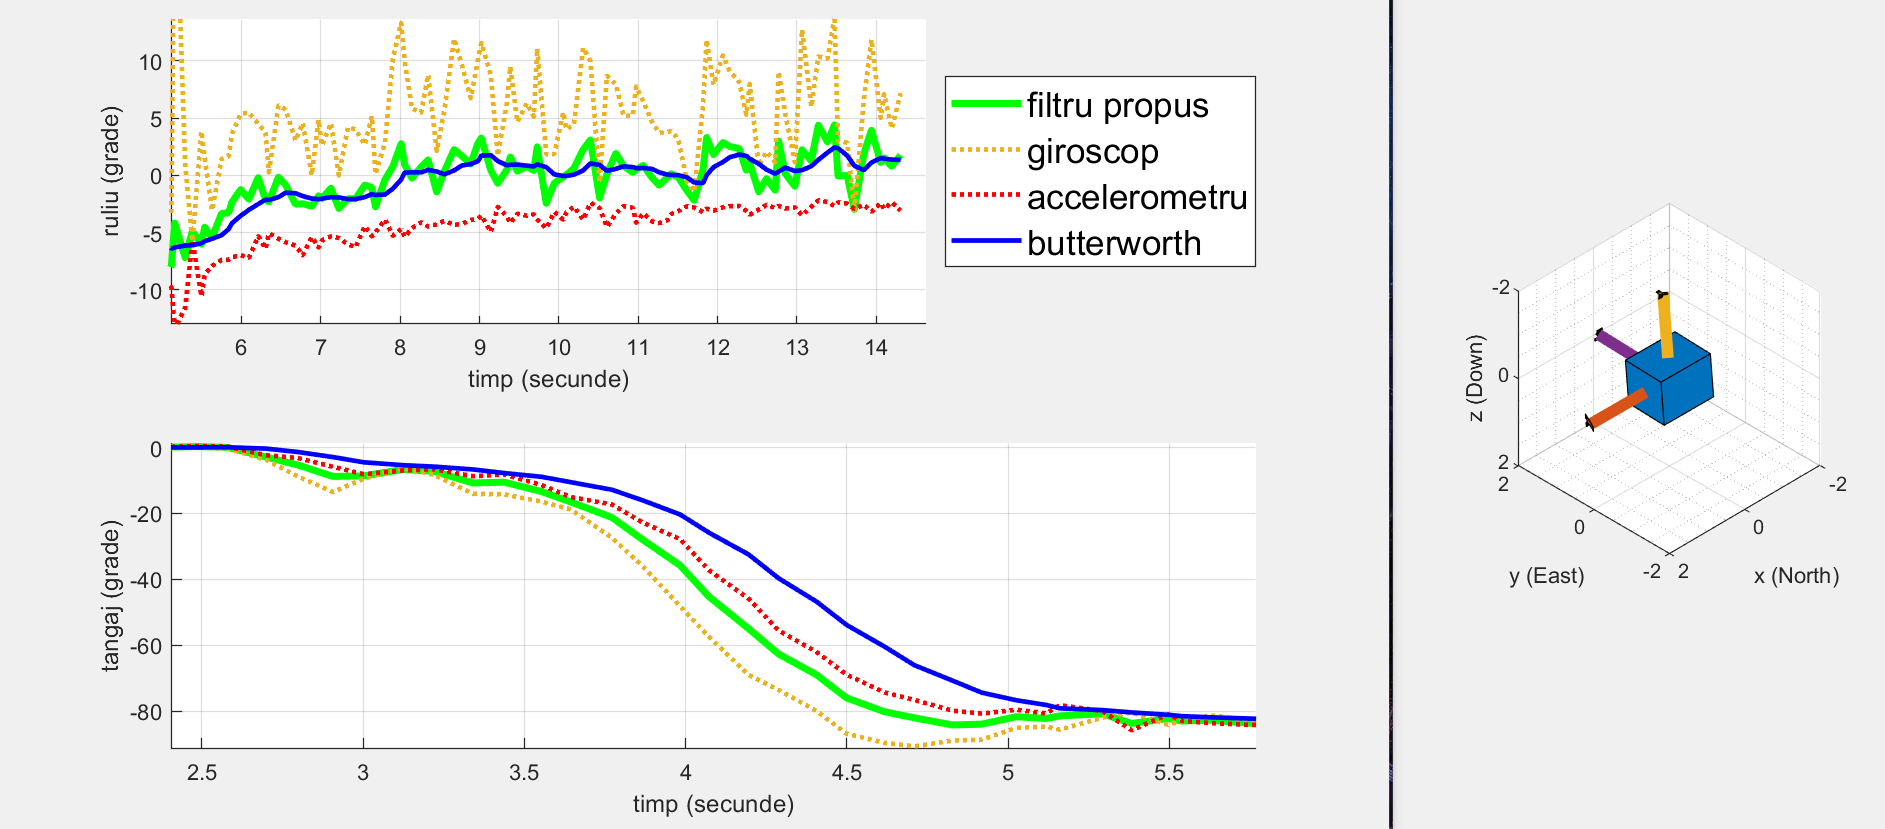
\includegraphics[width=150mm,height=70mm,]{img/Pitch}
 \caption{Fuziunea senzorial'a prin Kalman comparat'a cu m'asur'atorile individuale}
\end{figure}

Pentru a reduce 'si mai mult eroarea, un filtru Butterworth \cite{butter} de tip trece jos poate fi folosit recursiv pe baza unei func'tii de transfer de ordin I, cu o frecvent'a de t'aiere aleas'a empiric de 10 ori mai mic'a dec\ia frecvent'a nyquist ($f_{nyquist} = f/2 = 100 Hz$). Principalul dezavantaj adus de suplimentarul FTJ este c'a acesta introduce o 'int\ia rziere m'asurabil'a, fapt pe care l-am considerat nefiabil pentru o aplica'tie de timp real, 'si pe care deci nu l-am introdus 'in implementarea final'a. 

\begin{figure}[h]
% \hspace*{-1cm}
\centering
 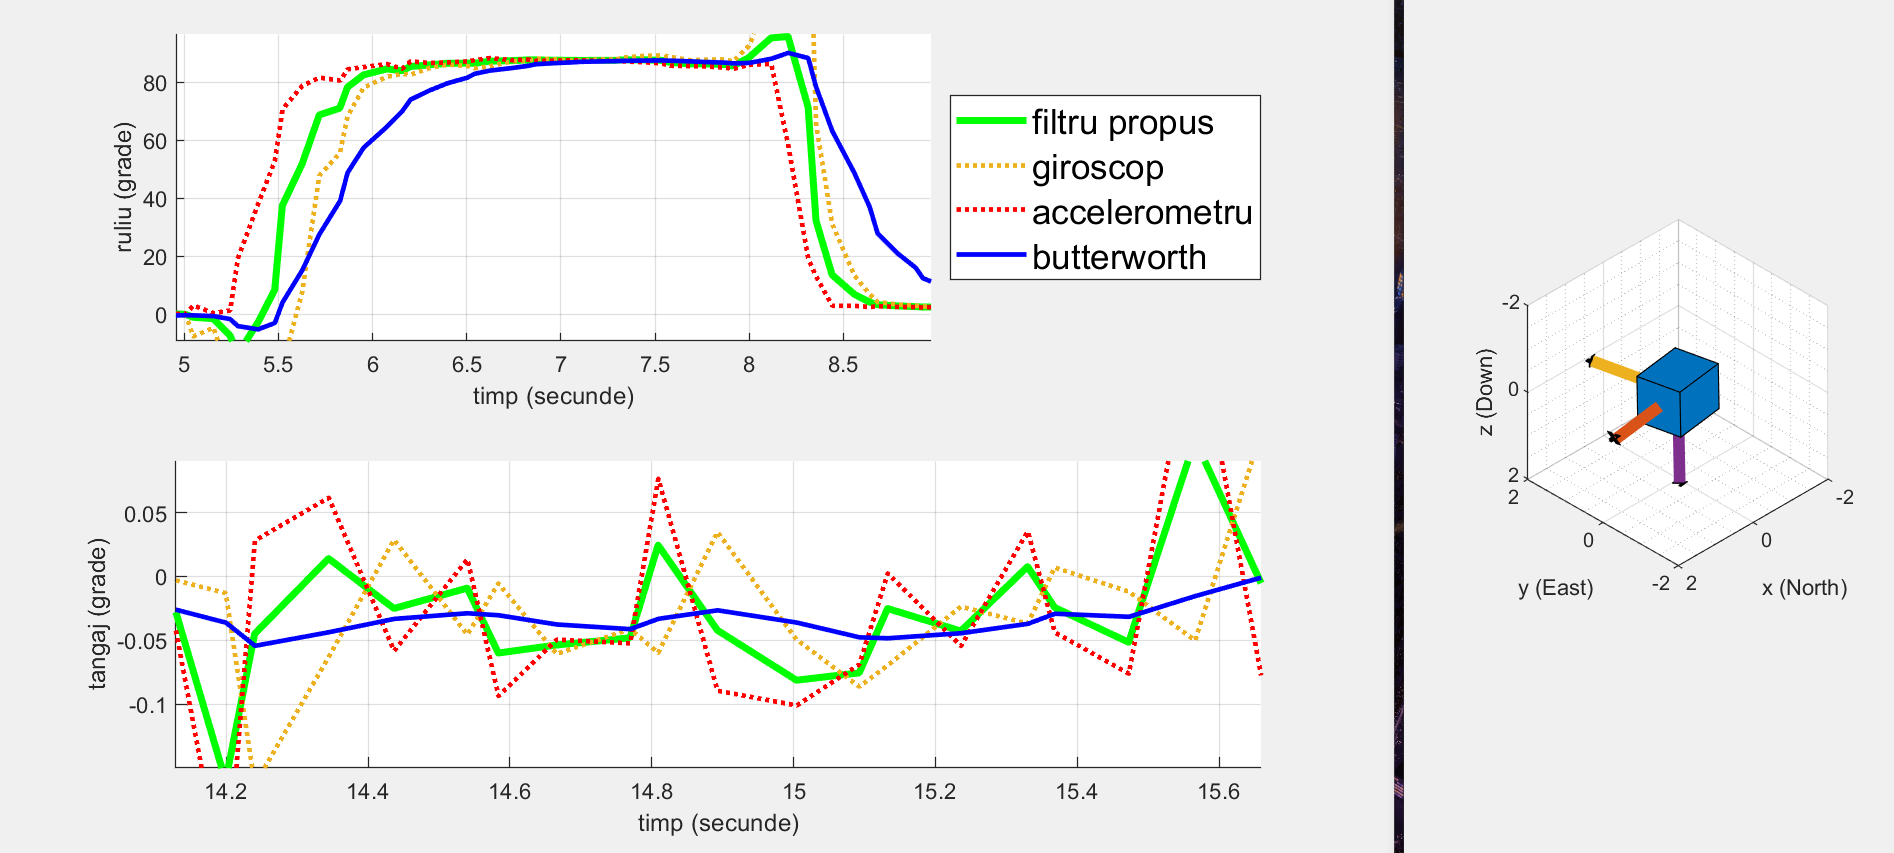
\includegraphics[width=150mm,height=70mm,]{img/Roll}
 \caption{Fuziunea senzorial'a prin Kalman comparat'a cu m'asur'atorile individuale}
\end{figure}

Convergen'ta algoritmului este garantat'a de filtrul liniar pentru ambele unghiuri, 'si estimarea orient'arii func'tioneaz'a 'si 'in regim dinamic, dup'a cum se vede 'in figura 5.4.

\section{Schema general'a de func'tionare}

\begin{figure}[H]
\hspace*{-2.5cm}
% \centering
 \includesvg[width=200mm,height=350mm,scale=1]{img/ObjectTracking}
 \caption{Schema bloc general'a de func'tionare a aplica'tiei}
\end{figure}

% \pagebreak

Schema din figura 5.5 ofer'a o privire de ansamblu asupra scenariului de derulare al jocului. Obiectul ur'arit este controlat prin orientarea pl'acii de dezvoltare ob'tiunit'a prin fuziunea datelor celor doi senzori prezen'ti, 'iar trei metode de estimare sunt posibile 'in func'tie de tipul de mi'scare realizat. Fuziunea este realizat'a conform schemei din figura 5.2, prin algoritmul de fuziune $QKF$ (filtrul Kalman cu cuaternioni) prezentat treptat de la 'inceputul capitolului.

\vspace{5px}

Pentru un proces liniar, filtrul Kalman simplu ($KF$) este de preferat, dar um'arirea se poate realiza 'si prin filtrele extins sau unscented. Acest lucru e posibil pentru c'a 'si obiectul 'in mi'scarea liniar'a dispunde de o vitez'a de rota'tie, doar c'a se consider'a nul'a. Filtrul simplu nu are la dispozi'tie o faz'a de corec'tie bazat'a pe m'asur'atori polare, pentru c'a acestea nu pot fi restr\ia nse la ecua'tii algebrice liniare.  

\vspace{5px}

Pozitia unui obiect relativ'a la cele dou'a axe de mi'scare poate fi transformat'a 'in coordonate polare pentru a intra 'in faza de corec'tie a unuia dintre cele dou'a filtre neliniare, unde m'asur'atorile vor fi comparate cu informa'tia de tip Point Cloud a sonarului, care are mult mai mult'a acurate'te dec\ia t m'asur'atorile de tip GPS primite 'in faza de corec'tie liniar'a. Astfel, at\ia t pentru $EKF$ (filtrul Kalman extins), c\ia t 'si pentru $UKF$ (unscented), fuziunea senzorial'a se realizeaz'a prin aditivitatea celor dou'a faze de corec'tie. Ini'tial, m'asur'atorile de tip GPS confirm'a sau corecteaz'a eroarea estim'arii ob'tinute prin propagarea procesului modelului, dup'a care 'si mai fiabilele m'asur'atori ale sonarului au o interven'tie 'in algoritm. 

\vspace{5px}

'In faza de predic'tie a fitrelor neliniare, pot fi primite m'asur'atori ale vitezei unghiulare zgomotoase de la giroscop pentru modelare, dar nu este imperios necesar, deorece aceast'a m'arimea poate fi modelat'a ca zgomot de proces, a'sa cum este 'si accelera'tia. Se realizeaz'a astfel trei algoritmi de estimare 'in bucl'a 'inchis'a, ale caror erori de estimare sunt ob'tinute prin compararea cu adev'arul prin ceea ce e reprezentat schematic ca \textit{monitorizare}, iar aceast'a eroare devine intrarea ponderat'a 'in dinamica procesului urm'aritor.

\vspace{5px}

Filtrul unscented este cel mai complex algoritm prezent 'in aplica'tie, deoarece a necesitat 'in plus dou'a func'tii de calculare a punctelor sigma 'si a ponderilor lor (explicate 'in capitolul precedent), iar acesta poate fi contruit fie pe baza aceluia'si model de proces folosit 'si pentru filtrul extins, fie pe baza unuia modificat, dup'a cum se va vedea.

\vspace{5px}

Am considerat procesul urm'aritorului ca fiind liniar pentru toate cazurile de mi'scare, pentru ca astfel s'a se poat'a aplica fie metoda de alocare a polilor schi'tat'a 'in figur'a, fie prin reglare liniar - p'atratic'a. Un punct de dezolvatare viitor care rezult'a de aici este explorarea metodelor de control neliniare 'in vederea ob'tinerii unor rezultate mai aproape de adev'ar. 

\vspace{5px}

Rezultatul final al algoritmul, 'si implicit obiectivul proiectului propus este convergen'ta st'arilor urm'aritorului la valorile de stare ale obiectului urm'arit. Astfel se realizeaz'a o urm'arire de traiectorie complet autonom'a, f'ar'a interven'tia utilizatorului, iar 'in restul capitolului voi explica implementarea programatic'a activ'a a cumulului de no'tiuni teoretice prezentate 'in capitolul dedicat analizei teoretice.

\section{Diagrama claselor}

\begin{figure}[H]
\hspace*{-1cm}
% \centering
 \includesvg[width=180mm,height=250mm,scale=1]{img/OOP}
 \caption{Diagrama claselor folosite 'in aplica'tie}
\end{figure}


Figura 5.6 prezint'a totalitatea claselor implementate 'in MATLAB pe care le-am considerat necesare realiz'arii jocului. Abstractizarea obiectivului prin obiecte 'si clase a fost inspirat'a de proiectul \cite{AKSF}. Folosind structurile POO (programare orientat'a pe obiecte) puse la dispozi'tie de limbajul de programare am coceput trei scenarii posibile de urm'arire simulate: mi'scare liniar'a, circular'a 'si aleatorie, iar cel mai 'inalt grad al performan'tei este scenrariul mi'sc'arii comandate de utilizator, care se poate prezenta ca o combina'tie dintre celelalte trei.

\vspace{5px}

Astfel, prin mo'stenire direct'a, toate clasele au acces la metodele superclasei \textit{handle} \cite{handle}. Aceast'a clas'a unic'a din limbaj este necesar'a pentru referirea, 'stergerea sau modificarea instan'telor unei clase, 'si astfel este indispensabil'a model'arii dinamicii obiectelor 'in timp. Aceast'a rela'tie de mo'stenire este de altfel singura leg'atur'a 'intre clase, 'intruc\ia t am inten'tionat func'tionarea lor independent'a 'in func'tie de scenariul ales.

\vspace{5px}

A'sadar, cele trei varia'tiuni ale filtrului Kalman analizate 'in capitolul precedent se reg\ia sesc 'in cele trei clase \textit{KalmanFilterModel}, \textit{ExtendedKalmanFilterModel} 'si \textit{UnscentedKalmanFilterModel}. Fiecare dintre filtre a fost implementat pentru a estima un model de mi'scare diferit, iar 'in acest sens am implementat cele trei clase \textit{VehicleModel2D}, \textit{ExtendedVehicleModel2D} 'si \textit{UnscentedVehicleModel2D}. 

\vspace{5px}

Prima dintre cele trei modeleaz'a dup'a cum se observ'a 'si din atribute (numite propriet'a'ti 'in MATLAB) cazul de mi'scare liniar'a 'si poate fi estimat'a cu succes de toate cele trei filtre. At\ia t modelul extins, c\ia t 'si modelul unscented descriu mi'scarea neliniar'a sub un unghi a obiectului 'si singura diferen't'a dintre cele dou'a este admisia zgomotului pentru intr'arile procesului unscented (accelera'tia 'si viteza unghiular'a). Am inten;tionat 'in acest fel s'a creez o estimare mai robust'a at\ia t la zgomotele reale provenite de la senzor c\ia t 'si la cele simulate 'in aplica'tie. Cu toate aceastea, modelul extins este suficient pentru ambele filtre neliniare, pentru c'a se bazeaz'a pe acela'si vector de stare. 

\vspace{5px}

Pentru fuziunea senzorial'a a datelor de la giroscop 'si accelerometru demonstrat'a la 'inceputul capitolului am implementat clasa \textit{QuaternionKalmanFilterModel} care implementeaz'a ecua'tiile de transformare 'si propagare a dinamicii orient'arii prezentate 'in (4.178) - (4.192) 'si (5.2) - (5.9) pentru modelul procesului giroscopului, 'si corec'tia prin unghiurile de 'inclina'tie ob'tinute din datele accelerometrului reg'asite 'in (5.10) - (5.20). 

\vspace{5px}

Toate clasele construite sunt instan'tiate 'intr-un script (cod) principal care 'ini'tiaz'a 'si 'intre'tine 'si anima'tia, dup'a cum se va vedea 'in continuarea capitolului. Scriptul principal 'in MATLAB nu este o clas'a, 'si deci nu se reg'ase'ste 'in diagrama din figura precedent'a, dar func'tiile folosite sunt demne de explicat pentru a contura contextul programatic al aplica'tiei, 'si nu numai cel 'stiin'tific.

\vspace{5px}

Acest script principal este responsabil de asemenea de realizarea controlului urm'aritorului, obiect care va fi mereu o instan't'a a clasei \textit{VehicleModel2D}, 'intruc\ia t procesul s'au este modelat liniar. Tot aici are loc 'si generarea graficelor de perfomant'a care vor fi puse la dispozi'tie 'in capitolul ~\ref{ch:testing}, iar implementarea structurilor de estimare pe clase faciliteaz'a comparat'ia st'arilor pentru o analiz'a 'in detaliu a erorilor. 

\section{Diagrama de flux}

\begin{figure}[H]
% \hspace*{-1cm}
\centering
 \includesvg[width=180mm,height=200mm,scale=1]{img/Flux}
 \caption{Diagrama fluxului de execu'tie al programului}
\end{figure}

Execu'tia sistematic'a a aplica'tiei 'in mai multe etape este prezentat'a 'in figura 5.7. Porgramul se desf'asoar'a ca un joc, cu o interfa't'a grafic'a specific'a, din care utiliziatorul poate alege scenariul urm'aririi (traiectoria mi'sc'arii) 'si nivelul de dificultate (algoritumul de estimare). 'In caz c'a placa de dezvoltate nu este conectat'a, jocul ruleaz'a ca o simulare 'in care se pot explora performan'tele fiec'arui filtru.

\vspace{5px}

Modul de dezvoltare (\textit{developer}) porne'ste script-ul f'ar'a interfa'ta grafic'a, 'si rolul lui este de a oferi o configura'tie proprie simul'arii, 'in vederea acord'arii filtrelor. Astfel, pentru modelul liniar, se pot seta st'arile ini'tiale ale procesului astfel 'inc\ia t s'a fie fiabile 'si pentru procesul neliniar:

\begin{equation}
    x_0 = \begin{bmatrix}
    p_{x_0} & p_{y_0} & v_{0} & \beta_{0} 
    \end{bmatrix}
\end{equation}

de unde se recupereaz'a vitezele pentru cele dou'a axe:

\begin{gather}
    v_x = \cos{\beta_0} \times v_0 \\
    v_y = \sin{\beta_0} \times v_0
\end{gather}

De notat este c'a unghiul $beta$ setat la 'inceput este unghiul sub care se va desf'a'sura mi'scarea liniar'a, 'insemn\ia nd c'a acesta nu se mai modific'a pe parcursul traseului, iar dinamica lui este constant'a. Pentru st'arile prelucrate se pot seta abaterile standard:

\begin{equation}
    \sigma = \begin{bmatrix}
    \sigma_{p} & \sigma_{v} & \sigma_{a} & \sigma_{m}
    \end{bmatrix}
\end{equation}

unde, pentru simplificare, abaterea standard a ambelor pozi'tii 'si cea a ambelor viteze sunt evaluate cu c\ia te o valoare. Devia'tia ambelor accelera'tii este 'inglobat'a 'in $\sigma_{a}$, iar $\sigma_{m}$ reprezint'a abaterea m'asur'atorilor primite de la GPS. 

\vspace{5px}

Am configurat 'si un steag cu valoare boolean'a care stabile'ste dac'a filtrul va fi initializat cu stare $x_0$ a procesului, sau dac'a acesta nu de'tine cuno'stiinte a priori despre proces. 'In ambele cazuri, filtrul liniar va converge. Acela'si steag controleaz'a 'si ini'tializarea parametrilor urm'aritorului. Astfel, matricea de covarian't'a a st'arii se programez'a:

\begin{gather}
\centering
    P = \begin{bmatrix}
     \sigma^2_{m} & 0 & 0 & 0 \\ 0 & \sigma^2_{m} & 0 & 0 \\ 0 & 0 &  \sigma^2_{v} & 0 \\ 0 & 0 & 0 & \sigma^2_{v} 
    \end{bmatrix} sau \hspace{5px}
     P = \begin{bmatrix}
     \sigma^2_{p} & 0 & 0 & 0 \\ 0 &  \sigma^2_{p} & 0 & 0 \\ 0 & 0 &  \sigma^2_{v} & 0 \\ 0 & 0 & 0 & \sigma^2_{v} 
    \end{bmatrix}
\end{gather}

'in func'tie de setarea steagului. Zgomotul de proces $Q$ 'inglobeaz'a dinamica celor dou'a accelera'tii primite ca intr'ari 'in proces 'si este initializat ca 'in (4.47) folosind varian'ta accelera'tiei (p'atratul abaterii, considerat identic pentru ambele axe spre simplificare) 'in locul accelera'tiilor propriu zise. Zgomotul de m'asur'a $R$ va depinde mereu de varian'ta m'asur'atorilor de tip GPS:


\begin{equation}
    R = \begin{bmatrix}
     \sigma^2_{m} & 0 \\ 0 & \sigma^2_{m}
    \end{bmatrix}
\end{equation}

Componentele vectorului de accelera'tie sunt setate stocastic cu fun'ctia MATLAB $randn$ \cite{randn} ce returneaz'a numere aleatorii distribuite Gaussian, folosit'a 'si pentru a genera zgomotul ce afecteaz'a m'asur'atorile exacte ale pozi'tiilor victimei, ce devin intr'arile func'tiei de corec'tie (4.86) - (4.87). At\ia t vectorul de stare c\ia t 'si matricea de covarian't'a sunt rescrise recursiv 'in ambele etape ale algoritmului 'si astfel se realizeaz'a o estimare'in bucl'a 'inchis'a conform fazelor de predic'tie  (4.85) 'si corec'tie a filtrului liniar (4.106) - (4.113). Modelul procesului liniar, dar 'si cel al urm'aritorului sunt bazate pe legile de mi'scare (4.44) - (4.45), scrise matricial ca 'in (4.162) - (4.163).  

\vspace{5px}

Faza de predic'tie a procesului extins con'tine 'in plus informa'tii despre varian'ta vitezei de gira'tie a victimei. Pentru a face algoritmul mai eficient, am inclus o modificare a m'asur'atoarii giroscopului de pe axa X (prin care va comanda juc'atorul gira'tia propriu-zis'a) pentru care am ad'augat zgomot alb, deci se poate considera c'a filtrul prime'ste informa'tie 'in plus de la giroscop. Din moment ce algoritmul neliniar e vulnerabil la divegent'a, am considerat obligatorie op'tiunea de ini'tializare a filtrului cu primele m'asur'atori, de'si este demn de mne'tionat c'a 'intr-un scenariu real acest lucru nu este mereu posibil. Astfel, am ini'tializat matricea de covarian't'a. 

\begin{equation}
    P = \begin{bmatrix}
     \sigma^2_{m} & 0 & 0 & 0 \\ 0 & \sigma^2_{m} & 0 & 0 \\ 0 & 0 &  \sigma^2_{\beta} & 0 \\ 0 & 0 & 0 & \sigma^2_{v} 
    \end{bmatrix}
\end{equation}

Prin liniarizarea distribu'tiei zgomotului de proces (4.77), noua varian't'a celor dou'a intr'ari - viteza de gira'tie 'si accelera'tia poate fi 'inglobat'a astfel (4.114), (4.130) \cite{AKSF}: 

\begin{equation}
    Q = \begin{bmatrix}
     0& 0 & 0 & 0 \\ 0 & 0 & 0 & 0 \\ 0 & 0 & \Delta t^2  \sigma^2_{\dot \beta} & 0 \\ 0 & 0 & 0 & \Delta t^2 \sigma^2_{a} 
    \end{bmatrix}
\end{equation}

Faza de corec'tie liniar'a func'tioneaz'a ca 'in cazul precedent, iar ad'augarea sonarului este optional'a, pentru acesta model\ia ndu-se un zgomot de m'asur'a $R_{extins}$:

\begin{equation}
    R_{extins} = \begin{bmatrix}
     \sigma^2_{r} & 0 \\ 0 & \sigma^2_{\gamma}
    \end{bmatrix}
\end{equation}

iar algoritmul decurge 'in continuare conform ecua'tiilor (4.128) - (4.141). 

\vspace{5px}

Pentru filtrul Kalman unscented, vectorul de stare se poate augmenta asstfel 'inc\ia t s'a con'tin'a 'si informa'tie at\ia t despre cele patru abateri ale st'arilor, c\ia t 'si despre abaterile celou dou'a m'asur'atori neliniare de raz'a 'si unghi oferite de sonar:

\begin{equation}
    X_{aug} =  [X, \nu_{p_x}, \nu_{p_y}, \nu_{\dot \beta}, \nu_{a}, \omega_r, \omega_\gamma]
\end{equation}

unde $\nu$ 'si $\gamma$ reprezint'a zgomotul de proces, respectiv m'asur'a. 

\vspace{5px}

Se ob'tine astfel un vector augmentat ce con'tine 10 st'ari, care este trecut prin transformata unscented (4.142), iar covarian'ta lui este construit'a prin augmentarea matricei anterioare P astfel: 

\begin{equation}
    P_{aug} = \begin{bmatrix}
    P & 0 & 0 \\ 0 & Q & 0 \\ 0 & 0 & R
    \end{bmatrix}
\end{equation}

'si aceasta este propagat'a conform (4.143), unde punctele $\sigma$ 'si ponderile au fost calculate conform (4.150) - (4.153) pentru 20 de valori. Pentru faza de corec'tie neliniar'a, dac'a este prezent'a, matricea de covarian'ta augmentat'a se rescrie astfel 'inc\ia t s'a 'inglobeze incertitudinea m'asur'atorilor sonarului: 

\begin{equation}
    P_{aug} = \begin{bmatrix}
    P & 0 & 0 \\ 0 & Q & 0 \\ 0 & 0 & R_{extins}
    \end{bmatrix}
\end{equation}

'si func'tia de generare a punctelor sigma este apelat'a din nou, dar nu 'si cea a ponderilor, care, conform (4.152) - (4.153) r'am\ia n constante pe parcursul estim'arii. Filtrul parcurge toate etapele (4.154) - (4.161). Sonarul este ales static pentru un punct de observare fix 'in raport cu care se m'asoar'a raza 'si unghiul obiectului urm'arit pentru fiecare itera'tie.

\vspace{5px}

Se observ'a  cum transformata unscented introduce complexitate 'in plus pentru calcularea ponderilor 'si punctelor $\sigma$, buclele de calcul devenind $\mathcal{O}(20n)$. Motivul pentru care cele 10 st'ari ale vectorului agumentate sunt dublate este oglindirea parametrilor conform figurii (4.13) 'in vederea recuper'arii noii elipse de covarian't'a. Pentru aplica'tia prezent'a de tip joc, aceast'a compelxitate este neglijabil'a 'in raport cu num'arul de itera'tii folosite pentru fiecare mi'scare, 'si filtrul unscented devine o op'tiune avantajoas'a pentru unele dintre scenarii. 

\vspace{5px}

Dinamica anima'tiei depinde de perioada de e'santionare, 'si acesta este 'si motivul pentru care procesul continuu teoretizat la 'inceputul capitolului precedent nu poate fi integrat 'intr-o aplica'tie de acest fel, cum de altfel 'si procesele 'inglobate pe sisteme de calcul sunt mereu discrete. Astfel, perioada de e'santionare 'si frecven'ta de resetare a anima'tiei au fost alese empiric 'tin\ia nd cont de urm'atoarea regul'a:

\begin{equation}
    \frac{1}{f} < pause < \Delta t 
\end{equation}

unde $f$ reprezint'a frecvent'a datelor de citire de la senzorul real MPU-6050, iar $pause$ perioada de pauz'a dintre cadre. 'In acest fel, se asigur'a o tranzi'tie neted'a de la comanda joystick-ului la anima'tie, care la r\ia ndul ei permite observarea desf'a'sur'arii dinamicii procesului 'si a urm'ariltorului. 'In figurile 5.8 - 5.10 se pot observa diferitele scenarii 'in ac'tiune.

\begin{figure}[h]
    % \centering
    \hspace*{-3cm}
    \subfloat[\centering Estimarea pozi'tiei]{{\includesvg[width=100mm]{img/thisone}}}%
    \qquad
    \subfloat[\centering Convergen'ta autonom'a]{{\includesvg[width=100mm]{img/lincatch} }}%
    \caption{Urm'arirea traiectoriei liniare}%
    % \label{fig:example}%
\end{figure}


\begin{figure}[h]
    % \centering
    \hspace*{-3cm}
    \subfloat[\centering Estimarea pozi'tiei]{{\includesvg[width=100mm]{img/circchase}}}%
    \qquad
    \subfloat[\centering Convergen'ta autonom'a]{{\includesvg[width=100mm]{img/circular} }}%
    \caption{Urm'arirea traiectoriei circulare}%
    % \label{fig:example}%
\end{figure}


\begin{figure}[H]
    % \centering
    \hspace*{-3cm}
    \subfloat[\centering Estimarea pozi'tiei]{{\includesvg[width=100mm]{img/randchase}}}%
    \qquad
    \subfloat[\centering Convergen'ta autonom'a]{{\includesvg[width=100mm]{img/random} }}%
    \caption{Urm'arirea traiectoriei aleatorii}%
    % \label{fig:example}%
\end{figure}

% 'Impreun'a cu capitolul precedent reprezint'a aproximativ 60\% din total.

% Scopul acestui capitol este de a documenta aplica'tia dezvoltat'a 'in a'sa fel 'inc\ia t dezvoltarea 'si 'intre'tinerea ulterioar'a s'a fie posibile. 
% Cititorul trebuie s'a identifice func'tiile principale ale aplica'tiei din ceea ce este scris aici.
% Capitolul ar trebui sa con'tin'a (nu se rezum'a neap'arat la):
% \begin{itemize}
%  \item schema general'a a aplica'tiei
% \item descrierea fiec'arei componente implementate, la nivel de modul
% \item diagrame de clase, clase importante 'si metode ale claselor importante.
% \end{itemize}


\chapter{Testare 'si Validare}
\label{ch:testing}

Pentru dinamica estimatorului, a procesului victim'a 'si a urm'aritorului sunt salvate vectorial st'arile 'in fiecare moment de timp, 'si astfel, la finalul jocului, atunci c\ia nd rechinul prinde foca (prin epuizarea punctelor ro'sii de viat'a), se pot trage concluzii asupra performan'tei urm'aririi. Aceste grafice au fost folosite pentru a decide nivelul de acordare suplimentar cerut de regulator sau de filtru. 


\begin{figure}[h]
\hspace*{-5cm}
% \centering
 \includesvg[width=230mm,height=150mm,scale=1]{img/lin_performance}
 \caption{Evaluarea performantelor procesului liniar}
\end{figure}

Se poate observa 'in figura 6.1 cum st'arile estimatorului converg la cele reale ale procesului, respectiv cum st'arile urm'aritorului converg prin control la estim'arile f'acute de filtru. Pentru ambele pozi'tii, at\ia t estim'arile c\ia t 'si reglarea sunt mai aproape de adev'ar dec\ia t m'asur'atorile zgomotoase, ceea ce 'inseamn'a c'a algoritmul 'si-a 'indeplinit obiectivul. 

\vspace{5px}

Mai mult, dup'a cum se vede 'in ultimele 4 figuri, erorile de estimare ale fiec'arei st'ari converg la 0, 'si sunt 'inglobate de incertidudinea de $\pm 3 \sigma$ a devia'tiei standard rezultate din extragerea radicalului varian'tei. Pentru fiecare faz'a de predic'tie incertitudinea din proces este crescut'a de zgomotul de proces $Q$, conform (4.85), pentru ca mai apoi s'a fie 'intre'tinut'a prin faza de corec'tie (4.113). 'In acest exemplu, covarian'ta st'arilor nu este minimizat'a, ci r'am\ia ne aproximativ constant'a din cauza noilor incertiduni ap'arute 'in proces, dar at'at st'arile, c\ia t 'si erorile converg, ceea ce 'inseamn'a c'a filtrul liniar are succes. 

\begin{figure}[h]
\hspace*{-4cm}
% \centering
 \includesvg[width=230mm,height=150mm,scale=1]{img/input_linear}
 \caption{Evaluarea performantelor procesului liniar}
\end{figure}

Figura 6.2 prezint'a pe de o parte inova'tia (eroarea) m'asur'atorilor de tip GPS admise 'in faza de corec'tie, care poate fi 'incadrat'a 'in gama mai strict'a de $\pm \sigma$ (o devia'tie standard) prev'azut'a 'inainte de rularea aplica'tiei. Important'a pentru distribu'tia erorilor este 'si media cu valoare nul'a, iar acest lucru se transpune 'si 'in intrarea dat'a regulatorului ce comand'a mi'scarea rechinului. Astfel, comanda dat'a este capabil'a s'a mimeze forma distribu'tiei accelerat'iei adev'arate ale victimei de pe ambele axe, dar cu o varian't'a observabil mai mare, ceea ce 'insemn'a c'a efortul depus de rechin pentru a prinde foca este semnificativ, iar o astfel de comand'a ar putea s'a nu fie fiabil'a pentru un regulator real. Se poate nota de asemenea cum 'inainte de convergent'a general'a, eroarea din proces tinde s'a creasc'a, p\ia n'a c'and informa'tia primit'a prin m'asur'atori este evaluat'a.

\vspace{5px}

Accelera'tia pentru acest experiment a fost setat'a cu o valoare neglijabil'a 'in raport cu pozi'tia 'si viteza ini'tial'a, 'si de accea pozi'tia cres'te aproximativ liniar, iar viteza r'am\ia ne constant'a. Pentru o dinamic'a mai complex'a 'ins'a, performan'tele algoritmilor se diversific'a, dup'a cum va fi eviden'tiat 'si 'in experimentele urm'atoare.

\vspace{5px}

Un caz de mi'scare circular'a este prezentat 'in figura 6.3, pentru care filtrul Kalman extins doar cu o faz'a de corec'tie liniar'a a fost folosit ca estimator. O astfel de mi'scare presupune o schimbare continu'a vitezei 'si a gira'tiei, 'si se poate observa cum 'si incertidunea din proces pentru pozi'tii se modific'a din cauza neliniarit'a'tiilor introduse. Se vede cum 'in acest caz faza de maximizare (predic'tie), respectiv cea de minimizare (corec'tie) a covarian'tei modific'a vizibil forma distribu'tiei 'in timp. Orientarea poate fi estimat'a cu succes datorit'a informa'tiei despre rata de gira'tie a procesului integrat'a 'in faza de predic'tie a modelului, iar varian'ta vitezei r'am\ia ne constant'a din cauza stocasticit'a'tii accelera'tiei necesar'a producerii virajelor.

% \begin{figure}[h]
% \hspace*{-5cm}
% % \centering
%  \includesvg[width=230mm,height=150mm,scale=1]{img/accelerated_lin}
%  \caption{Evaluarea performantelor procesului liniar}
% \end{figure}

\begin{figure}[h]
\hspace*{-5cm}
% \centering
 \includesvg[width=230mm,height=150mm,scale=1]{img/ekf_performance}
 \caption{Filtrul Kalman extins pentru o traciectorie circular'a}
\end{figure}

Pentru a limita intervalul valabil pentru atitudinea procesului victim'a am folosit func'tia MATLAB \textit{wrapTo180} \cite{wrap} , 'si astfel de ficare dat'a c\ia nd se termin'a un cerc complet de mi'scare se poate observa pe grafic o linie vertical'a. Pozi'tiile axelor X 'si Y vor echivala cu func'tiile cosinusoid'a, respectiv sinusoid'a dependente de magnitudinea  accelera'tei. 

\vspace{5px}

'Imbun'at'a'tirea major'a introdus'a de ad'augarea fazei de corec'tie neliniare se observ'a 'in figura 6.4 'in primul r\ia nd pentru acurate'tea suplimentar'a reg'asit'a 'in estimarea orient'arii. Nu numai c'a estimarea are o convergen't'a mai neted'a 'si mai rapid'a, dar 'si varian'ta m'asur'atorii este minimizat'a considerabil prin introducerea noului senzor. Conform ecua'tiilor fazei de corec'tie extinse (4.137) - (4.141), se poate observa c'a matricea de covarian'ta este minimizat'a indiferent de convergen'ta vectorului de stare, ceea ce 'inseamn'a c'a at\ia t execu'tia algoritmului, c\ia t 'si acordarea a priori au fost de succes.

\vspace{5px}

'Si de aceast'a dat'a fazele succesive de maximizare, respectiv minimizare ale varian'telor pozit'iilor pot fi obsevate mai clar 'in cele dou'a grafice, fa't'a care estimarea converge independent cu mai put'in'a incertidune la stare. Modelul procesului urm'aritorului este 'in continuare unul liniar, 'si de aceea performan'tele lui nu sunt comparate pentru noile st'ari prezente 'in figur'a, ci dec\ia t pentru st'arile de interes final, pozi'tiile, pentru care se observ'a din nou o apropiere mai bun'a dec\ia t cea ob'tinut'a de m'asur'atorile neprocesate. 


\begin{figure}[h]
\hspace*{-5cm}
% \centering
 \includesvg[width=230mm,height=150mm,scale=1]{img/ekf_lidar}
 \caption{Filtrul Kalman extins+ SoNAR pentru o traciectorie circular'a
 }
\end{figure}

Orientarea 'si viteza par s'a fie estimate la fel de bine 'si f'ar'a ajutorul SoNAR-ului, dar, la o privire mai atent'a, se poate constata c'a 'in al figura de sus doar o singur'a linie vertical'a este prezent'a 'in graficul atitudinii, fa't'a de cele dou'a din graficul precedent. Acest lucru 'inseamn'a ca foca a reus'it s'a efectueze un singur cerc complet 'inainte s'a piard'a toate punctele de viat'a prin prindere (convergen'ta estimatorului 'si a regulatorului), fa't'a de cele recordul anterior de dou'a rota'tii complete.

\begin{figure}[h]
\hspace*{-5cm}
% \centering
 \includesvg[width=230mm,height=150mm,scale=1]{img/ekf_lidar_input}
 \caption{Filtrul Kalman + SoNAR extins pentru o traciectorie circular'a
 }
\end{figure}

Probabil cea mai pertinent'a concluzie poate fi tras'a prin analizarea figurii 6.5, unde, cu ajutorul celor patru grafice de performan't'a, se observ'a cum distribu'tia comenzii regulatorului o imit'a aproape perfect pe cea real'a a accelera'tiei aleatorii a procesului. De aici rezult'a c'a rechinul nu depune un efort considerabil mai mare dec\ia t este necesar pentru a prinde foca, iar graficele din st\ia nga figurii 'int'aresc 'si mai mult aceast'a convingere prin expunerea erorilor. Inova'tia m'asur'atorilor este 'si de aceast'a dat'a zero-centric'a, distribuit'a Gaussian, 'ins'a chiar mai mult, 'in plus fa't'a de rezultatul anterior, ea se reg'ases'te foarte strict sub limita procesat'a 'in matricea $S$ a covarian'tei erorilor, calculat'a prin considera'tia ini'tial'a a zgomotului de m'asur'a $R$. Acest aspect relev'a rolul vital jucat de m'asur'atorile exacte ale unui sonar comparativ cu cele foarte zgomotoase ale unui senzor de tip GPS 'in cre'sterea acurate'tii estim'arilor.

\vspace{5px}

Acest scenariu este probabil unul dintre cele mai bune care pot fi ob'tinute pentru o traiectorie neliniar'a, 'ins'a procesul este 'in continuare deterministic prin natura sa, chiar dac'a factorii structurali sunt stocastici. Un experiment mai aproapiat de realitate trebuie s'a permit'a mi'sc'arii neliniare s'a ias'a din repetitivitatea rotirii 'in cerc. 

\vspace{5px}

Am simulat un astfel de model de mi'scare pentru figura 6.6, unde se poate observa c'a orientarea obiectului nu mai este liniar'a nici m'acar pe p'arti, 'si tocmai de aceea am ales s'a aplic transformata unscented estimatorului. Pentru c'a filtrele neliniare nu pot garanta convergen'ta, a trebuit s'a acordez parametrii specific pentru acest tip de mi'scare, ceea ce ar putea 'insemna c'a o structur'a general'a nu poate fi oferit'a pentru toate mi'sc'arile posibile. 

\begin{figure}[h]
\hspace*{-5cm}
% \centering
 \includesvg[width=230mm,height=150mm,scale=1]{img/ukf_lidar}
 \caption{Filtrul Kalman unscented + SoNAR pentru o traciectorie aleatorie
 }
\end{figure}

Dup'a cum se observ'a, valoarea neglijabil'a, cvasinul'a a accelera'tiei determin'a un comportament aproape constant al velocit'a'tii, dar neliniaritatea puternic'a provine din schimb'arile bru'ste de orientare. Acest exemplu nu ar fi convers (nu 'intr-o perioad'a de timp rezonabil'a) f'ar'a interven'tia sonarului 'in faza de corec'tie neliniar'a. 'Tin\ia nd cont c'a modelul mi'sc'arii 'in cauz'a prezint'a cel mai 'inalt grad de stocasticitate, etapele de fluctua'tia ale varian'telor pozi'tiilor sunt 'si mai evidente dec\ia t 'in cazurile precedente. Evident'a 'in acest caz este 'si stabilitatea neclar'a a vitezei estimate comparativ cu cea adev'arat'a, acest lucru fiind datorat cre'sterii zgomotului de proces prin acordarea filtrului.

\begin{figure}[h]
\hspace*{-5cm}
% \centering
 \includesvg[width=230mm,height=150mm,scale=1]{img/ukf_lidar_input}
 \caption{Filtrul Kalman unscented + SoNAR  pentru o traciectorie aleatorie
 }
\end{figure}

La fel de importante sunt 'si concluziile ce se pot trage din graficele puse la dispozi'tie 'in figura 6.7 De'si aspectul Gaussian este recuperat de distribu'tia comenzii regulatorului procesului urm'aritor, distribut'ia 'in sine este mai lat'a, ceea ce denot'a o abatere mai mare a comenzilor fa't'a de medie, f'ac\ia nd controlul dificil de implementat 'in practic'a. De data acesta, erorile m'asur'atorilor de pe axa Y nu au fost bine 'incadrate 'in varian'ta calculat'a pentru inova'tie, iar acest lucru se transpune 'in efortul pe care urm'aritoul 'il depune pentru a prinde victima. Filtrul 'in cauz'a mai are nevoie s'a fie acordat, sau chiar modificat pentru a face fa't'a neliniarit'a'tilor puternice prezente 'in proces. 

\vspace{5px}

Acest ultim exemplu de traiectorie este 'si cel relevant pentru mi'scarea pe care o poate comanda un juc'ator, 'intruc\ia t se a'steapt'a ca aceasta s'a fie oric\ia t de neliniar'a posibil, 'si de aceea, at\ia t prin privirea aspectului teoretic, c\ia t 'si prin demonstra'tiile grafice din acest capitol, consider modelul extins augmentat al filtrului Kalman unscented cel mai fiabil pentru joc 'in sine.  

Pentru algoritmul de fuziune al datelor de la giroscop 'si accelerometru am realizat o compara'tie cu func'tia MATLAB preimplementat'a \textit{imufilter} \cite{imufilter} care porceseaz'a 'si fuzioneaz'a m'asur'atorile celor doi senzori. Am constatat c'a filtrul propriu rezolv'a o problem'a de laten't'a 'in convergent'a estim'arilor. Acest lucru se datoreaz'a faptului c'a func'tia oferit'a de toolbox-ul \textit{Sensor fusion and Tracking} aplic'a un filtru dur rezultatelor pentru a garanta minimizarea erorii de estimare 'in favoarea vitezei.


\begin{figure}[h]
% \hspace*{-1cm}
\centering
 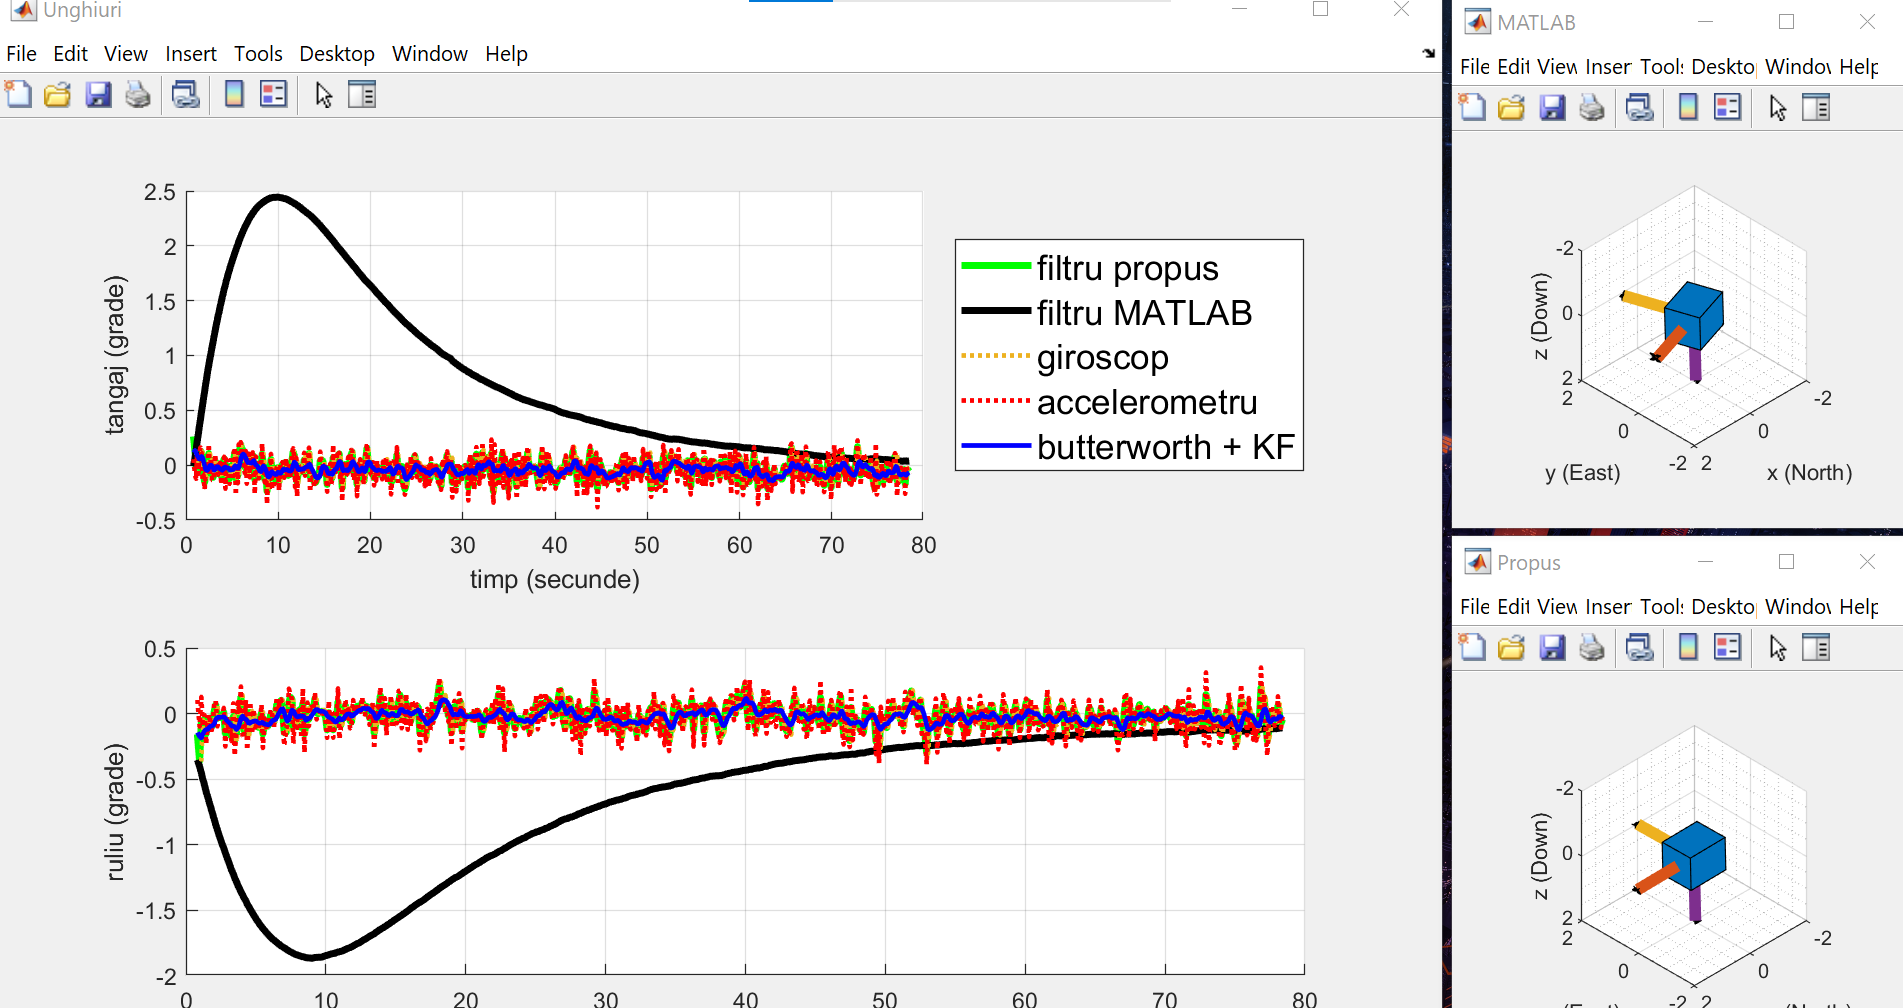
\includegraphics[width=150mm,height=70mm,]{img/compzero}
 \caption{Fuziunea senzorial'a prin Kalman comparat'a cu m'asur'atorile individuale}
\end{figure}

Se poate vedea 'in figura 6.8 cum toate m'asur'atorile senzorului static converg la valoarea de 0, 'ins'a 'in cazul fun'c'tiei \textit{imufilter} acest lucru dureaz'a mai mult de un minut. Acest aspect este desigur inadmisibil pentru o aplica'tie de timp real, cum este 'si cazul jocului dezvoltat,'si de aceea am ales s'a folosesc implementarea proprie. 

\begin{figure}[H]
% \hspace*{-1cm}
\centering
 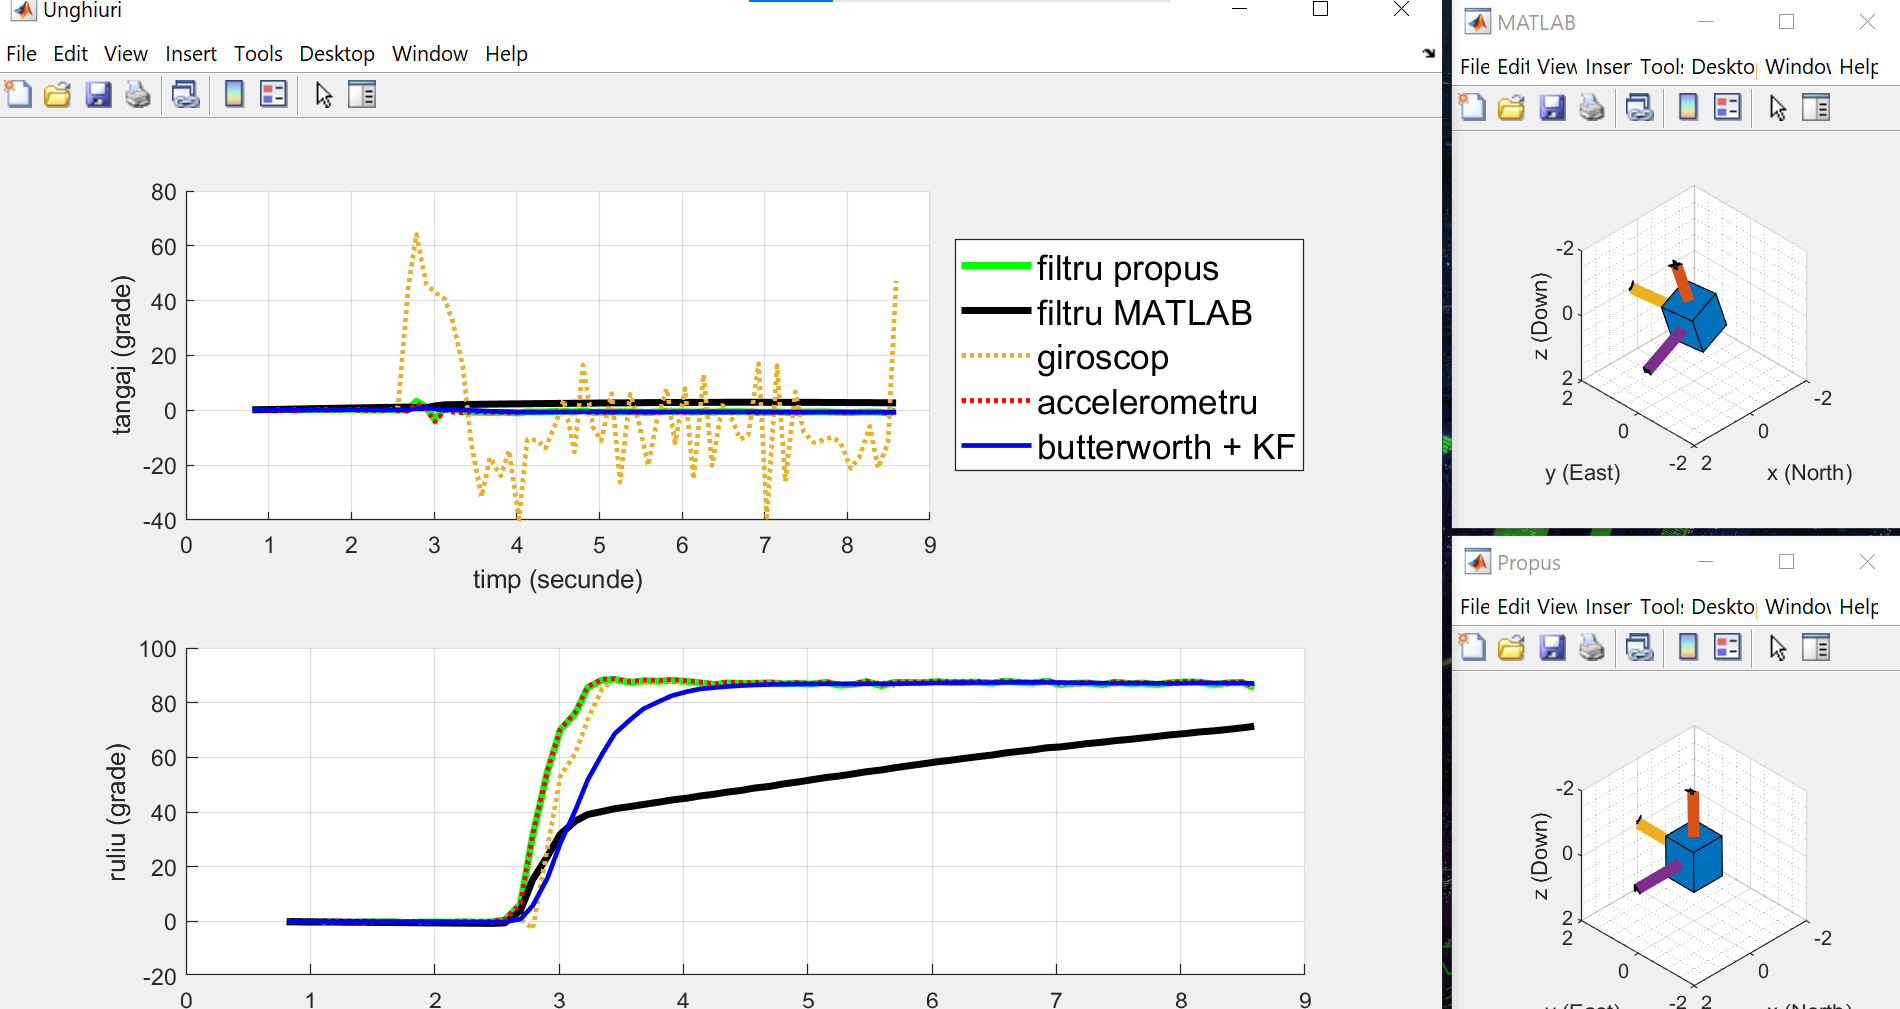
\includegraphics[width=150mm,height=70mm,]{img/comp}
 \caption{Fuziunea senzorial'a prin Kalman comparat'a cu m'asur'atorile individuale}
\end{figure}

Dezavantajul posibil ob'tinut prin propria implementare este c'a f'ar'a un filtru suplimentar, orientarea poate fi gre'sit estimat'a din cauza zgomotului senzorilor. 'In cazul figurii 6.9, se poate observa cum pentru o rota'tie brusc'a pe axa unghiului de ruliu, giroscopul a integrat viteza de rota'tie mare m'asurat'a 'si astfel estim;arile sale sunt eronate pentru axa de tangaj fa't'a de care senzorul era static. Aceast'a problem'a poate fi rezolvat'a prin acordarea unei mai mari 'increderi 'in m'asur'atorile accelerometrului prin diminuarea abaterilor matricei zgomotului de m'asur'a $R$, sau similar prin m'arirea elementelor matricei zgomotului de proces $Q$, ce modeleaz'a erorile giroscopului. Astfel se ob'tine un rezultat satisf'ac'ator, pentru care am aplicat un filtru propriu Butterworth, 'ins'a pe care am ales s'a nu 'il folosesc 'in implementarea final'a, dat'a fiind 'int'arzierea de o secund'a observabil'a 'in figur'a. 

\vspace{5px}


Am comparat concret rezultatele ob'tinute pentru senzorul static cu fiecare metod'a folosind func'tia \textit{immse} \cite{immse} din toolbox-ul de procesare de imagini pus la dispozi'tie de MATLAB 'si am realizat astfel tabelul 6.1. Se poate constata c'a 'intr-aderv'ar, datorit'a filtr'arii suplimentare, func'tia \textit{imufilter} este mai exact'a. 'In afar'a de acest aspect, se poate vedea c'a fuziunea proprie a celor dou'a m'asur'atori independente de la giroscop 'si accelerometru ofer'a o estimare mai pu'tin eronat'a dec\ia t oricare senzor evaluat separat, ceea ce 'insemn'a c'a scopul algoritmului a fost 'indeplinit. 

\begin{table}[ht]
\centering
\begin{tabular}{ |p{6cm}||p{2cm}|p{2cm}|p{2cm}|  }
 \hline
 \multicolumn{4}{|c|}{Eroarea medie p'atratic'a} \\
 \hline
 Metod'a & Faz'a & Ruliu & Tangaj\\
 \hline
 Giroscop - Integrare numeric'a   & Predic'tie    &0.0342&   0.0081\\
 Accelerometru - 'Inclina'tie &  Corec'tie & 0.0373   & 0.0141\\
 Filtru Kalman cuaternioni & Fuziune & 0.0307 &  0.0076\\
 imufilter (MATLAB + toolbox)    & Fuziune & 0.0054&  0.00065\\
 Filtru propus + Butterworth &  Filtru IIR  & 0.0255 & 0.0022\\
 \hline
\end{tabular}
\caption{Analiz'a performan'te}
\label{tab:my_label}
\end{table}


\chapter{Manual de Instalare 'si Utilizare}

% 'In sec'tiunea de Instalare trebuie s'a detalia'ti resursele software 'si hardware necesare pentru instalarea 'si rularea aplica'tiei, precum 'si o descriere pas cu pas a procesului de instalare. 
% Instalarea aplica'tiei trebuie s'a fie posibil'a pe baza a ceea ce se scrie aici.

% 'In acest capitol trebuie s'a descrie'ti cum se utilizeaz'a aplica'tia din punct de vedere al utilizatorului, f'ar'a a men'tiona aspecte tehnice interne.
% Folosi'ti capturi ale ecranului 'si explica'tii pas cu pas ale interac'tiunii. 
% Folosind acest manual, o persoan'a ar trebui s'a poat'a utiliza produsul vostru.

\section{Resurse hardware}

Pentru realizarea joystick-ului au fost folosite un microcontroller Arduino 'in combina'tie cu un modul de senzori MPU-6050 (accelerometru 'si giroscop triaxiale). 


\begin{figure}[h]
% \hspace*{-1cm}
\centering
 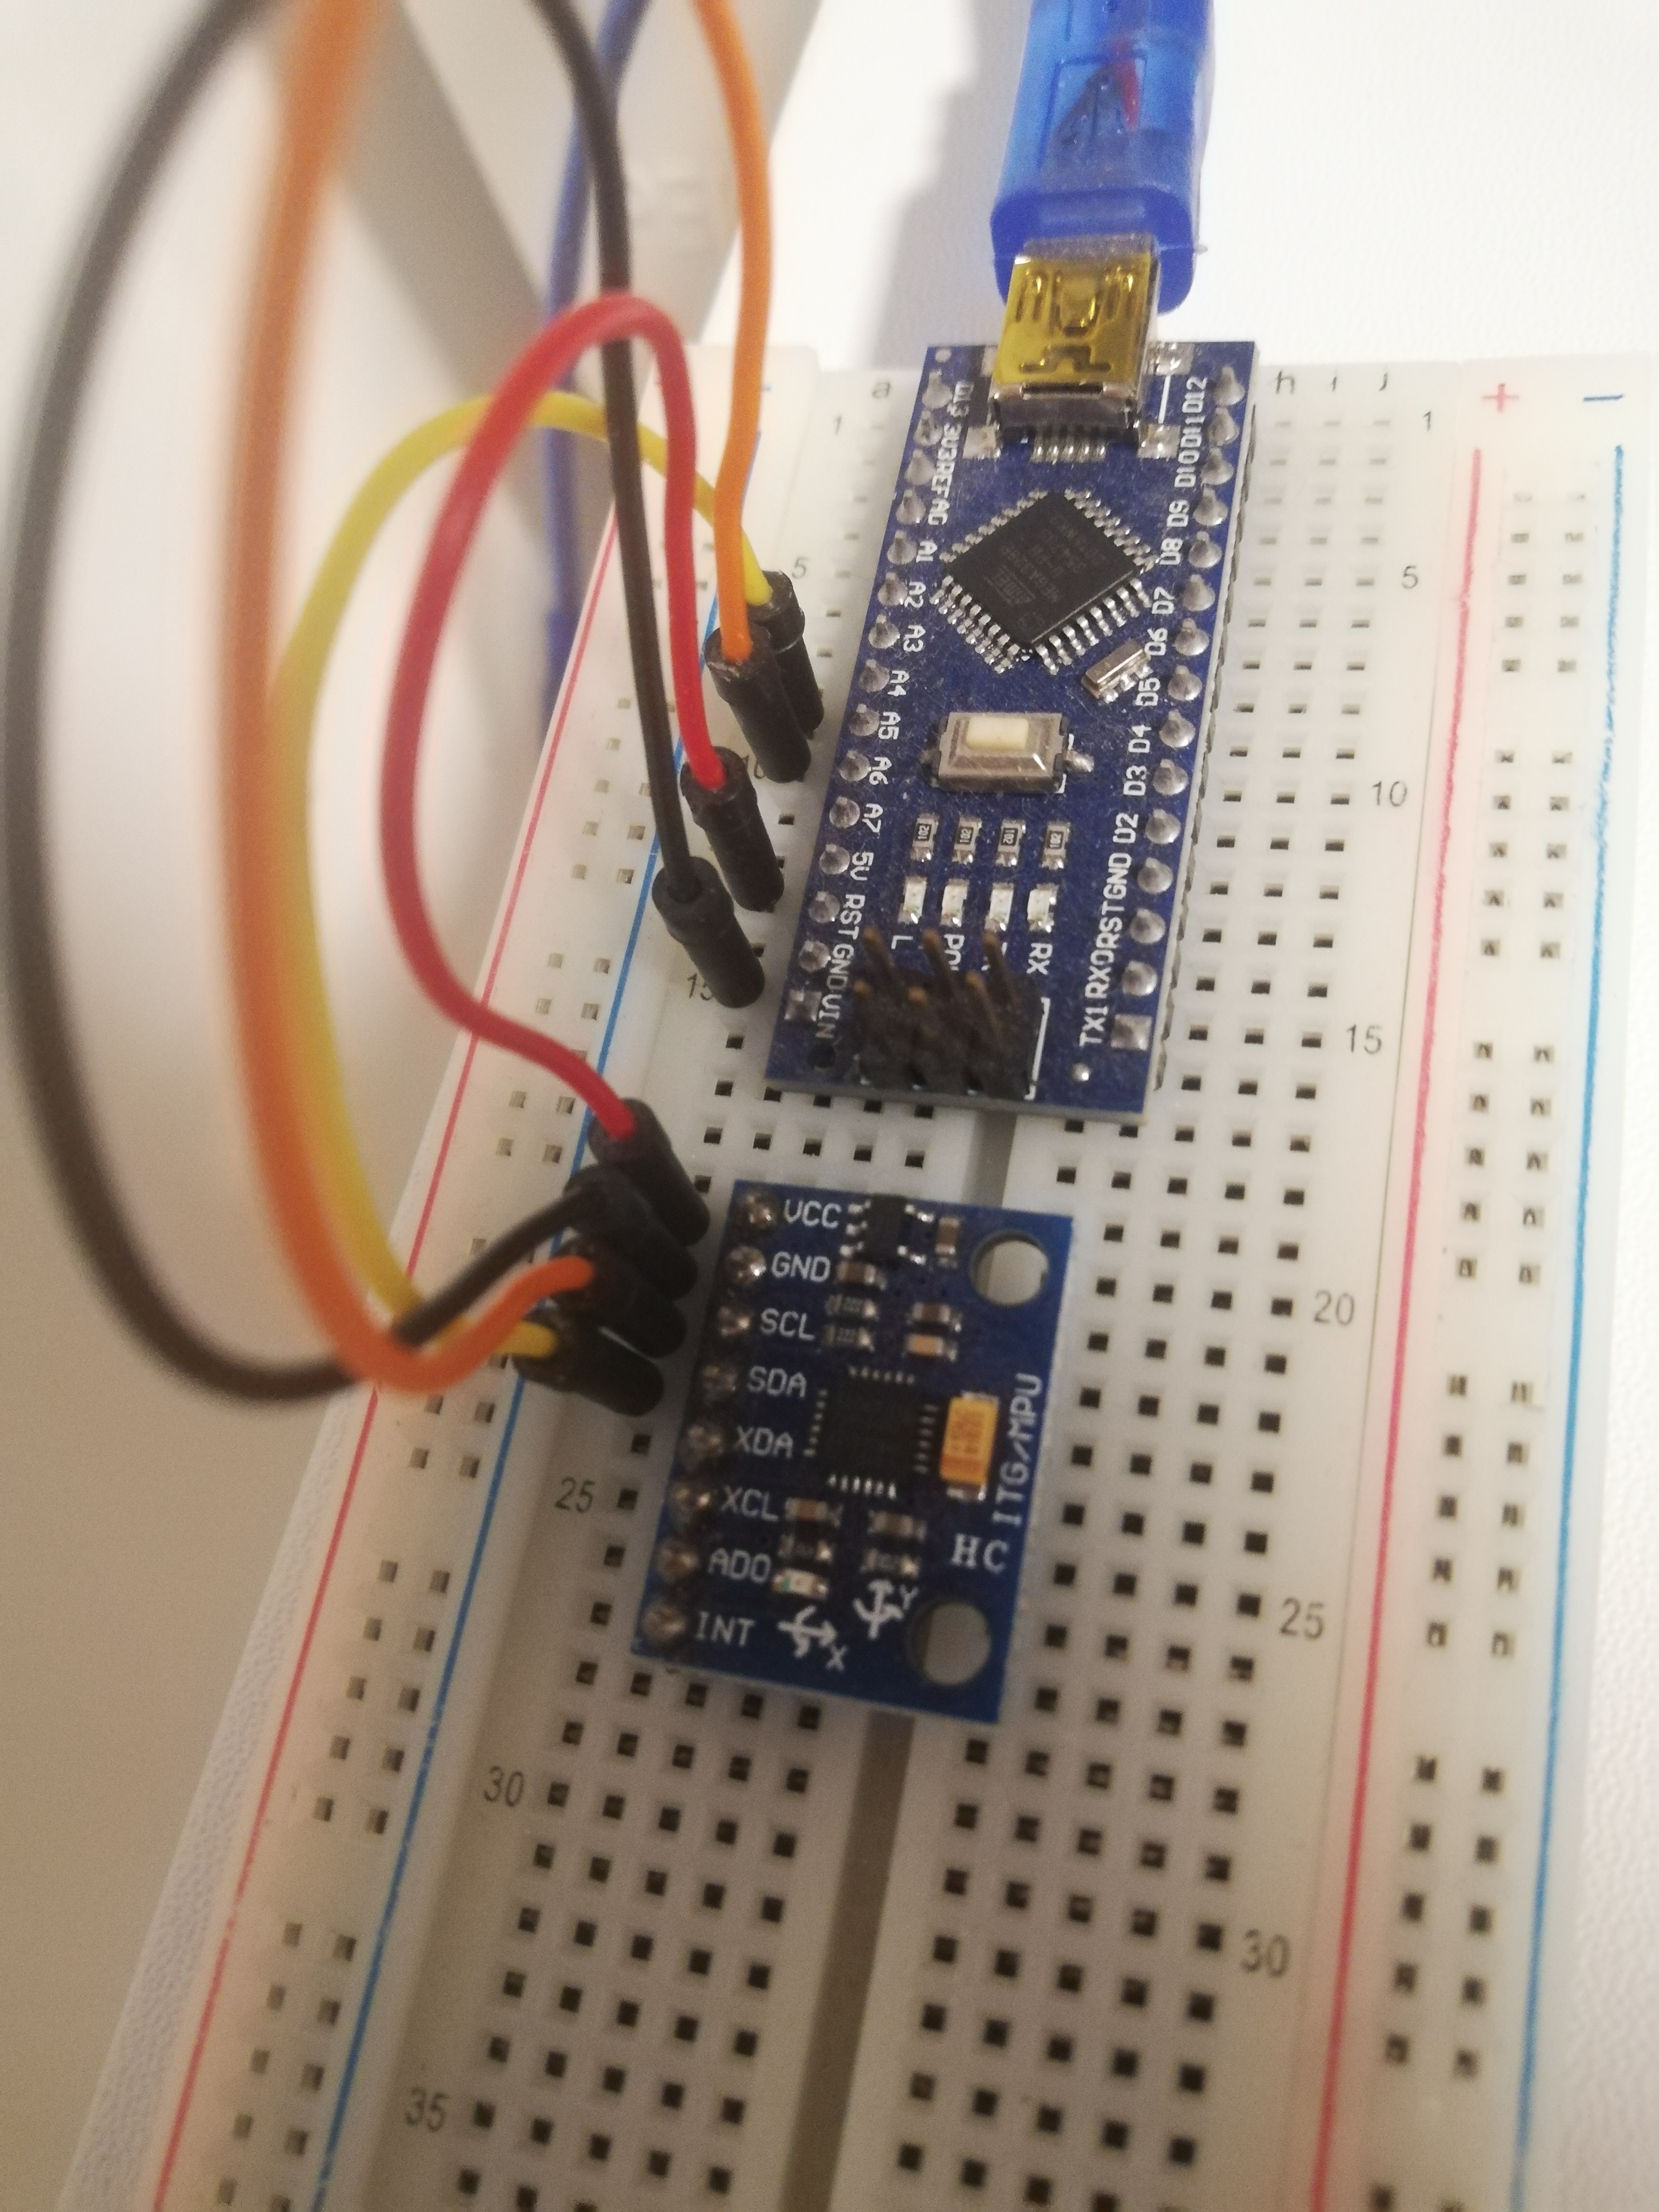
\includegraphics[width=100mm,height=100mm,]{img/arduino}
 \caption{Configura'tie pini}
\end{figure}

Configura'tia se realizeaz'a conform figurii 7.1 'si astfel se alc'atuiesc conexiunile: 


\begin{table}[h]
\centering
\begin{tabular}{|l|l|}\hline
Arduino & MPU-6050 \\ \hline
A5 & SCL \\ \hline
A4 & SDA \\ \hline
VCC & 5V \\ \hline
GND & GND \\ \hline
\end{tabular}
\caption{Conexiune}
\label{tab:my_label}
\end{table}



\section{Resurse software}

Pentru implementarea aplica'tiei a fost folosit programul MATLAB (versiunea 2020b) cu limbajul de programare intrinsec. Toolbox-urile extra folosite sunt \textit{Control System Toolbox} pentru func'tiile \textit{lqr} 'si \textit{place}, \textit{Statistics and Machine Learning Toolbox} pentru vizualizarea histogramelor, pachetul \textit{MATLAB Support Package for Arduino Hardware} pentru conexiunea cu placa \cite{arduino} 'si senzorii \cite{mpu}. Op'tional pot fi folosite resursele din \textit{Sensor Fusion and Tracking Toolbox} pentru vizualizarea 3D a orient'arii 'si \textit{Image Processing Toolbox} pentru facilizarea calcul'arii erorii medie p'atratice. Restul func'tionalit'a'tilor sunt implementa'ri proprii realizate doar cu pachetul individual pus la dispozi'tie 'si concepute cu ajutorul resurselor bibliografice.

\vspace{5px}

Pentru rularea aplica'tiei este necesar ca scripturile de jos s'a fie 'in acela'si director:

\begin{itemize}
    \item QuaternionKalmanFilterModel.m
    \item KalmanFilterModel.m 
    \item VehicleModel2D.m 
    \item ExtendedKalmanFilterModel.m 
    \item ExtendedVehicleModel2D.m 
    \item UnscentedKalmanFilterModel.m 
    \item UnscentedVehicleModel2D.m 
    \item SharkDrawer.m 
    \item SealDrawer.m 
    \item SeagullDrawer.m 
    \item TrackerUI.m 
    \item ObjectTracker.m
\end{itemize}

\textit{ObjectTracker.m} este script-ul principal 'si singurul care trebuie apelat direct de c'atre utilizator. \textit{TrackerUI.m} este func'tia responsabil'a pentru realizarea interfe'tei grafice, 'in timp ce fi'sierele de tip \textit{AnimalDrawer.m} deseneaz'a vectorial 'si integreaz'a cele trei personaje 'in anima'tia principal'a. Clasele filtrelor Kalman 'si ale diferitelor modele de mi'scare sunt cele introduse 'in figura 5.6

\begin{figure}[H]
% \hspace*{-2cm}
\centering
 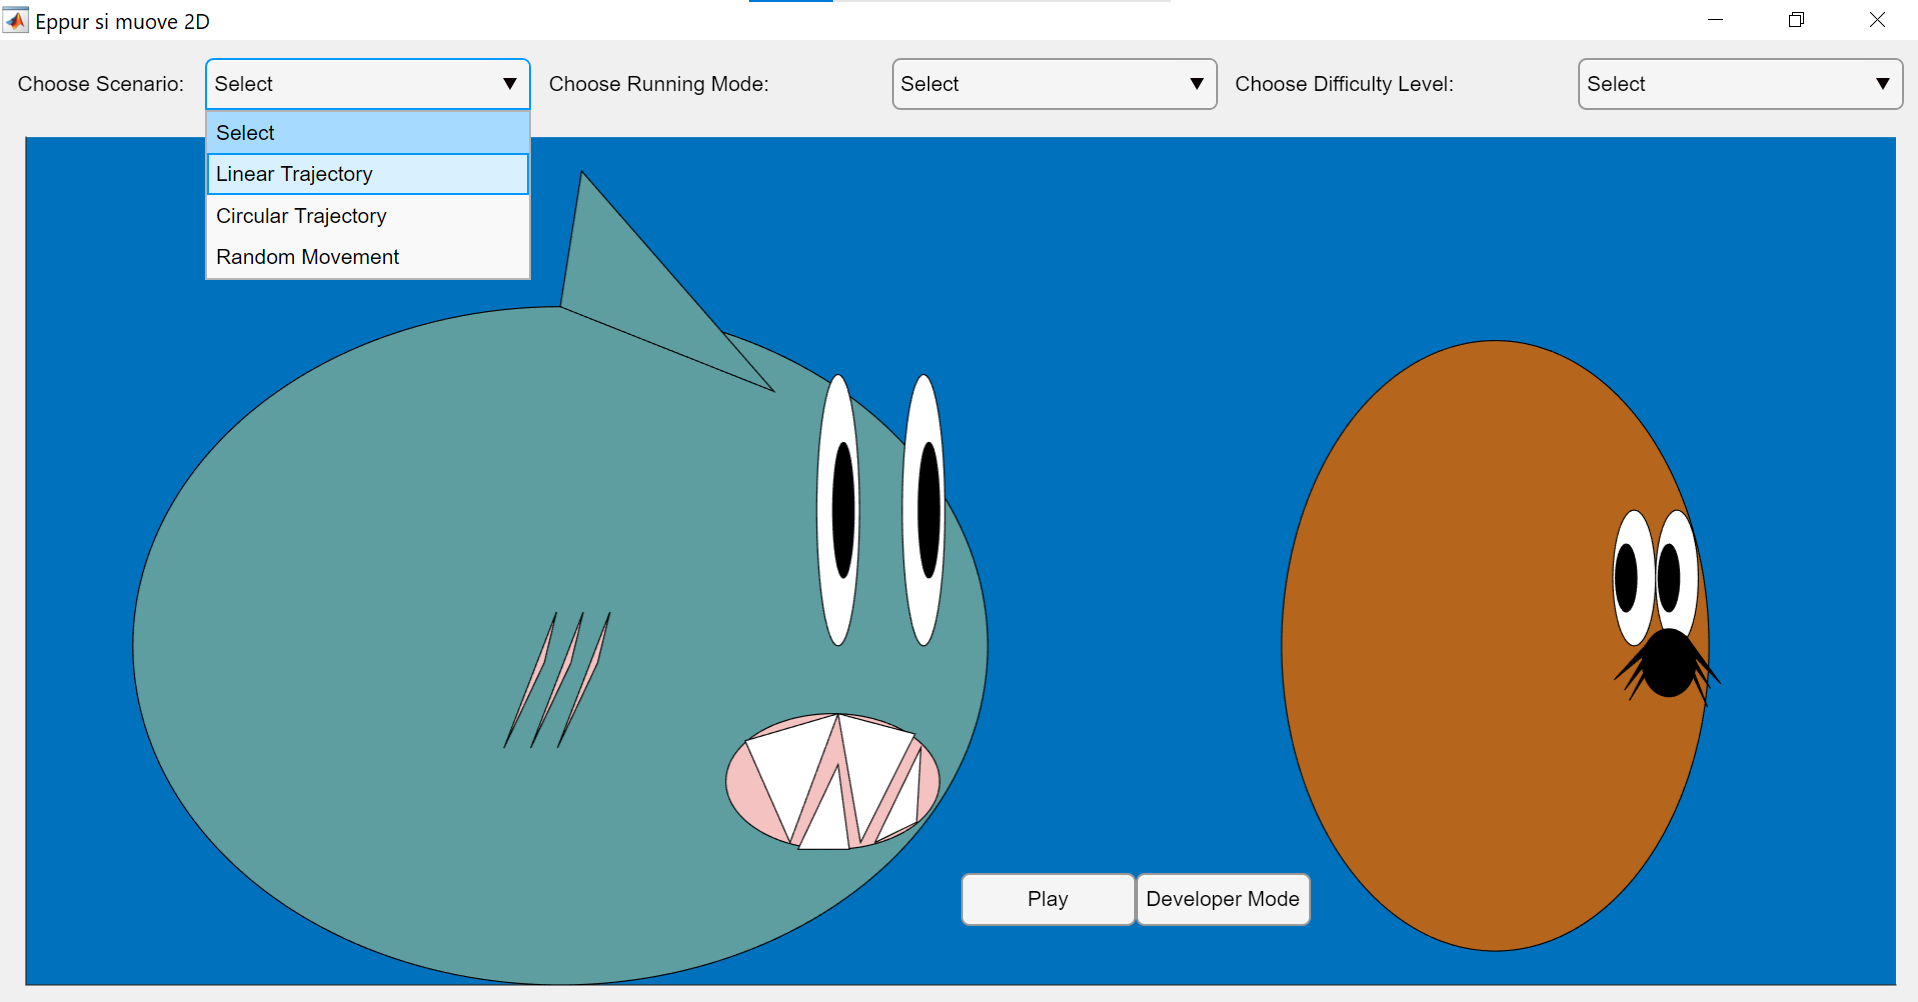
\includegraphics[width=160mm,height=80mm,]{img/scenariujoc}
 \caption{Alegere scenariu}
\end{figure}

\begin{figure}[H]
% \hspace*{-2cm}
\centering
 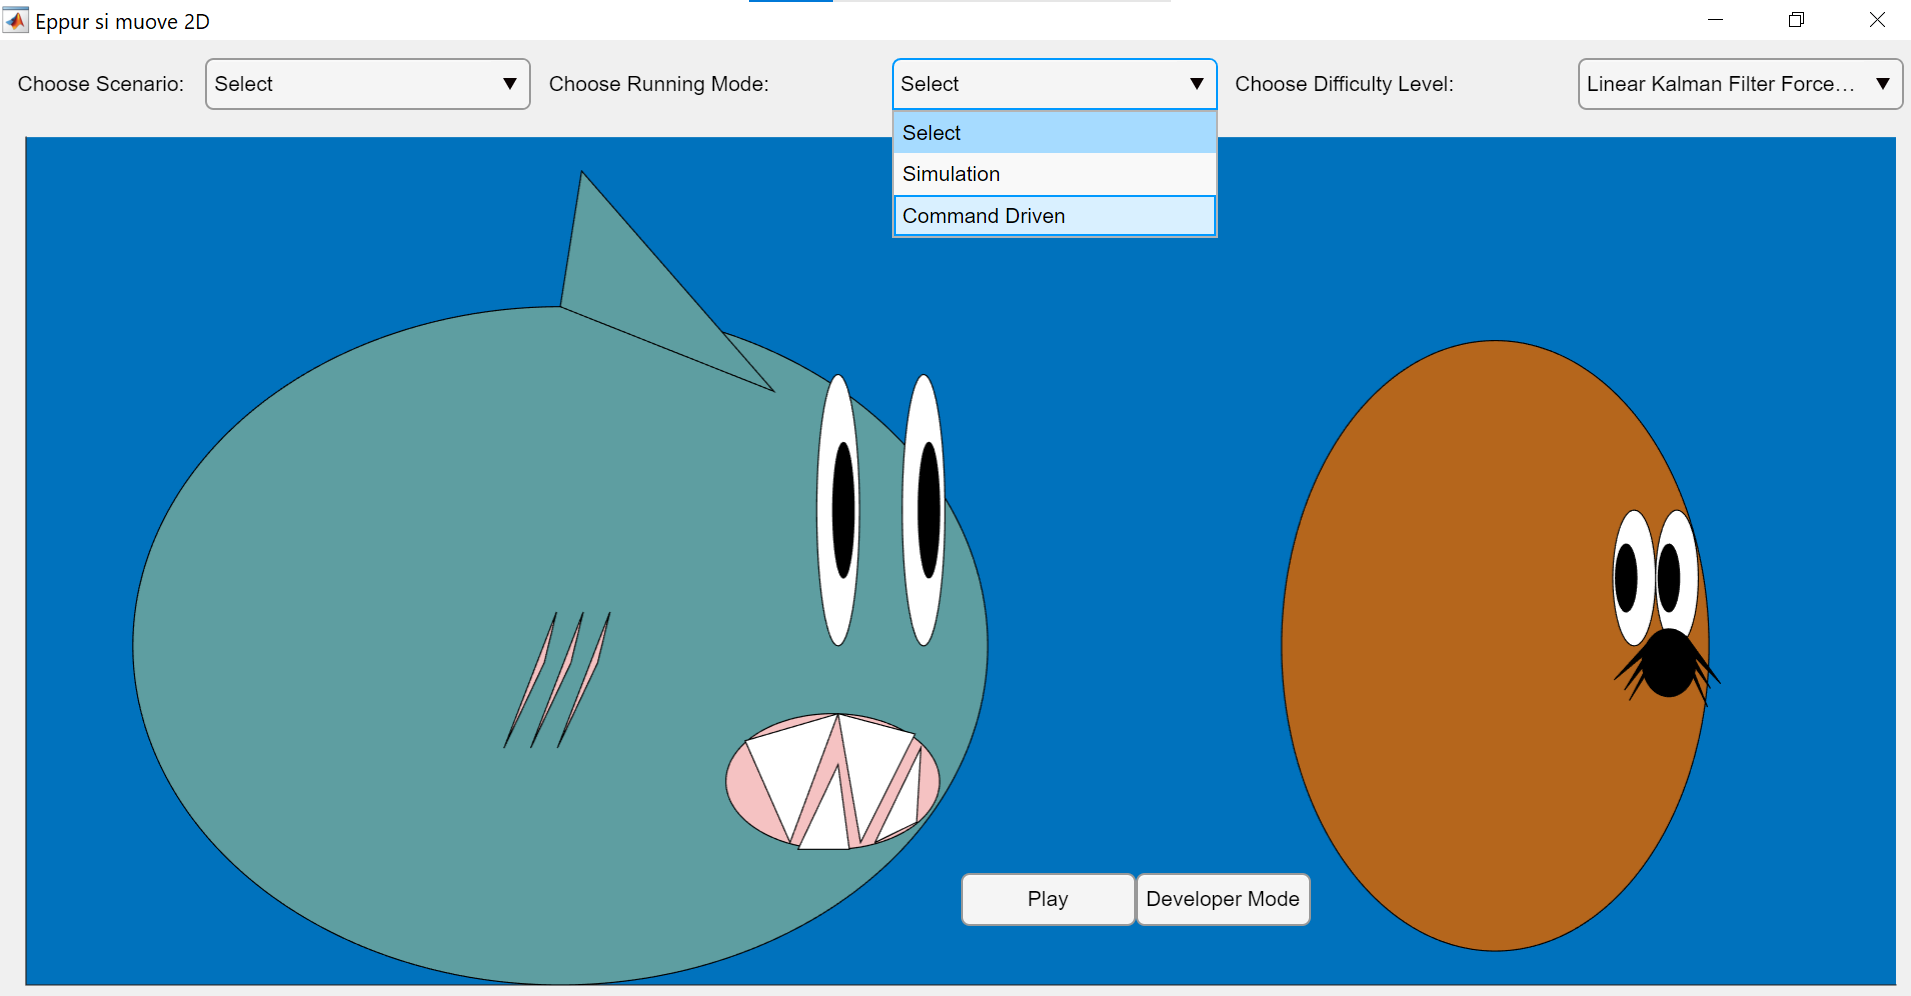
\includegraphics[width=160mm,height=80mm,]{img/runmode}
 \caption{Alegere modalitate de joc}
\end{figure}

\begin{figure}[H]
% \hspace*{-2cm}
\centering
 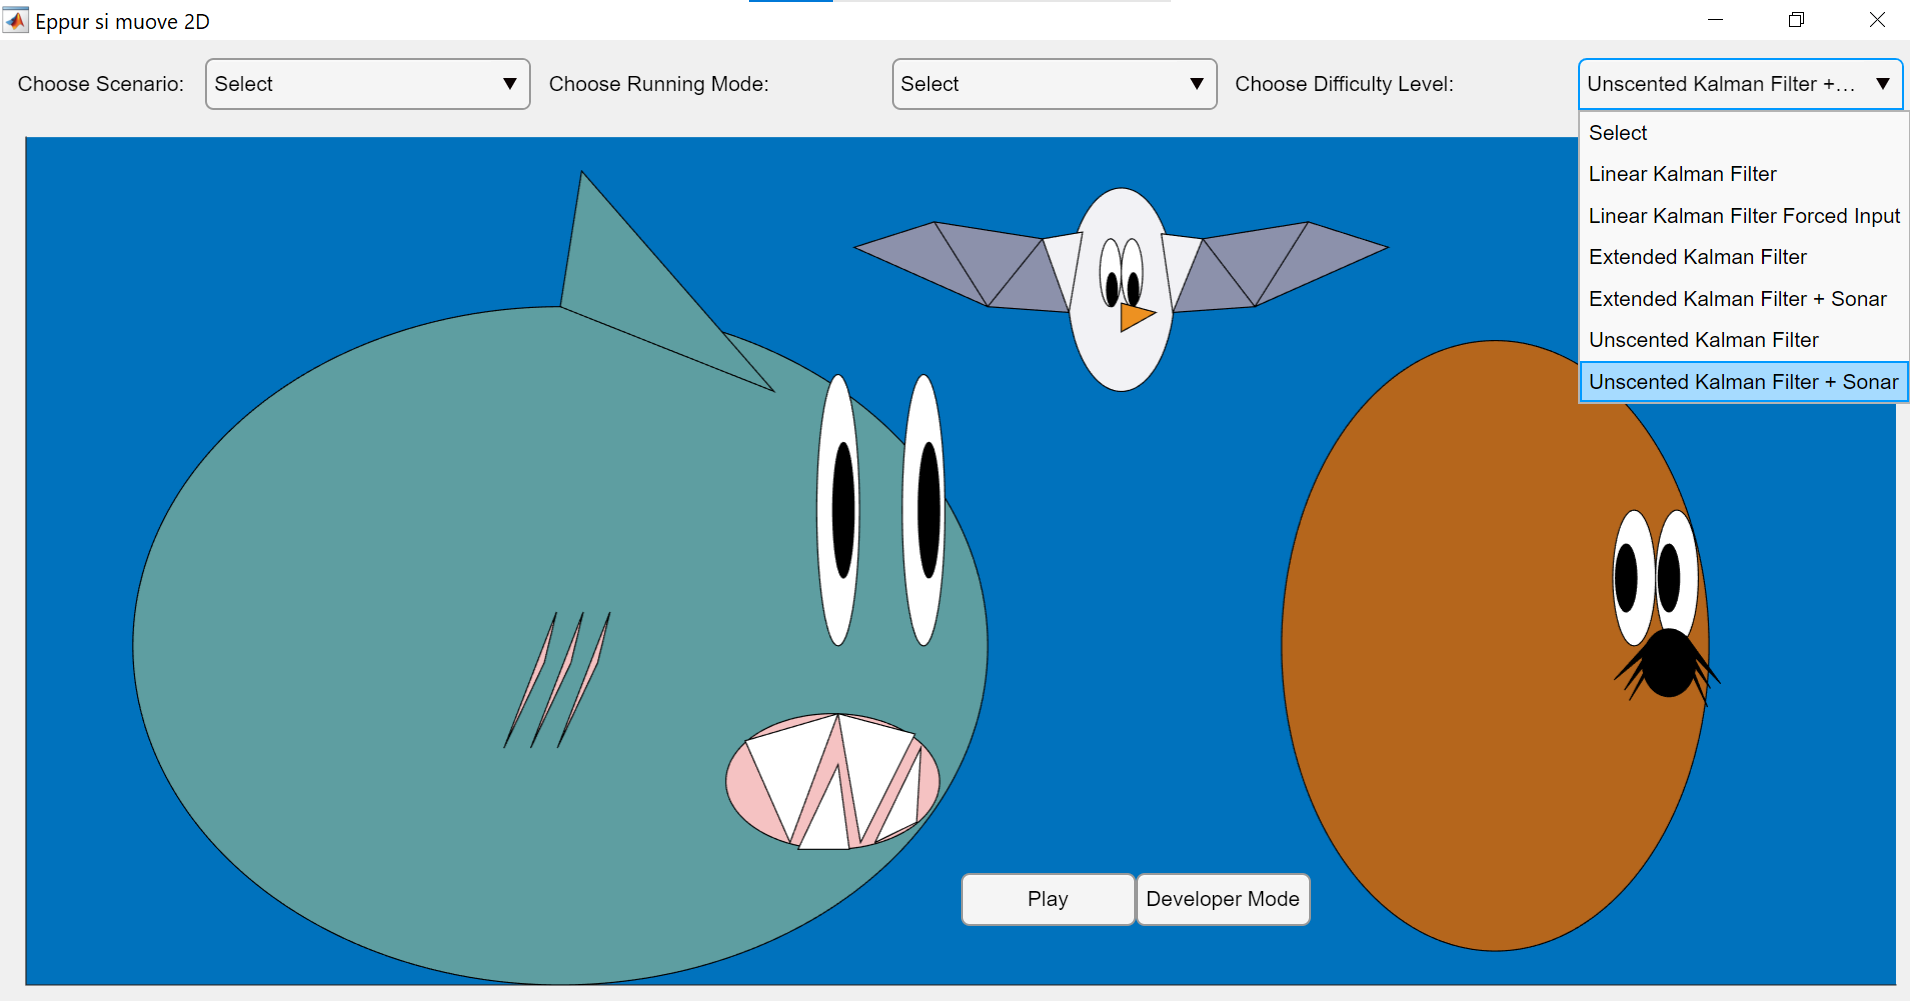
\includegraphics[width=160mm,height=80mm,]{img/dificultate}
 \caption{Alegere estimator}
\end{figure}

\begin{figure}[H]
% \hspace*{-2cm}
\centering
 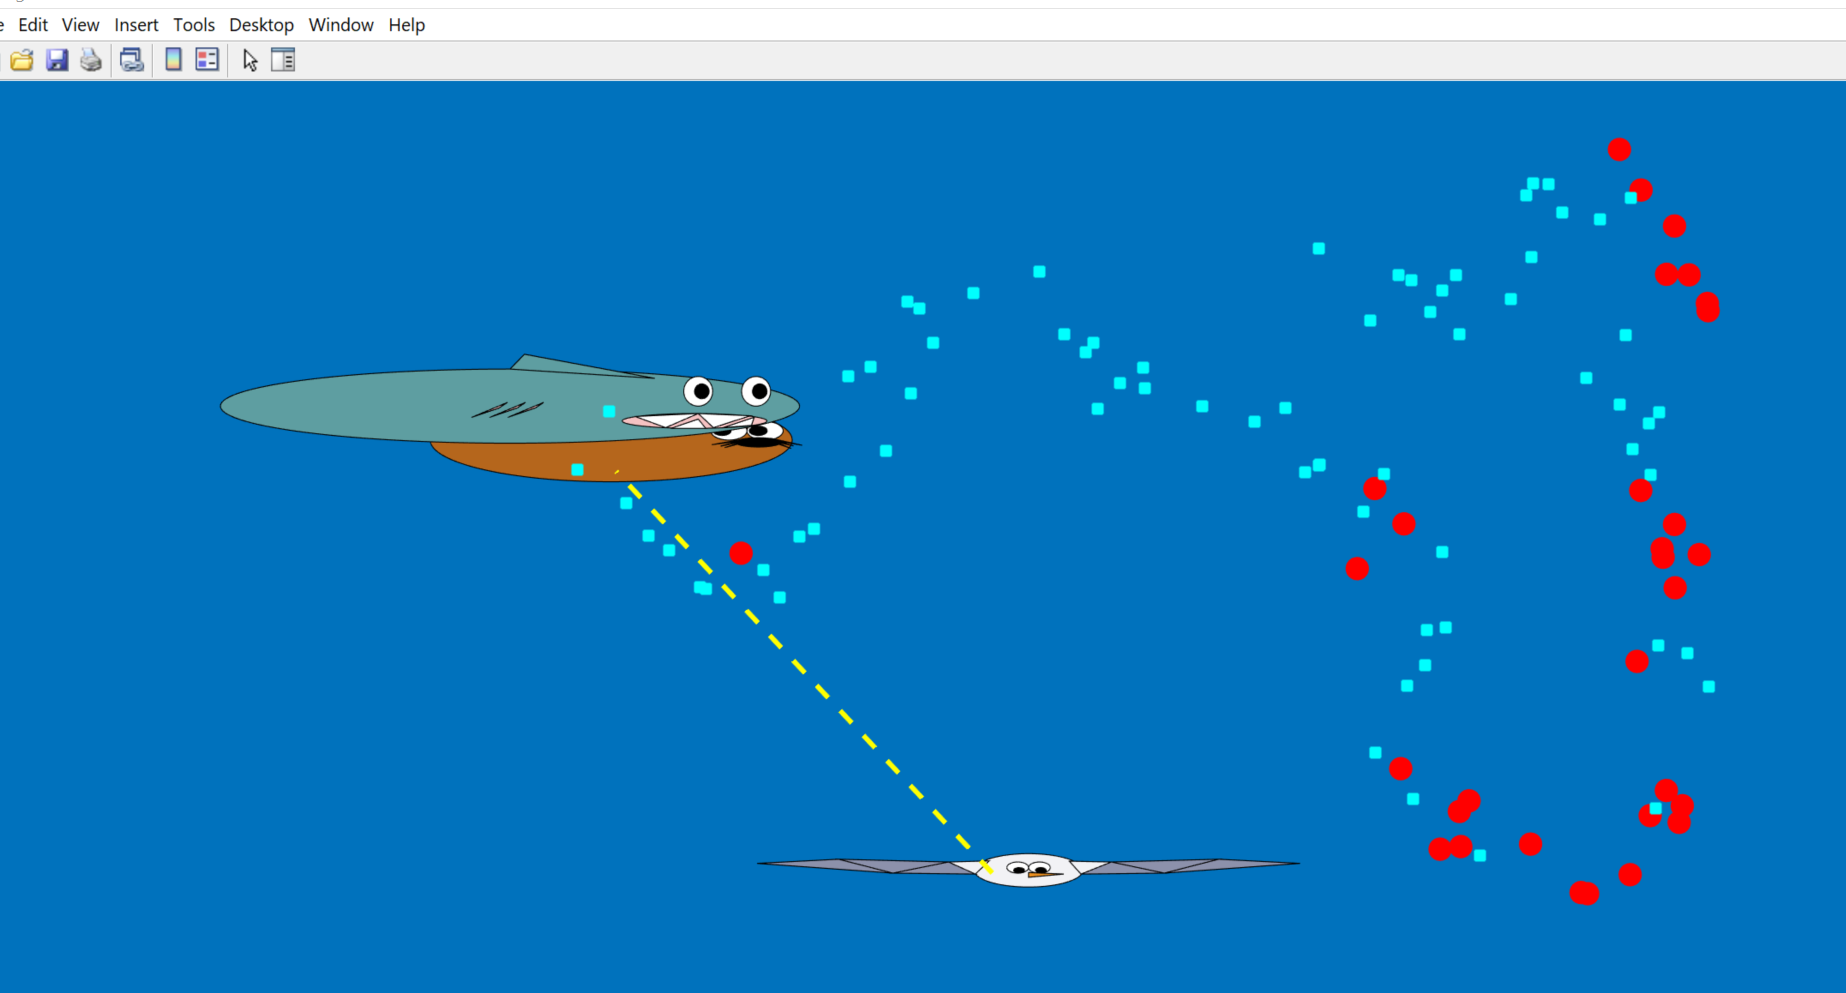
\includegraphics[width=160mm,height=80mm,]{img/race}
 \caption{Desf'a'surare urm'arire}
\end{figure}


Figurile 7.2, 7.3 'si 7.4 prezint'a op'tiunile oferite utilizatorului de interfa'ta grafic'a. Figura 7.5 prezint'a o captur'a a anima'tiei din timpul urm'aririi. 


\chapter{Concluzii}

% Cca. 5\% din total.
% Capitolul ar trebui sa con'tin'a (nu se rezum'a neap'arat la):
% \begin{itemize}
%  \item un rezumat al contribu'tiilor voastre
% \item analiz'a critic'a a rezultatelor ob'tinute
% \item descriere a posibilelor dezvolt'ari 'si 'imbun'at'a'tiri ulterioare
% \end{itemize}

'In 'incheierea acestei lucr'ari, doresc s'a expun o analiz'a critic'a a rezultatelor la care am ajuns p\ia n'a 'in acest punct, presupus'a s'a 'intocmeasc'a o imagine a dezvolt'arilor ulterioare pe care inten'tionez s'a le aduc proiectului prezent. Voi recapitula deci contribu'tiile personale 'si rezultatele ob'tinute 'in scopul sintetiz'arii lucr'arii, dar 'si 'in vederea viitoarelor 'imbun'at'a'tiri.

\section{Contribu'tii}

Am 'incercat prin prezenta lucrare o punere 'in practic'a a diverselor no'tiuni teoretice reg'asite 'in lista bibliografic'a referitoare la algoritmii de estimare 'si fuziune senzorial'a. Am oferit 'in acest sens o implementare personal'a 'in MATLAB pentru modele matematice deja existente 'in literatur'a sau 'in proiecte cu tematic'a, tehnologii sau limbaje diferite.

\vspace{5px}

Am decis s'a dau o not'a accesibil'a conceptelor livre'sti prin scenariul ludic g\ia ndit pentru aplica'tie 'si am descoperit, 'in acela'si timp, c'a un mediu de simulare poate fi folosit 'si pentru dezvoltarea unor aplica'tii diverse prin 'imbinarea no'tiunilor de teorie a sistemelor, controlului 'si estim'arii cu un limbaj de programare de nivel 'inalt, o interfe'ta grafic'a 'si o  vizualizare dinamic'a a performan'telor. 

\vspace{5px}

Am oferit o solu'tie proprie pentru fuzionarea datelor de la un accelerometru 'si un giroscop organiz\ia nd 'si pun\ia nd cap la cap conceptele teoretice 'insu'site din mai multe arii de interes. Aceast'a solu'tie s-a dovedit mai rapid'a dec\ia t preimplementarea oferit'a de mediul de dezvoltare ales, dar nu la fel de exact'a, 'si cu sigurant'a nu la fel de complex'a.

\vspace{5px}

Am reu'sit prin prezenta tez'a s'a adun conceptele teoretice pe care le-am 'inv'a'tat 'in ace'sti ani universitari 'intr-un singur loc, ce pot servi drept suport teoretic implement'arii unor viitoare aplica'tii.

\section{Critic'a}

Dezvoltarea aplica'tiei prezente mi-a permis s'a observ, pe l'ang'a performan'tele algoritmilor folosi'ti, 'si diverse dezavantaje provenite din 'incercarea de a simplifica problematica pentru a ajunge la un rezultat dorit. Simul'arile dinamice 'si interfa't'a animat'a dezvoltat'a mi-au permis s'a observ limit'ari 'intr-un fel 'in care nu a's fi putut s'a o fac doar prin analiz'a teoretic'a. 

\vspace{5px}

Constat astfel cu un ochi critic c'a legile de control liniare folosite sunt limitate pentru scenariul prezent, urm'aritorul nef'ac\ia nd fa't'a de fiecare dat'a schimb'arilor bru'ste de mi'scare. Acest lucru este agravat de faptul c'a regulatoarele simulate dispun de ni'ste performan'te care nici nu ar putea fi implementate 'in practic'a prin natura agresivit'a'tii lor.

\vspace{5px}

Analiz\ia nd partea de estimare, constat cum imii neliniari nu performeaz'a pe at\ia t de bine pe cum ar trebui. De'si 'intr-adev'ar convergen'ta lor nu este garantat'a intrinsec, consider c'a implement'ari mult mai atente ar putea rezolva unele dintre prezentele probleme, cum ar fi convergen'ta covarian'tei odat'a cu starea. Scenariul restr\ia ns bidimensional, de asemenea, devine de la un anumit punct incapabil s'a reproduc'a realitatea. M'asur'atorile de tip GPS 'in realitate nu apar pur 'si simplu pe hart'a, ci sunt recep'tionate prin satelit, deci un estimator al lor de obicei func'tioneaz'a tot prin filtrarea extins'a a unor coordonate transformate 'in polar. Modelul point cloud de reproducere al viziunii sonarului este cu mult simplificat fa't'a de viziunea computerizat'a oferit'a de tehnologii dominante 'in industrie precum senzorii LIDAR. 

\vspace{5px}

Pentru modulul de senzori MPU-6050 nu am oferit o estimare a unghiului de gira'tie, dar trebuie men'tionat c'a func'tia MATLAB \textit{imufilter} ofer'a una, chiar dac'a nu este chiar exact'a. Se pote deduce func'tii trigonometrice pentru unghiul de 'inclina'tie al accelerometrului 'si viteza de rota'tie de pe axa Z a giroscopului poate fi integrat'a numeric 'in timp pentru a oferi o informa'tie despre acesta, dar rezultatul nu era stabil prin lipsa referin'tei. 

\vspace{5px}

Poate chiar mai important, 'si de interes vital pentru o aplica'tie real'a este faptul c'a senzorii nu prezint'a o calibrare riguroas'a, ci doar o eliminare a bias-ului printr-o citire offline anterioar'a. Dup'a cum am men'tionat 'si la 'inceputul lucr'arii, calibrarea senzorilor iner'tiali ar putea constitui o tez'a 'in sine 'si cu siguran't'a reprezint'a ceva ce va trebui analizat minu'tios 'in detaliu. Dac'a senzorii nu sunt calibra'ti corespunz'ator, un algoritm de fuziune nu ar trebui s'a intre 'inc'a 'in discu'tie.

\vspace{5px}

De men'tionat este 'si c'a implementarea proprie a filtrului Kalman bazat pe cuaternioni este liniar'a, ceea ce 'inseamn'a c'a estimatorul, de'si garantat s'a convearg'a, nu va capta 'intreaga dinamic'a a mi'sc'arilor interceptate de senzori, iar acest lucru ar putea fi u'sor depistabil 'intr-o aplca'tie de scal'a mai larg'a. 

\section{Dezvoltare ulterioar'a}

Analiza critic'a a limit'arilor prezentei implement'ari constituie 'si punctul de plecare pentru viitoarele 'imbun'at'a'tiri ale aplica'tiei pe care le consider necesare 'in vederea realiz'arii unui proiect de succes complet. 

\vspace{5px}

Doresc pe aceas'ta cale s'a 'incep dezvoltarea unei aplica'tii cu o grafic'a mai avansat'a tridimensional'a, iar pentru acest lucru inten'tionez s'a folosesc medii de dezvoltare specifice jocurilor video (ex: unreal engine) cu limbaje de programare aferente ($C_{++}$, blueprints) pentru a oferi o perspectiv'a c\ia t mai aproape de realitate a scenariului unei urm'ariri. 

\vspace{5px}

Voi avea 'in vedere pentru imediata dezvoltare legi de control mai avansate, cum ar fi controlul predictiv bazat pe model (MPC) sau controlul prin inteligen't'a artificial'a, iar pentru estimatoare voi 'incerca diferi'ti algoritmi de nivel 'inalt, cum ar fi filtrul de particule, sau algoritmi dedica'ti pentru SLAM.

\vspace{5px}

Doresc de asemenea s'a achizi'tionez 'in viitorul apropiat un modul de senzori MPU-9050 ce extinde capacitatea actualului MPU-6050 folosit prin 'incorporarea unui magnetometru. 'In acest sens, inten'tionez s'a realizez o estimare complet'a 'in spa'tiul tridimensional al orient'arii pentru conceperea unui joystick mai avansat. Acest lucru va impune, bine'inteles, 'si augmentarea algoritmului prezent de fuziune senzorial'a prin ad'ugarea unei noi faze de corec'tie care s'a adreseze noile m'asr'atori.

\vspace{5px}

Tot legat de acest aspect, consider c'a pot explora mai 'in detaliu avantajele folosirii cuaternionilor pentru reprezentarea orient'arii, 'intruc\ia t proiectul de fa't'a nu a intrat 'in profunzimea c\ia 'stigurilor grafice ce pot fi realizate prin tehnici precum SLERP (interpolare sferic'a) pentru netezirea tranzi'tiilor dintre imaginile unei anima'tii, iar acest lucru este c\ia t se poate de realizabil cu fundamentul teoretic pus la dispozi'tie de acest'a lucrare.

\vspace{5px}

Cel mai avansat obiectiv pe care doresc s'a 'il realizez e includerea 'in scenariul urm'aririi unor elemente de viziune computerizat'a, 'inv'a'tare inteligent'a a unui traseu 'in scopul ocolirii unor obstacole sau eficientiz'arii urm'aririi. Doresc astfel s'a realizez un cadru teoretic complet pentru func'tionarea vehiculelor autonome din actuala industrie emergent'a.

%\addcontentsline {toc}{chapter}{Bibliography} 
\bibliographystyle{IEEEtran} 
\bibliography{thesis}%same file name as for .bib

\appendix
\chapter{Clasa UKF - Implementare 'in MATLAB}


\lstinputlisting[language=Matlab, xleftmargin=-25mm,basicstyle=\tiny]{UnscentedKalmanFilterModel.m}



\chapter{Calibrarea giroscopului prin 'inv'a'tare automat'a}

'Intruc\ia t nu am epuizat subiectul calibr'arii senzorilor folosi'ti 'in lucrarea propriu-zis'a, am decis s'a dedic aceast'a anex'a pentru redijarea complexului fenomen, deoarece consider c'a 'intelegerea lui nu poate fi privit'a unilateral fat'a de algoritmii de fuziune senzorial'a.

\vspace{5px}

M'asur'atorile senzorilor giroscopici sunt afectate de temperatur'a \footnote{Nez, Alexis & Fradet, Laetitia \& Laguillaumie, Pierre & Monnet, Tony & Lacouture, Patrick. (2018). Simple and efficient thermal calibration for MEMS gyroscopes. Medical Engineering & Physics. 55.10.1016/j.medengphy.2018.03.002.}, iar acest lucru provoc'a fenomenul de \textit{drift} men'tionat la 'inceputul lucr'arii. De obicei, dac'a temperatura senzorului sau a pl'acii de care este ata'sat cre'ste constant, atunci 'si \textit{drift-ul} va cres'te constant, 'si poate fi aproximat simplu printr-o regresie liniar'a (4.90) - (4.102), sau integrat 'in vectorul de stare al filtrului Kalman pentru a fi estimat odat'a cu orientarea. 

\vspace{5px}

Doresc s'a prezint 'ins'a 'in aceast'a parte a lucr'arii un caz neliniar de cres'tere a temperaturii ce produce ridica'ri 'si sc'aderi 'in media m'asur'atorilor pentru o perioad'a mai lung'a de timp. Am realizat astfel un experiment prin pornirea 'si oprirea unui ventilator extern pentru laptopul la care erau conectate placa de dezvoltare 'si modulul de senzori 'si am 'inregistrat datele citite de la senzori pentru 30000 de itera'tii (aproximativ 60 de minute).

\vspace{5px}

Se poate constata cum m'asur'atorile giroscopului de pe axa X au fost deviate 'in figura B.1. M'asur'atorile accelerometrului 'in schimb nu au fost deloc afectate de schimbarea de temperatur'a pentru nicuna dintre cele trei axe. Pentru c'a zgomotul prezent era mult prea mare, am aplicat setului de date un filtru de mediere pentru o fereastr'a de $\pm 10$ valori, 'si am testat experimentul doar pentru axa ruliu:

\begin{gather}
    f(X) = \frac{\sum_{i=t-10}^{t+10} X_i}{2 \times 10 + 1}
\end{gather}

\begin{figure}[h]
  \hspace*{-4cm}
  \includesvg{img/processing.svg}
  \caption{Corec'tie m'asur'atori}
\end{figure}

Am proiectat apoi pentru datele filtrate o re'tea neuronal'a cu ajutorului submodulului \textit{nn} din PyTorch folosind fun'ctii de activare liniare de baz'a 'si func'tia ReLU \footnote{https://pytorch.org/docs/stable/generated/torch.nn.ReLU.html} (Rectified Linear Unit) pentru a putea descoperi neliniarit'a'tiile 'in propagarea re'telei 'inapoi. 

\vspace{5px}

Pentru ca re'teaua s'a fie capabil'a s'a mimeze toate iregularit'a'tile prezente a fost nevoie de introducere unui num'ar mare de neuroni pentru straturile ascunse, 'si am g'asit empiric c'a un num'ar potrivit este de 25 de neuroni ca l'at'ime pentru o ad\ia ncime de dou'a straturi suplimentare. Am conceput astfel re'teaua neuronal'a conform figurii B.2 \footnote{https://alexlenail.me/NN-SVG/index.html}:

\begin{figure}[h]
%   \hspace*{-3.5cm}
\centering
  \includesvg[width=150mm,scale=1]{img/nn.svg}
  \caption{Re'tea neuronal'a}
\end{figure}

Unde penultimul strat ascuns format dintr-un singur neuron are doar rolul s'a mai treac'a o dat'a rezultatul prin activarea neliniar'a 'inainte de procesarea final'a. Astfel, pentru un neuron de la intrare (pentru un element din vectorul de date) se repet'a propagarea p\ia n'a la ob'tinerea rezultatului (neuronul de ie'sire, valoarea punctului transformat'a).

\vspace{5px}

Deoarece corela'tia dintre doi vectori poate fi ob'tinut'a prin calcularea erorii dintre fiecare element asociat unei itera'tii specifice, am ales s'a folosesc func'tie \textit{MSELoss} \footnote{https://pytorch.org/docs/stable/generated/torch.nn.MSELoss.html} ce returneaz'a erorea medie p'atratic'a dintre vectorul ini'tial 'si rezultatul procesat. Astfel, am proiectat algoritmul 'in felul urm'ator: 


\begin{algorithm}
\caption{Propagare re'tea neuronal'a (Pseudo-Python)}
\begin{algorithmic} 
\REQUIRE  x = vector itera'tii, y = vector valori giro
\ENSURE $y,x = float \wedge y,x = torch.tensor$
\ENSURE MSELoss()
\ENSURE $nn(Linear(1,25),ReLU(),Linear(25,25),ReLU(),Linear(25,1),ReLU(),Linear(1,1)$
\ENSURE Optimizator = Stochastic Gradient Descent 
\STATE $ pas \leftarrow 0.05$
\STATE $epoci \leftarrow 700$
\FOR{(epoc'a din epoci)}
\STATE $\hat y \leftarrow nn(x)$
\STATE MSELoss($\hat y, y$)
\STATE MSELoss.backward()
\STATE Optimizator.gradient\_zero()
\STATE Optimizator.propagare(pas)
\ENDFOR
\end{algorithmic}
\end{algorithm}

Pentru care \textit{pas-ul} reprezint'a valoarea cu care 'inainteaz'a func'tia de gradient (optimizatorul) pentru minimizarea erorii p'atratice, iar func'tiile de tip \textit{backward} \footnote{https://pytorch.org/docs/stable/generated/torch.Tensor.backward.html}, \textit{gradient\_zero} \footnote{https://pytorch.org/docs/stable/generated/torch.optim.Optimizer.zero_grad.html} 'si \textit{propagare} \footnote{https://pytorch.org/docs/stable/generated/torch.optim.Optimizer.step.html} reprezint'a faza de evaluare invers'a a re'telei 'in scopul calcul'arii ponderilor prin func'tiile de activare neliniare ReLU. Aceste ponderi rezultate sunt cele care decif magnitudinea r'aspunsului final pentru fiecare epoc'a 'si astfel se ob'tine un vector ca 'in figurra B.3, 'in al c'arei prim grafic se observ'a c'a valorile tensorului ini'tial au fost extrapolate corect de re'tea cu o valoare de corela'tie de 89\% \footnote{https://numpy.org/doc/stable/reference/generated/numpy.corrcoef.html} 'intre adev'ar 'si predic'tie.

\vspace{5px}

A doua parte a figurii prezint'a minimizarea func'tiei de cost (eroarea medie p'atratic'a atinge valoarea minimi'a posibil'a) 'si se constat'a cum un num'ar mai redus de epoci ar putea fi suficient pentru antrenarea re'telei, 'intruc\ia t sc'aderea nu mai este drastic'a dup'a primele 200 de epoci. 
\vspace{5px}

Rezultatul final ob'tinut prin sc'aderea fomei recuperate din datele reale se reg'ase'ste 'in al doilea grafic din figura B.1 'si se poate constata c'a astfel s-a redus 'si bias-ul static, dar 'si evolu'tia driftului.

\begin{figure}[h]
  \hspace*{-3.5cm}
  \includesvg{img/MLcalib.svg}
  \caption{Predic'tie re'tea neuronal'a}
\end{figure}

Desigur, pentru un astfel de exemplu trebuie men'tionat c'a o aproximare polinomial'a ar fi func'tionat probabil mai bine 'si mai eficient, f'ar'a a avea nevoie de timp de antrenare, 'si f'ar'a a putea oferi rezultate gre'site. Un model matematic bazat pe un proces va fi mereu de preferat 'in locul unuia bazat pe 'inv'a'tare, dac'a procesul este determinist.

\vspace{5px}

Cu toate acestea, consider c'a acest tip de metode de calibrare deschide noi perspective pentru senzorii iner'tiali, 'intruc\ia t extrapolarea inteligent'a a unui semnal se poate adapta 'si 'in cazul 'in care acesta 'isi schimb'a comportamentul 'intr-un mod stocastic.

\vspace{5px}

Deoarece acest comportament al m'asur'atorilor senzorului a fost ob'tinut 'intr-un timp de lung'a durat'a comparativ cu minutele de obicei alocate unui joc, 'si pentru c'a ob'tinerea drift-ului a necesitat interven'tie exterioar'a prin modificarea activ'a a temperaturii, acest model nu a fost inclus 'in aplica'tia final'a, dar doresc, prin 'incheierea acestei anexe, s'a pun bazele unei posibile dezvolt'ari ulterioare a unui algoritm de estimare a orient'arii bazat pe inteligen't'a artificial'a.



\chapter{Lucr'ari publicate}

A. Moraru, "Quaternion Based Kalman Filter for Open Loop Attitude Estimation", AQTR Student Forum, p. 29, Aprilie 2022

\end{document}
